\lohead{Dominik Pichler}
\chapter{Mechanik}
\section{Einleitung}

Aufgabe dieses Teiles war die Umsetzung des mechanischen Aspekts der Arbeit. Des Weiteren galt es den effizientesten Weg des Fütterungsprozesses zu ermitteln.

\section{Aufgabenstellung und Zielsetzung}

Ziel ist es, eine Katzenfütterungsanlage zu entwickeln. Ausgangslage sind Katzenfutterbeutel aus Aluminium-Kunststoff-Folie. Die Fütterung mit Dosen wird hier betrachtet. Das Futter soll zeitlich gesteuert in den Behälter gefüllt werden und so der Katze zugänglich gemacht werden und die leeren Beutel geruchsisoliert entsorgt werden. Die Anlage soll zum Beispiel während Kurzurlauben oder zum normalen Füttern der Katze oder des Hundes verwendet werden. Nach Aktivieren der Anlage wird in davor gewählten definierten Zeitpunkten die Katze gefüttert. 


\section{Problematik}

Jede Variante in den unten beschrieben Maschinen weißen Schwächen bzw. Probleme auf. Diese werden in den folgenden Punkten erläutert.

\subsection{Problematik des automatisierten Aufschneidens}

Das Problem des automatischen Schneiden ist, dass das Material der Verpackung sehr zäh ist und eine hohe Zugfestigkeit hat. Darum ist ein hoher Anpressdruck zwischen den Klingen erforderlich. Zudem darf die Klinge, auch wenn sie lang ist, nicht verbiegen. Damit die Aluminium-Kunststoff-Folie nicht zwischen den Klinge gelangt und diese auseinander presst. Das hat Zufolge, dass das die Packung zerknittert und schwerer zu schneiden ist. 

\subsection{Problematik der Dichtheit bei Klemmen}

Bei der zweiten Variante wird erwartet das der Besitzer die Packung aufschneidet und eine Klemme befestigt. Diese muss mindestens fünf Tage lang dicht halten damit die Maschine nicht verschmutzt und die Katze etwas zu fressen hat. Wenn die Katzenfutterpackung nicht dicht ist gelangt Luft hinein und das gesamte Futter trocknet ein, somit lässt sich das ganze Futter noch schwerer aus der Verpackung pressen. Des weiteren kann das Futter verderben wenn Luft eindringt. Auch bei geringer Veränderung des Futters kann es sein, dass die Katze, das Futter nicht frisst.

\subsection{Problematik bei Entleerung der Verpackung}

Beim Entleeren der Verpackung bei geleeartiger Füllung treten einige Probleme auf die sich meist nur mit dem Pressen der Verpackung lösen lassen. Das Futter kann erstens in der Verpackung auf der Folie haften und somit durch die Schwerkraft nicht vollständig entleert werden. Zweitens die Luft muss von der Öffnung bis zur geschlossenen Seite gelangt, damit der Luftdruck nicht das Entleeren verhindert(ähnlich wie beim Entleeren einer volle Ketchupflasche). 

\subsection{Problematik vom Geruch}

Bei automatischen Füttern eine Katze ist der Geruch ein großes Problem, da Katzenfutter schon am ersten Tag einen strengen Geruch hat und der sich über die Tage steigert. Die einzige Maßnahme die getroffen werden kann, ist die ganze Maschine Luftdicht zu gestalten (die einzige Ausnahme wäre, wenn es den Benutzer nicht stört und ihm das wichtigste ist, dass dieser erleichtert ist wenn seine Katze gefüttert ist). 

\subsection{Problematik von der Reinigung nach dem Urlaub}

Durch das Pressen der Packungen kann das Gelee an der Walze bleiben und diese verschmutzen. Die gedachte Lösung ist, dass das Gehäuse aufklappbar ist. Das bedeutet dass der Benutzer mit viel Freiraum in die Maschine greifen kann und  somit die beiden Walzen reinigen kann. Die Futterschüsseln lasse sich durch die Konstruktion der unten beschriebene Variante (Drehplatte) leicht entfernen. Die Futterplatte kann bei Verschmutzung durch ihre wasserfeste Beschichtung gereinigt werden.

\subsection{Problematik beim Einfrieren des Futters}

Wenn man das Futter einfriert braucht man durchgehend Energie zum Betreiben der Gefriertruhe. Außerdem wird viel mehr Platz benötigt und der Kompressor macht Lärm. Des weiteren ist das Dichthalten der Truhe ein großes Problem, da der Greifer an einen bestimmten Punkt in die Maschine eindringen muss, um die gefrorene Portion in den Behälter zu befördern. Wenn die Truhe nicht dicht hält, schmilzt der Inhalt und das Futter verdirbt.

\section{Konzepte} 

In den folgenden Punkten werden die verschiedenen Varianten vorgestellt. Des weiteren werden durch Schemenskizzen die einzelnen Varianten verdeutlicht um so einen Eindruck der zu realisierenden Maschine zu erhalten.

\subsection{Variante 1: Automatisiertes Aufschneiden} 

Diese Variante wurde durchdacht um einen Eindruck zu erhalten, wie das automatische Schneiden funktionieren könnte. Welche Probleme es aufwirft und welche Vorteile es gibt soll analysiert werden.

\subsubsection{Übersicht der Prozessschritte}

In den folgenden aufgelisteten Schritten werden die einzelnen Punkte erläutert und anhand von Fotos der mit Lego gebauten Variante in verschiedenen Ansichten gezeigt.

\begin{itemize}
\item[1] Füllen des Futtermagazins
\item[2] Führen zur Schneidplatte
\item[3] Schnitt
\item[4] Pressen
\item[5] Entsorgen
\item[6] Füttern
\item[7] Abtransport der Tasse vor dem nächsten Füttern.
\end{itemize}


\newpage
\subsubsection{Füllen des Futtermagazins}


\begin{wrapfigure}{r}{0.5\textwidth}
\vspace{-30pt}
  \begin{center}
    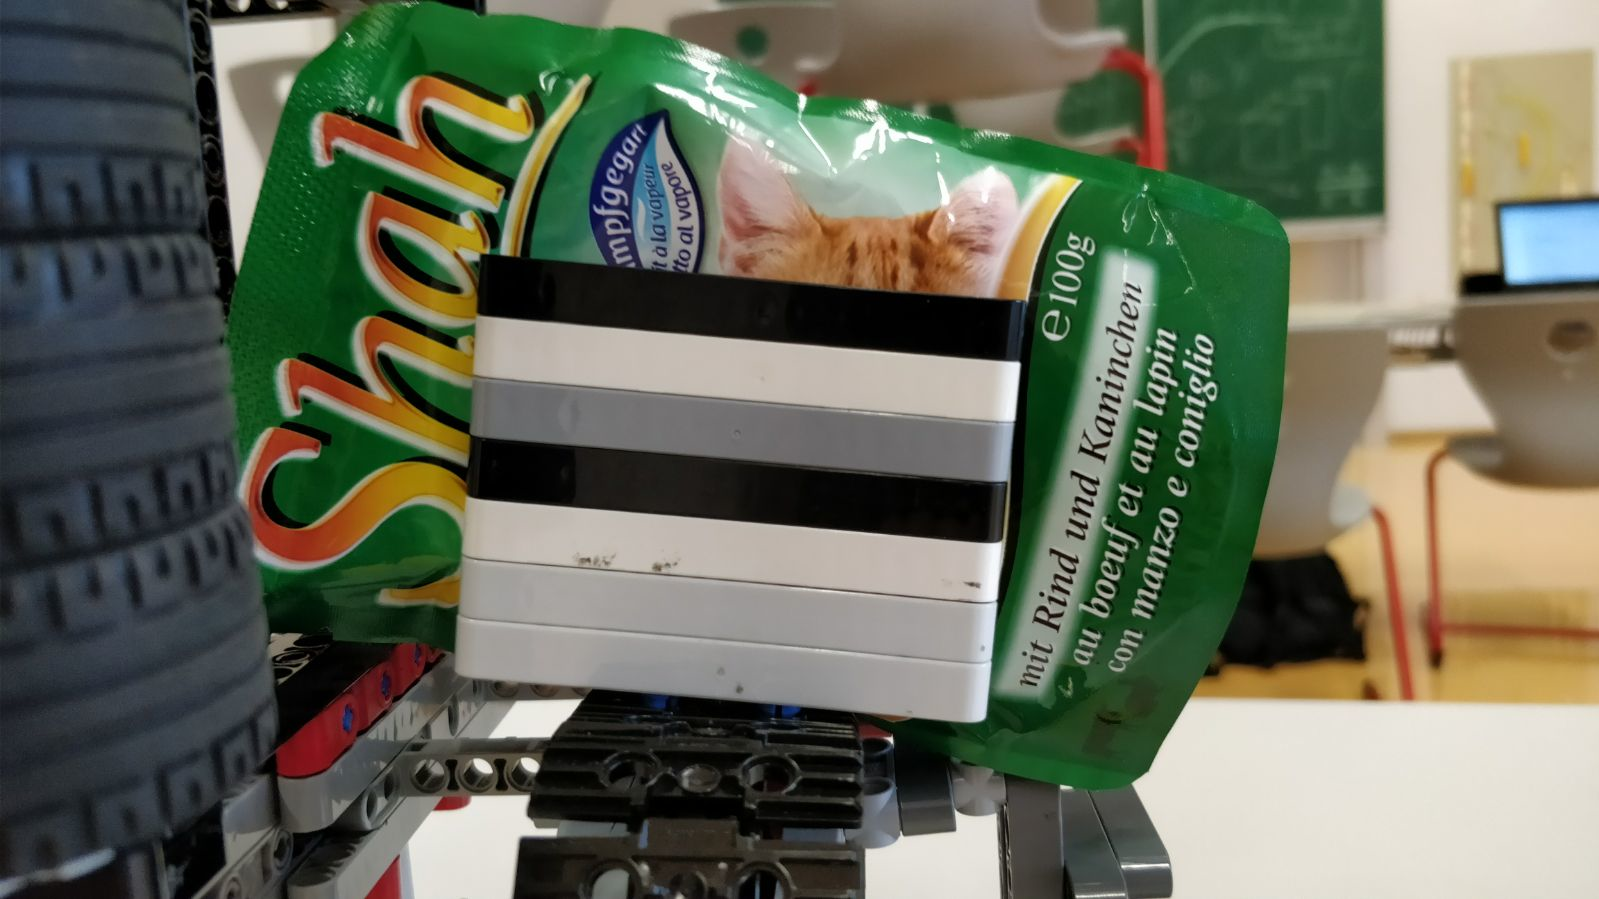
\includegraphics[width=0.50\textwidth]{Bilder/Ablauf_1_png/Magazin_Vorne}
  \end{center}
  \caption{Magazin Modellaufbau von Vorne}
  \label{Magazin Vorne}
  \vspace{-10pt}
\end{wrapfigure}

In den folgenden Bildern wird das Magazin anhand eines Aufbaues aus Lego in verschiedenen Blickwinkeln gezeigt. Hier muss man beachten ,dass die vom Futterhersteller für die Öffnung vorgesehene Seite in Richtung des Schneidewerks zeigt (die schmale Seite mit der Einkerbung). Siehe Abbildung: \ref{Magazin Vorne}.
Das ganze Förderband besteht grundsätzlich aus der Halterung die das Magazin in einer bestimmten Höhe hält, damit die einzelnen Trennwände nicht mit dem Boden kollidieren. Der Oberteil des Bandes schließt eben mit der Schneideplattenhöhe ab um ein leichtes Gleiten der Packung durch den Greifer zu ermöglichen, ohne dass es Höhenunterschiede überwinden muss. Des weiteren wird über zwei Räder ein Band gespannt an denen die Trennwände in Abstand der Dicke der Packung festgemacht werden. Das Band wird mithilfe eines Motors in Bewegung gebracht und kann somit von Abteil zu Abteil bewegt werden , um immer nach dem Füttern eine neue Packung bereit zu stellen. Auf diesem Band kann je nach Länge eine gewisse Anzahl an Futterpackung abgelegt werden, natürlich nur auf der Oberseite, da die Packungen ansonsten aus den Abteilungen fallen würden. Die Trennwände sind zum Startzeitpunkt alle auf der Oberseite. In diesem Magazin hätten 7 Packungen platz.\\

In Abbildung: \ref{Magazin Seitlich} wird das Magazin von der Seite gezeigt. \\
In Abbildung: \ref{Magazin Oben} wird das Magazin von Oben gezeigt. 

\begin{figure}[H]
   \begin{minipage}[hbt]{0.5\textwidth} % [b] => Ausrichtung an \caption
      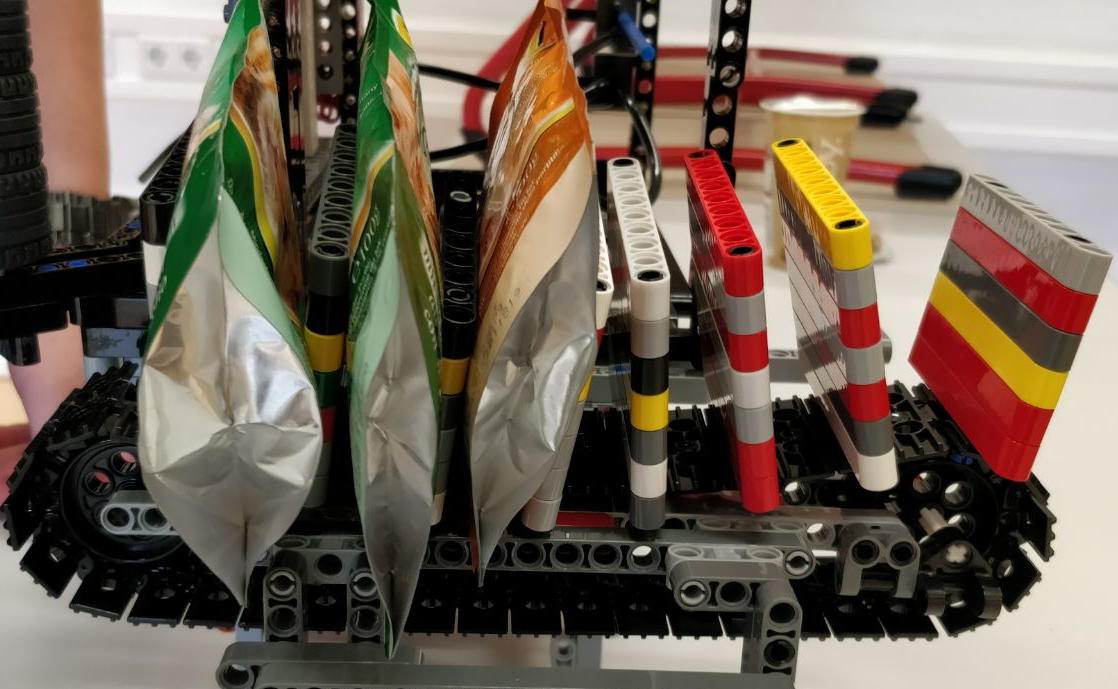
\includegraphics[width=1\textwidth]{Bilder/Ablauf_1_png/Magazin_Seitlich}
      \caption{Magazin Modellaufbau von der Seite}
      \label{Magazin Seitlich}
   \end{minipage}
   \hspace{.04\linewidth}% Abstand zwischen Bilder
   \begin{minipage}[hbt]{0.5\textwidth} % [b] => Ausrichtung an \caption
      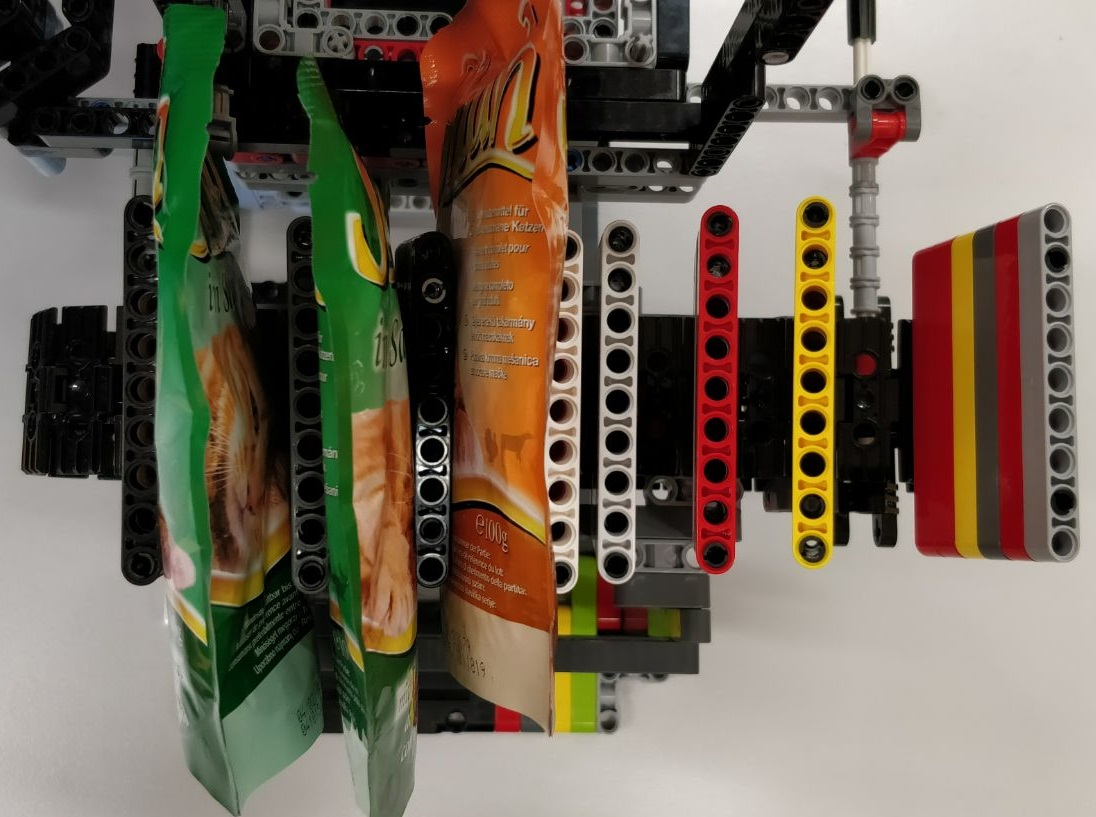
\includegraphics[width=0.92\textwidth]{Bilder/Ablauf_1_png/Magazin_Oben}
      \caption{Magazin Modellaufbau von Oben}
	  \label{Magazin Oben}      
      \end{minipage}
\end{figure}



\subsubsection{Führen zur Schneidplatte}

In diesem Schritt wird mithilfe eines Greifers (dargestellt durch eine Hand) die Packung in richtiger Position gebracht.
Durch die richtige Höhe des Förderbandes muss der Greifer keine hohe Kraft aufwenden, um die Packung an ihrem Zielort zu bringen. Der Greifer dient auch noch dazu, während des Schneidens neben den Magnetzylindern die Packung stabil zu positionieren und zu fixieren , ohne dass der Schnittpunkt verrutscht und die Schneide nicht mehr die Einkerbung, die leichter zu Schneiden ist, trifft. Eine schlechte Fixierung kann zu dem Problem führen, dass man die dickere Kunstoffumhüllung schneidet und der Schnitt nicht Ordnungsgemäß durchgeführt wird. Dadurch kann der Kunstoff zwischen die Schneiden gelangen und diese damit auseinander drücken. Dadurch würde dann die Packung nicht aufgeschnitten werden können. Nur bei sehr guter Einspannung tritt beim Schnitt eine Schubbelastung auf, die einen relativ geringen Kraftaufwand für die Rissfortpflanzung erfordert. Die ertragbare Schubspannung muss immer nur punktuell in der Risskerbe überschnitten werden. Bei schlechter Einspannung besteht die Gefahr, dass die Zugspannung über einen größeren Bereich auftreten würde, was enorme Kräfte erfordern würde. Siehe Abbildungen: \ref{Magazin Auszug}, \ref{Magazin Mitte}

\begin{figure}[H]
   \begin{minipage}[hbt]{0.5\textwidth} % [b] => Ausrichtung an \caption
      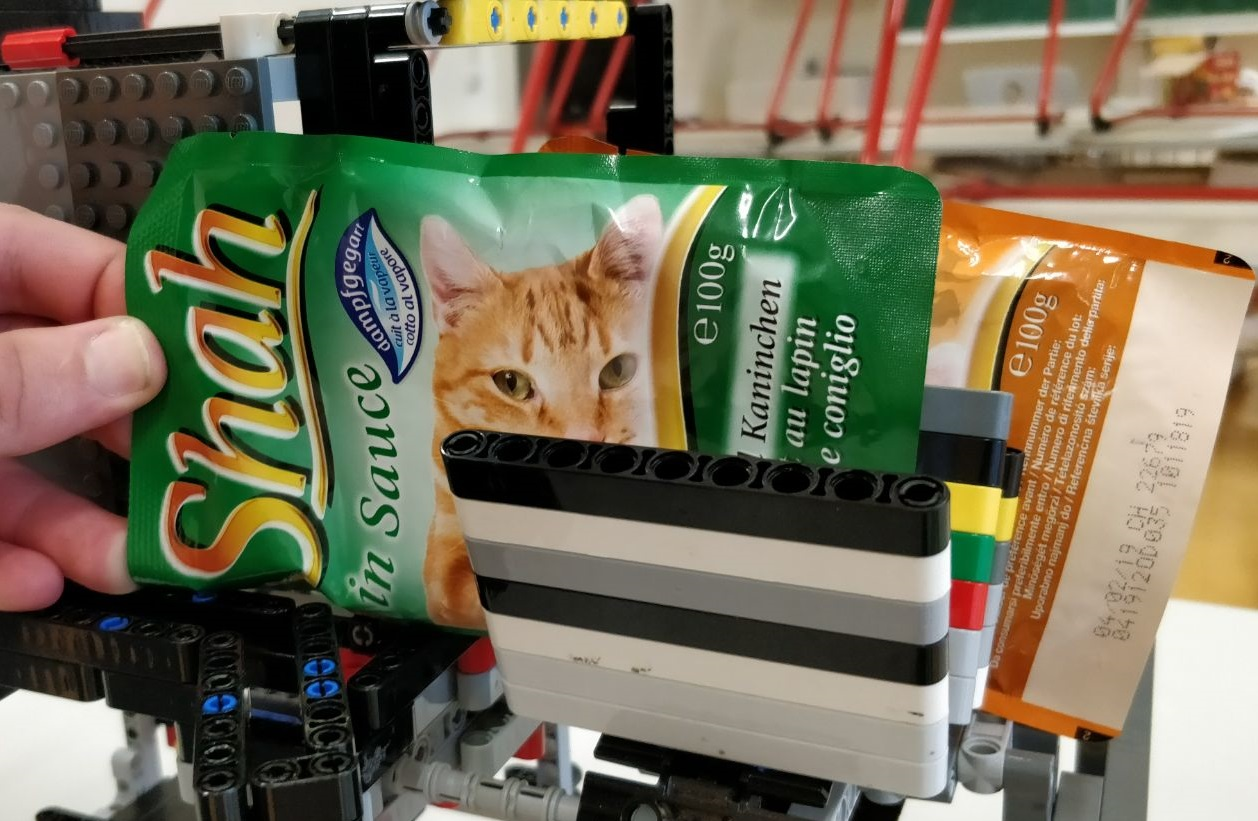
\includegraphics[width=1\textwidth]{Bilder/Ablauf_1_png/Magazin_Auszug}
      \caption{Magazin Auszug}
      \label{Magazin Auszug Start}
   \end{minipage}
   \hspace{.04\linewidth}% Abstand zwischen Bilder
   \begin{minipage}[hbt]{0.5\textwidth} % [b] => Ausrichtung an \caption
      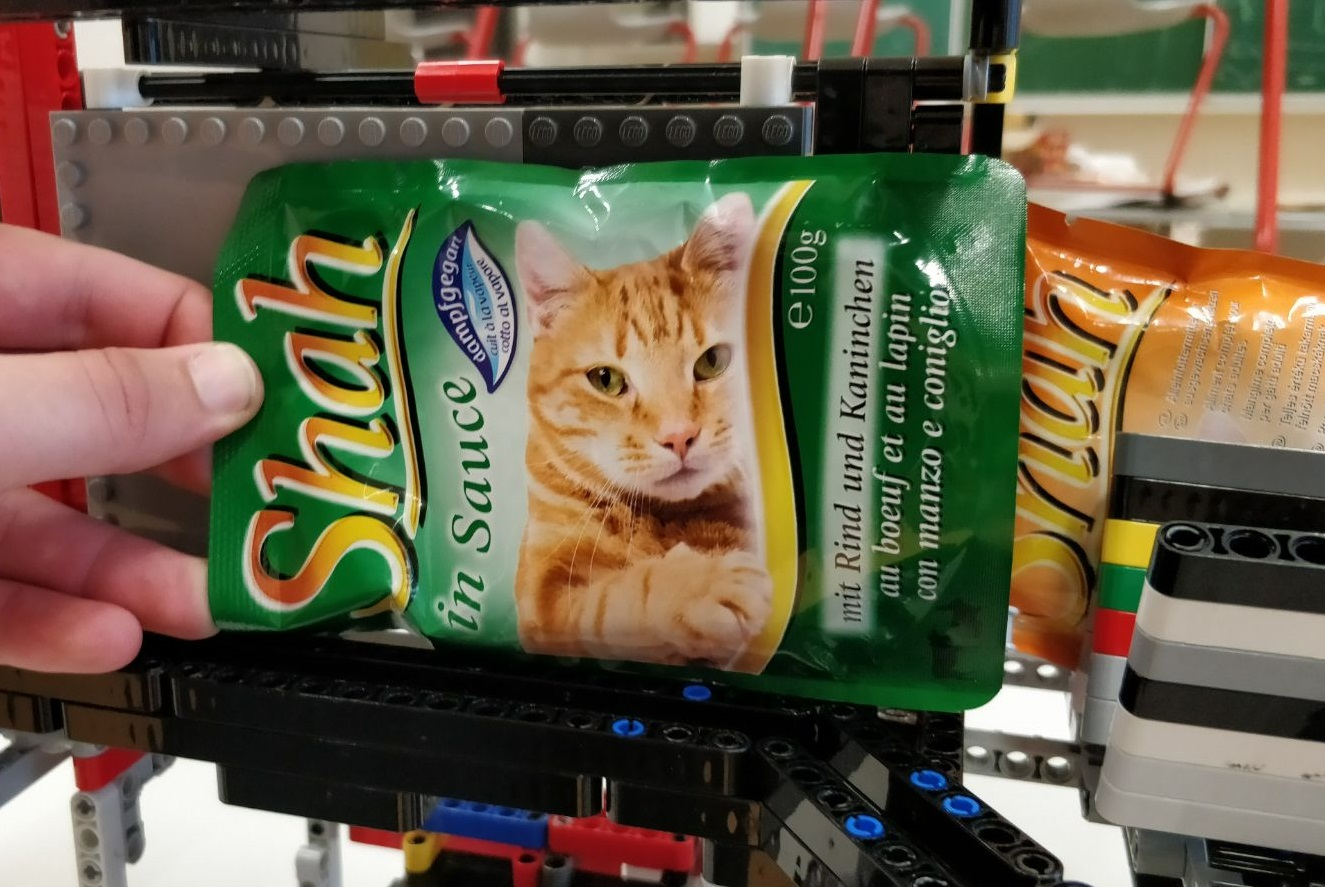
\includegraphics[width=0.92\textwidth]{Bilder/Ablauf_1_png/Magazin_Auszug_2}
      \caption{Magazin Auszug Mitte}
	  \label{Magazin Mitte}      
      \end{minipage}
\end{figure}

\vspace{20pt}

\begin{wrapfigure}{r}{0.5\textwidth}
\vspace{-30pt}
  \begin{center}
    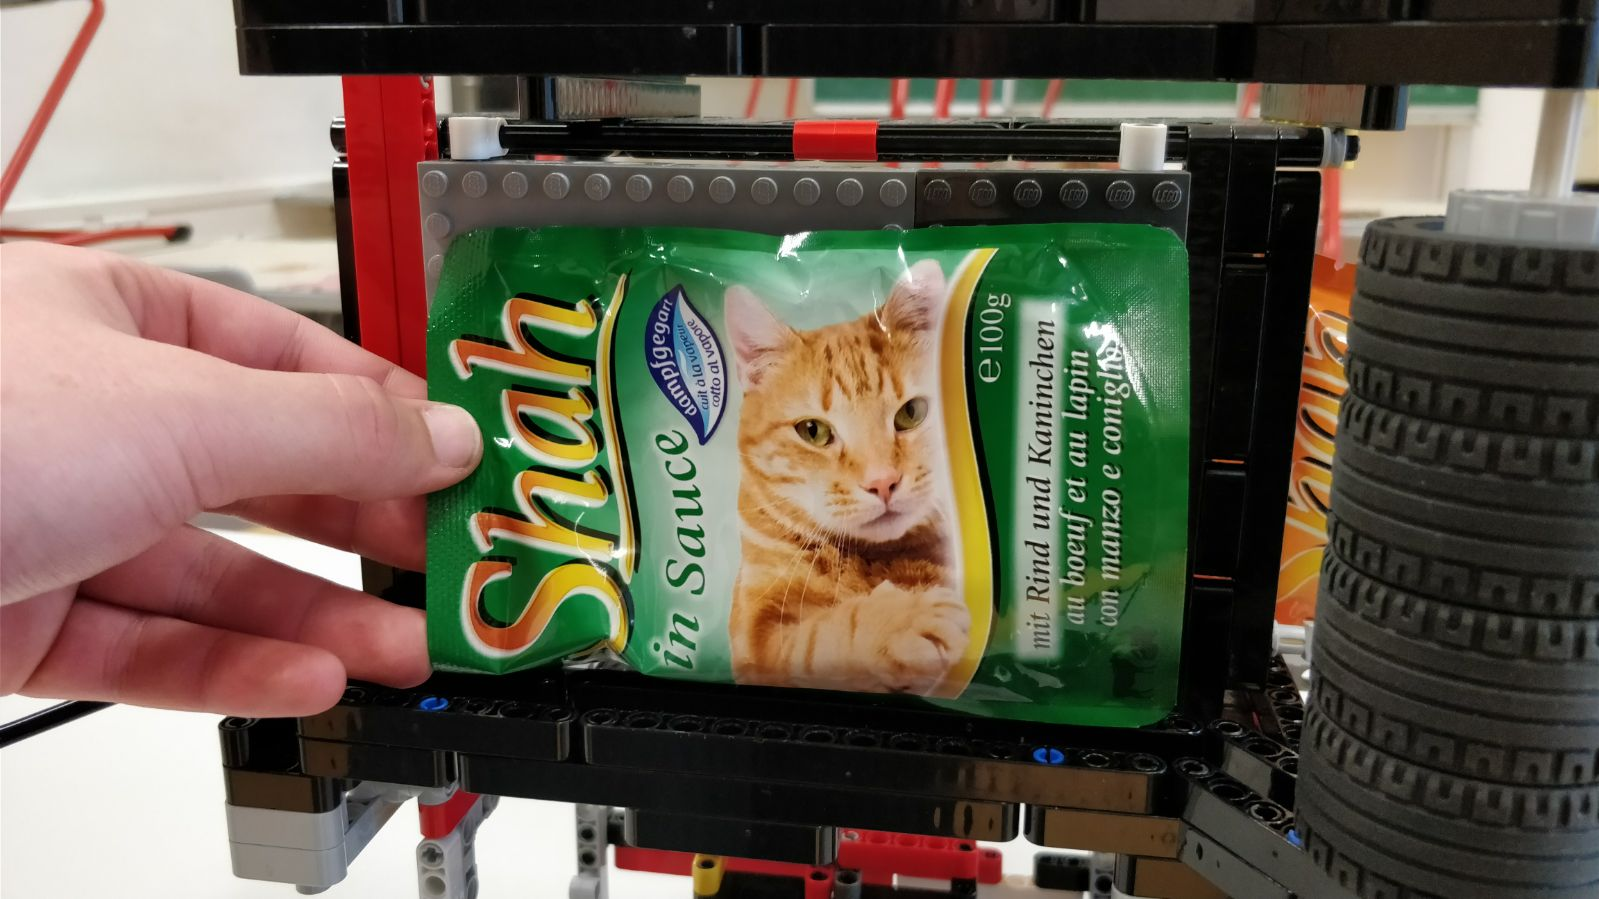
\includegraphics[width=0.50\textwidth]{Bilder/Ablauf_1_png/Schneidebereit}
  \end{center}
  \caption{Schneidebereit}
  \label{Schneidebereit}
  \vspace{-10pt}
\end{wrapfigure}

Wie im Bild \ref{Schneidebereit} gezeigt liegt das Katzenfutterpackerl in der richtigen Position und wird mit zwei Magnetzylindern an der Schneidefläche festgehalten. Die Magnetzylinder haben genügend Kraft, um die Packung auch während des Schnittes und der Walzphase in Position zu halten. Wenn die Packung verrutschen würde, könnte im schlimmsten Fall die Funktion der Maschine beeinflusst werden, indem sie den Greifer oder das Förderband blockiert. Daraufhin müsste die Maschine manuell geöffnet und der Beutel per Hand raus geholt werden.
\subsubsection{Schnitt}

\begin{wrapfigure}{r}{0.5\textwidth}
\vspace{-30pt}
  \begin{center}
    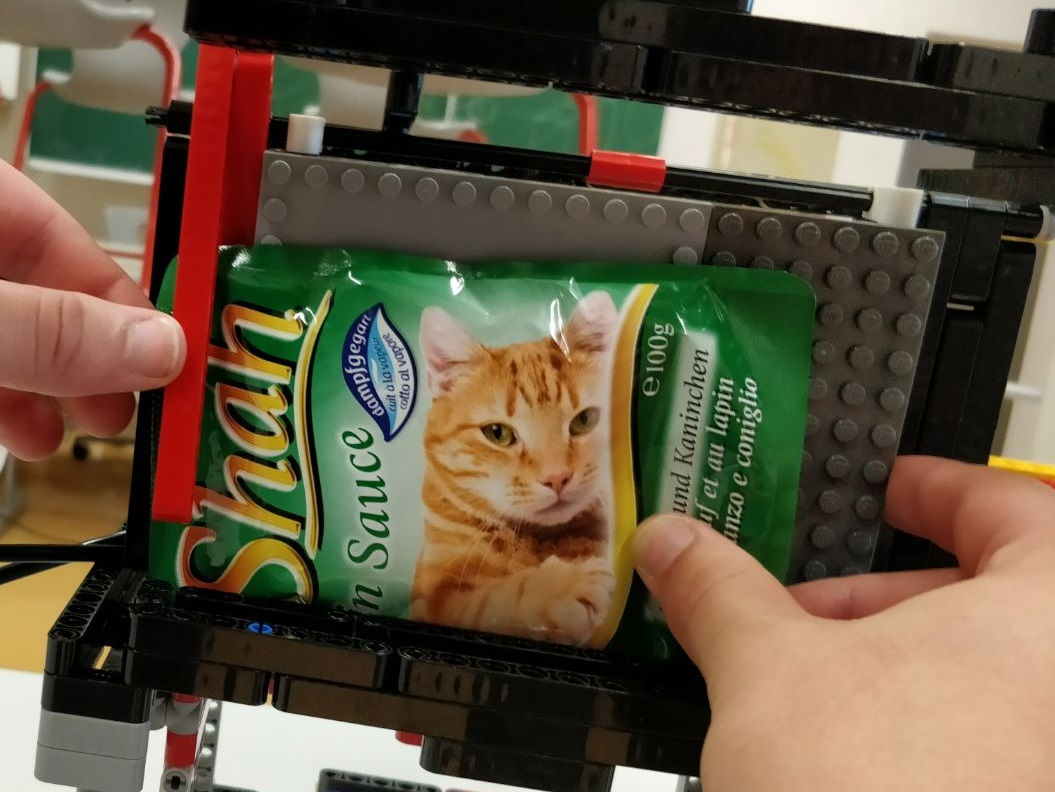
\includegraphics[width=0.50\textwidth]{Bilder/Ablauf_1_png/Schnitt}
  \end{center}
  \caption{Schnitt}
  \label{Schnitt}
  \vspace{-10pt}
\end{wrapfigure}

In der richtigen Position muss man mit zwei scharfen Klingen mit viel Kraft die Packung aufschneiden. Eine davon wird an der Schnittfläche angebracht und die andere macht die Schneidbewegung, wobei die beiden aneinander reibenden Kanten den Schnitt verursachen. Die Packung kann mit einem Schnitt vollständig geöffnet werden. Mit zu wenig Druck zwischen den Klingen gelangt zu viel Kunstoffmaterial zwischen die Schneideflächen und durch die Länge der Schneiden biegen sie sich auseinander und somit würde  kein ordentlicher Schnitt entstehen (Zugspannung statt örtliche Schubspannung). Mehrmaliges Auftreten dieses beschriebenen Problems bei der selben Packung kann es zufolge haben, dass sich die Packung nicht mehr mit der Maschine schneiden lässt, weil sie sich durch die vielen Versuche verformt hat. Da die Maschine nicht erkennt ob der Schnitt erfolgreich war würde die Katze bei misslungenem Schnitt nicht gefüttert werden. Siehe Abbildung: \ref{Schnitt} \\

Eine Alternative wäre ein feingezähntes Schneiderad mit hoher Drehzahl. Versuche mit einem gezähnten Messer haben gezeigt, dass etwa neun Schnitte mit einem Messer, erforderlich waren um eine Verpackung vollständig aufzuschneiden. Für genauer Informationen siehe \ref{Schneideversuch_2}


\subsubsection{Pressen}

\begin{wrapfigure}{r}{0.5\textwidth}
\vspace{-30pt}
  \begin{center}
    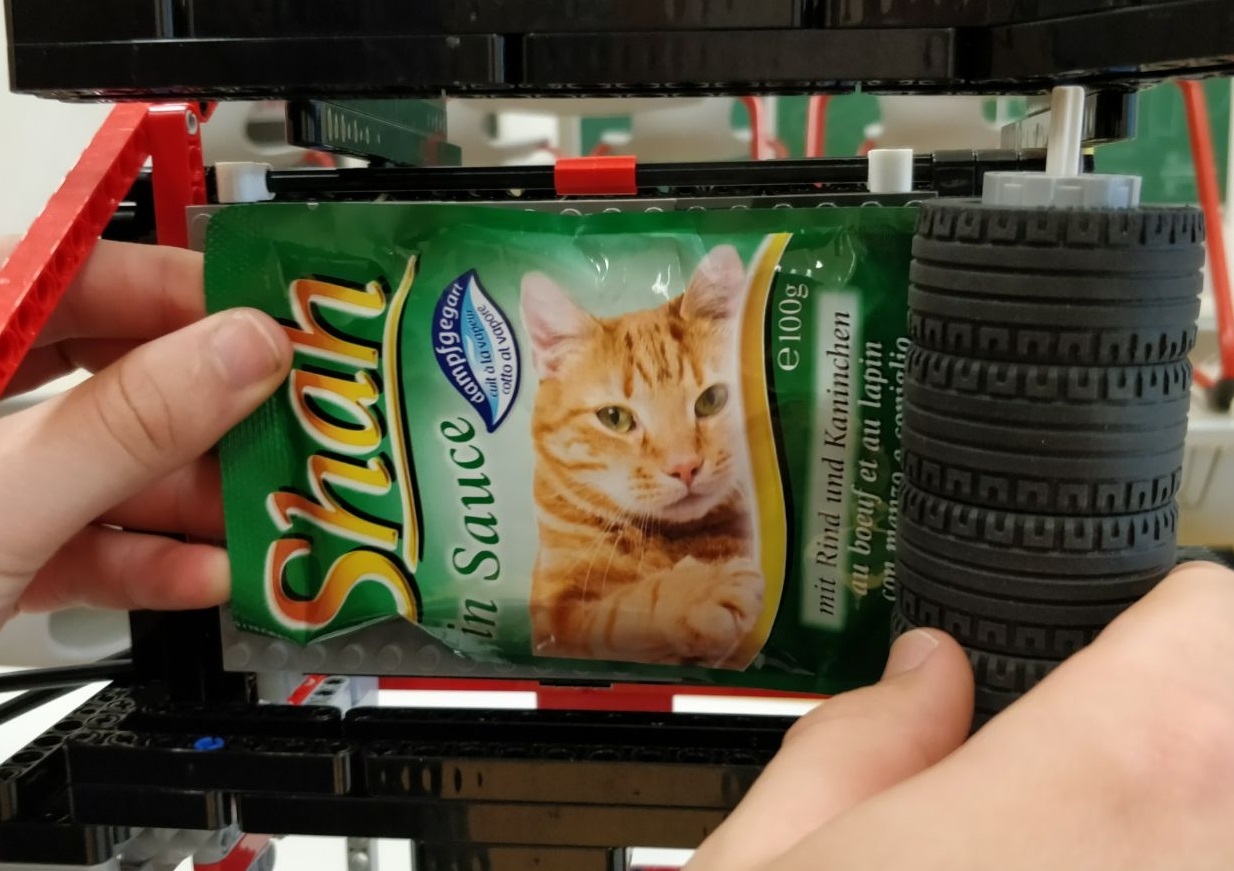
\includegraphics[width=0.50\textwidth]{Bilder/Ablauf_1_png/Ausquetschen_1}
  \end{center}
  \caption{Ausquetschen Beginn}
  \label{Ausquetschen Beginn}
  \vspace{-10pt}
\end{wrapfigure}

Nach dem Aufschneiden wird mit einer Rolle die Packung ausgepresst. Dazu werden zuerst die ersten zwei Magnetzylinder gelöst, bis sich die Rolle vorbei bewegt hat. Danach werden sie wieder in Position gebracht. Daraufhin werden die anderen beiden gelöst und die Rolle fährt ans Ende. Die Rolle ist auf einer Welle platziert, diese wird mit zwei Sicherungsringen an einer  vorgegebenen Position befestigt. Die Rolle ist 10 cm breit, damit ohne Probleme die 9,4cm breite Futterpackung ausgepresst werden kann. Sie wird in einer Vorrichtung an der Maschine angehängt und steht mit einem bestimmten Winkel auf die Schneidfläche damit ein großer Anpressdruck entsteht. Durch die schmierige Konsistenz gleitet das Futter aus der Verpackung und wird nicht von der Walze zerquetscht. Nach der Beseitigung der Verpackung werden zuerst die beiden Magnetzylinder von der Maschine entfernt in Anfangsposition gebracht, damit die Walze ohne Probleme in Startposition zurückkehren kann. Siehe Abbildungen: \ref{Ausquetschen Beginn}, \ref{Ausquetschen Mitte}, \ref{Ausquetschen Ende}



\begin{figure}[H]
   \begin{minipage}[hbt]{0.5\textwidth} % [b] => Ausrichtung an \caption
      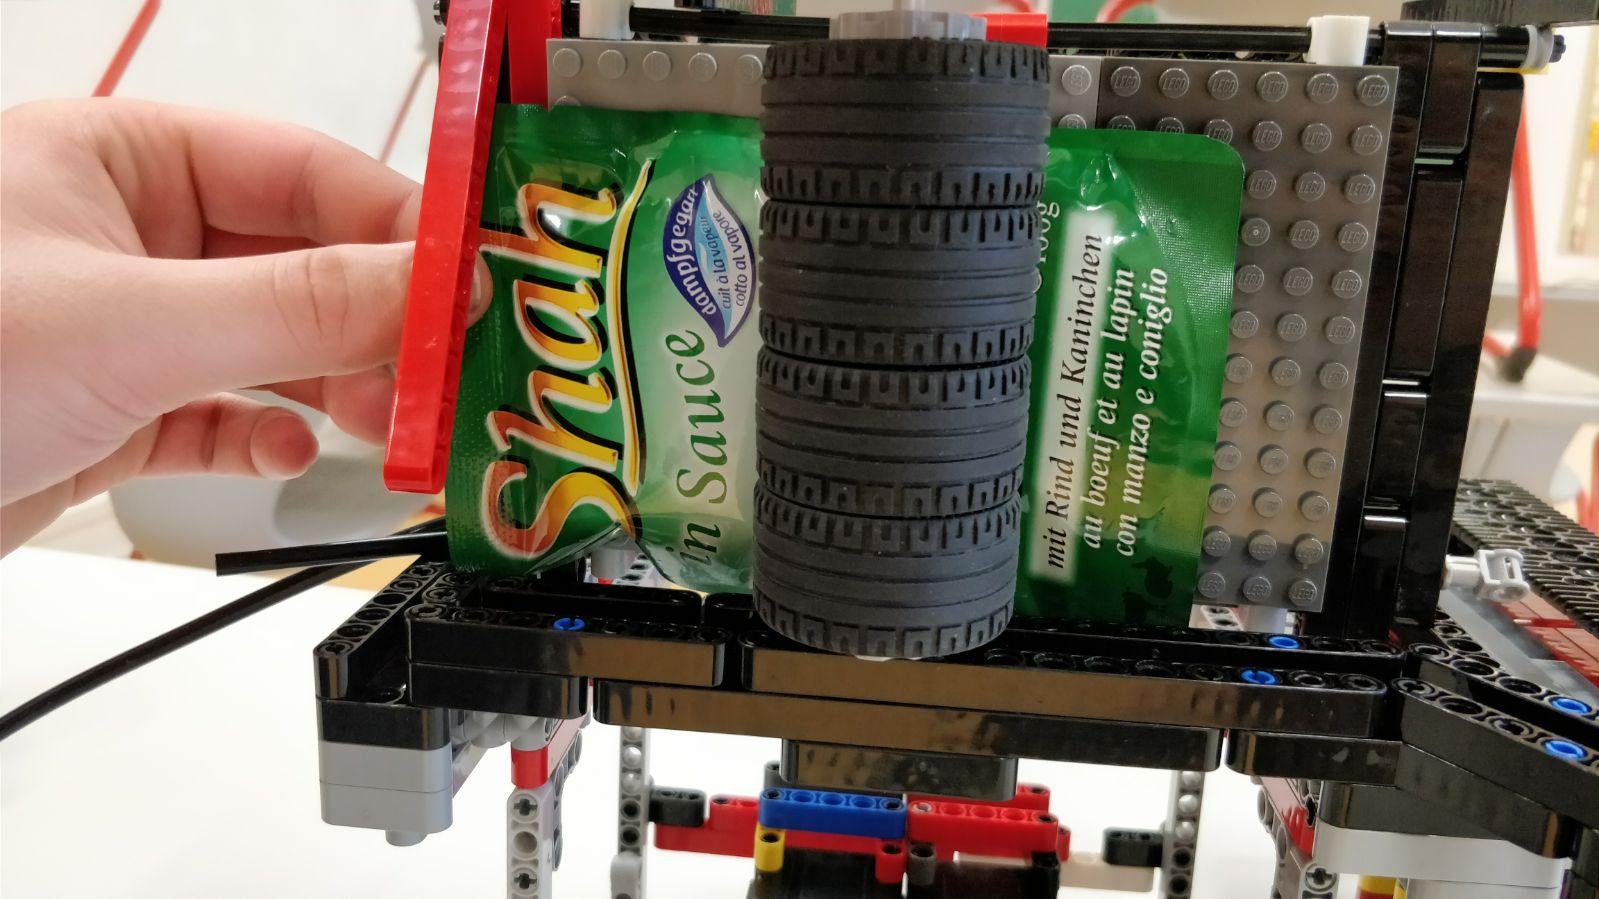
\includegraphics[width=1\textwidth]{Bilder/Ablauf_1_png/Ausquetschen_2}
      \caption{Ausquetschen Mitte}
      \label{Ausquetschen Mitte}
   \end{minipage}
   \hspace{.04\linewidth}% Abstand zwischen Bilder
   \begin{minipage}[hbt]{0.5\textwidth} % [b] => Ausrichtung an \caption
      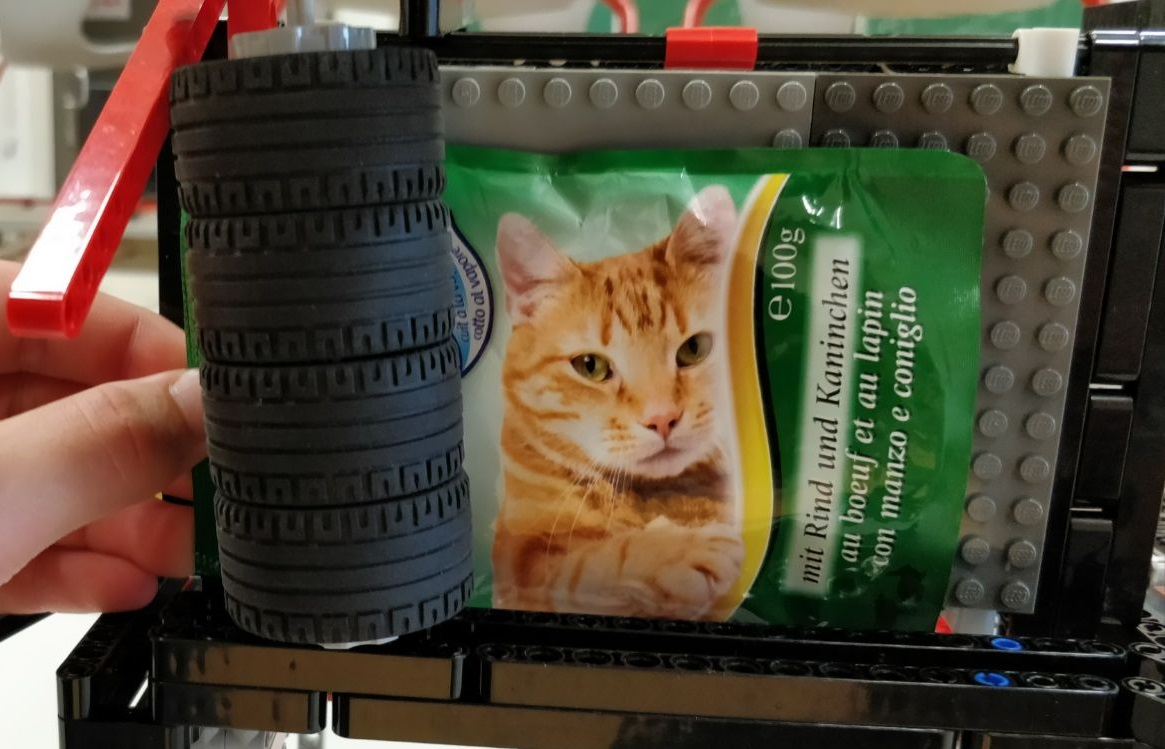
\includegraphics[width=0.98\textwidth]{Bilder/Ablauf_1_png/Ausquetschen_3}
      \caption{Ausquetschen Ende}
	  \label{Ausquetschen Ende}      
      \end{minipage}
\end{figure}

Eine Alternative wäre ein senkrechtes Ausquetschen nach unten, unterstützt von der Schwerkraft. Dies ist bei dieser Variante schwer zu realisieren.

\subsubsection{Entsorgen}

\begin{wrapfigure}{r}{0.5\textwidth}
\vspace{-30pt}
  \begin{center}
    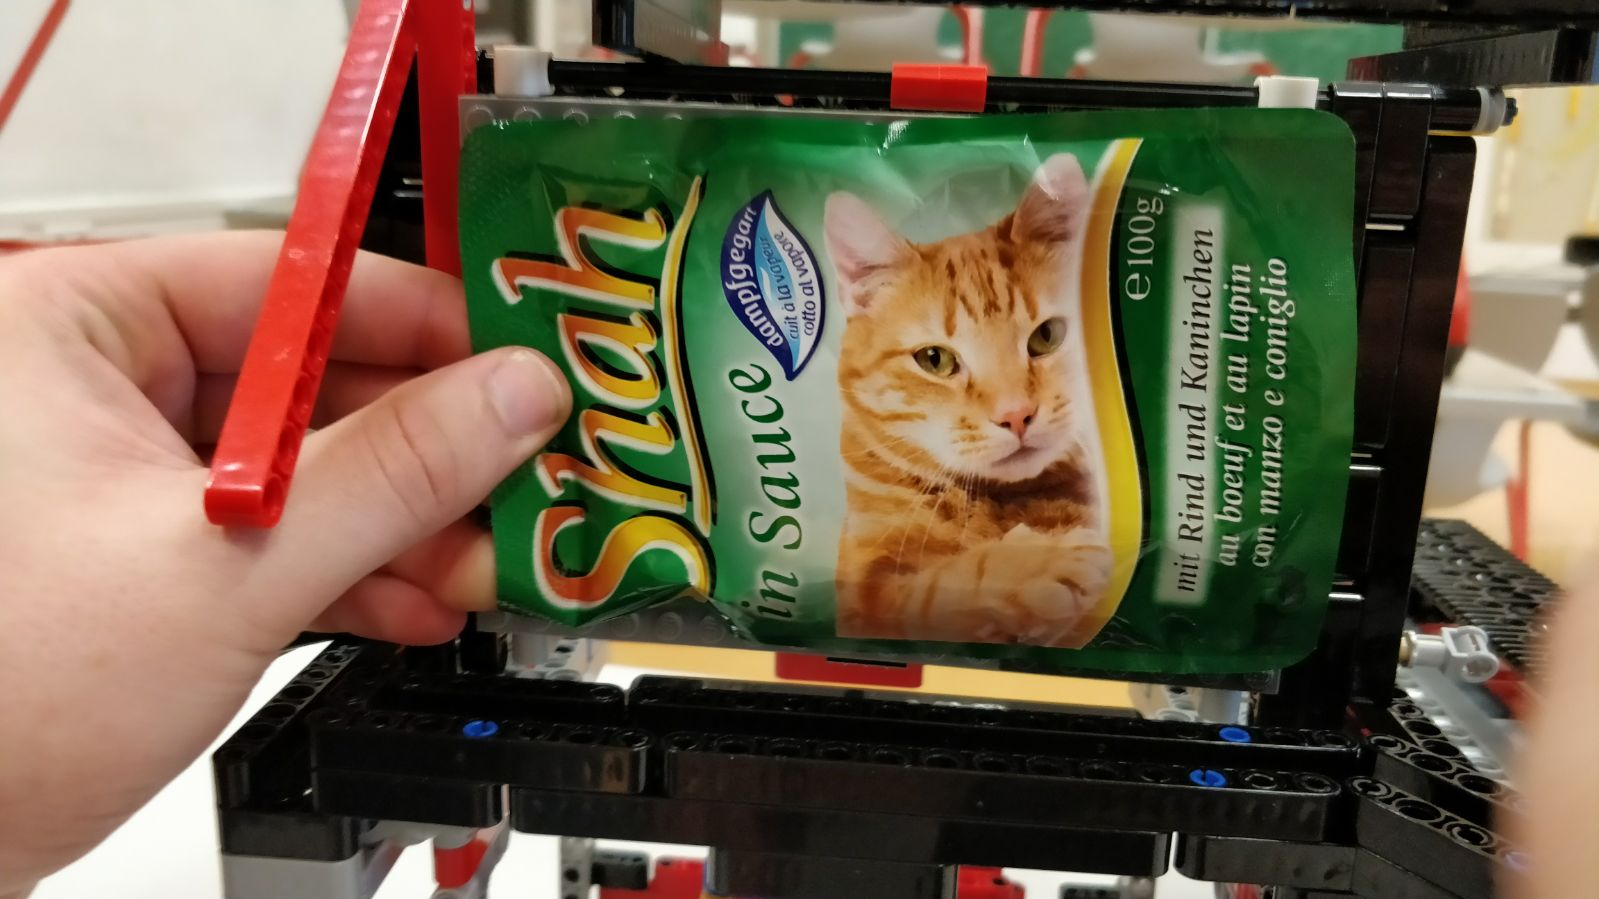
\includegraphics[width=0.50\textwidth]{Bilder/Ablauf_1_png/Auswurf_1}
  \end{center}
  \caption{Auswurf Beginn}
  \label{Auswurf Beginn}
  \vspace{-10pt}
\end{wrapfigure}

Nach dem Auspressen wird die leere Packung durch die Rückklappe in einen Luftdichten Container geworfen. Die Klappe wird durch zwei Stifte gehalten und lässt sich durch ein Scharnier nach hinten klappen. Die zwei Stifte sind mit Kosten verbunden, da zwei Magnetzylinder benötigt werden und diese auch, in einem Schaltplan zu berücksichtigen sind. Außerdem benötigen sie zusätzlich Platz. Die Klappe befindet sich hinter der Futterverpackung. Siehe Abbildung: \ref{Auswurf Beginn}. \\

In Abbildung: \ref{Bolzen drinnen} sieht man den Stift (oranger Kreis) der ein vorzeitiges nach Hinten klappen verhindert. Die Stifte müssen so dimensioniert sein, dass sie die Kräfte der Walze aushalten. \\

In Abbildung: \ref{Bolzen entfernen} wurde der Bolzen entfernt (oranger Kreis) und somit lässt sich die Klappe nach hinten klappen. 

\begin{figure}[H]
   \begin{minipage}[hbt]{0.5\textwidth} % [b] => Ausrichtung an \caption
      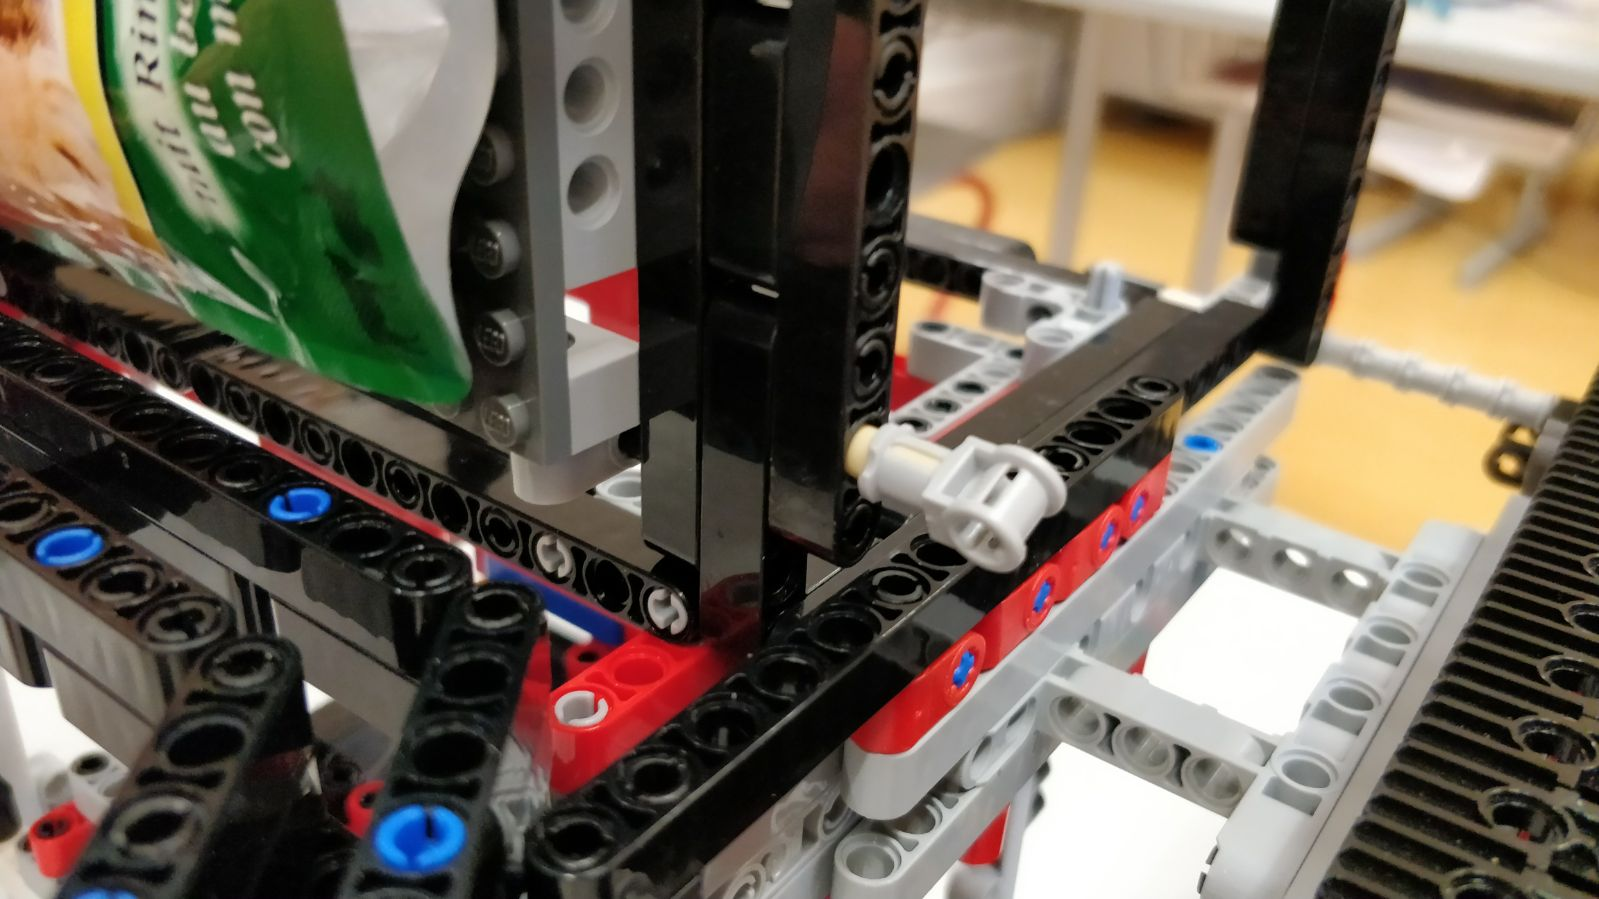
\includegraphics[width=1\textwidth]{Bilder/Ablauf_1_png/Auswurf_2}
      \caption{Bolzen drinnen}
      \label{Bolzen drinnen}
   \end{minipage}
   \hspace{.04\linewidth}% Abstand zwischen Bilder
   \begin{minipage}[hbt]{0.5\textwidth} % [b] => Ausrichtung an \caption
      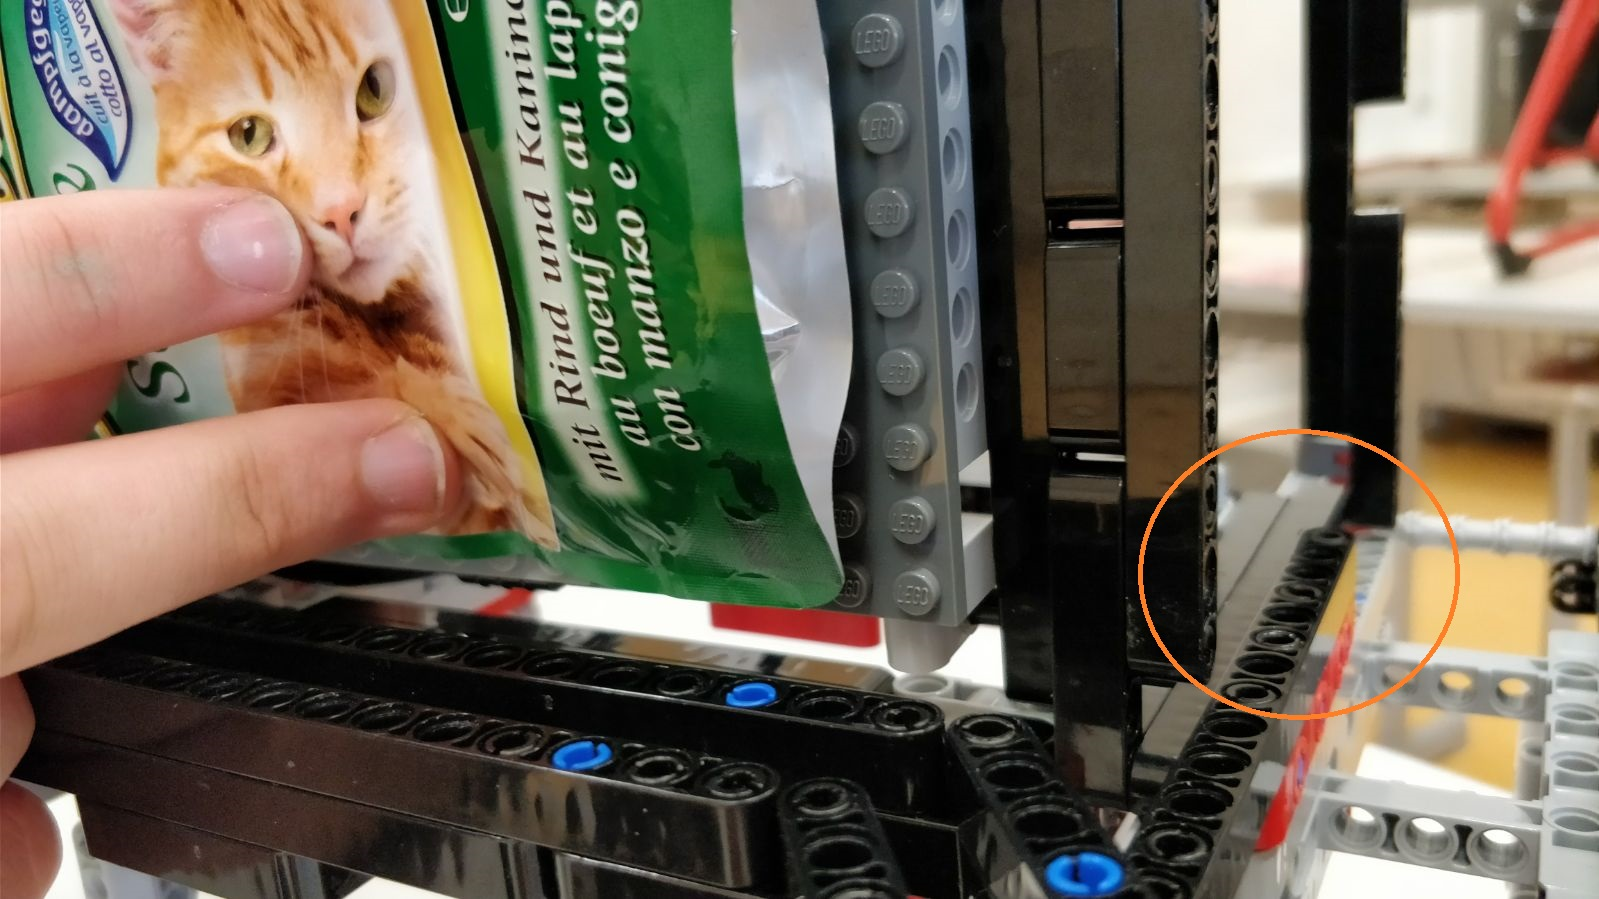
\includegraphics[width=1\textwidth]{Bilder/Ablauf_1_png/Auswurf_3}
      \caption{Bolzen entfernen}
	  \label{Bolzen entfernen}      
      \end{minipage}
\end{figure}


In Abbildung: \ref{Klappe öffnen} wird demonstriert wie die Magnetzylinder die leere Packung gegen die Klappe drücken, wodurch die Klappe sich öffnet und die leere Packung hinunterfällt.\\

In Abbildung: \ref{Fertiger Auswurf} sieht man sehr gut, wie die Klappe aussieht und wie sie nach hinten aufgeht und der Futtersack in der luftdichten Box entsorgt wird.


\begin{figure}[H]
   \begin{minipage}[hbt]{0.5\textwidth} % [b] => Ausrichtung an \caption
      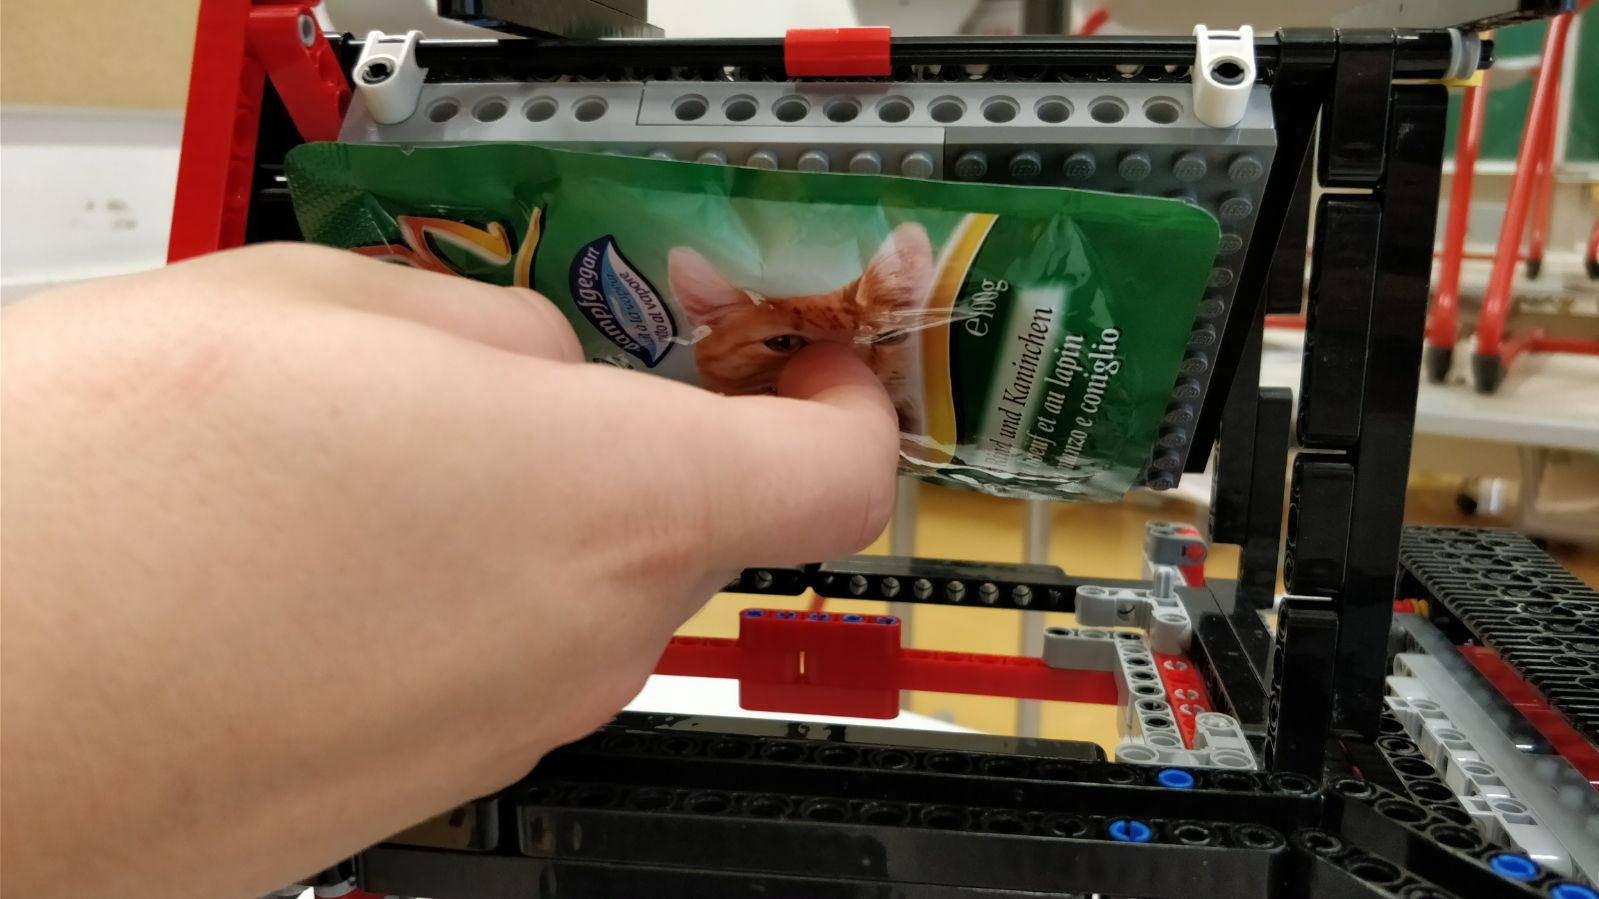
\includegraphics[width=1\textwidth]{Bilder/Ablauf_1_png/Auswurf_4}
      \caption{Klappe öffnen}
      \label{Klappe öffnen}
   \end{minipage}
   \hspace{.04\linewidth}% Abstand zwischen Bilder
   \begin{minipage}[hbt]{0.5\textwidth} % [b] => Ausrichtung an \caption
      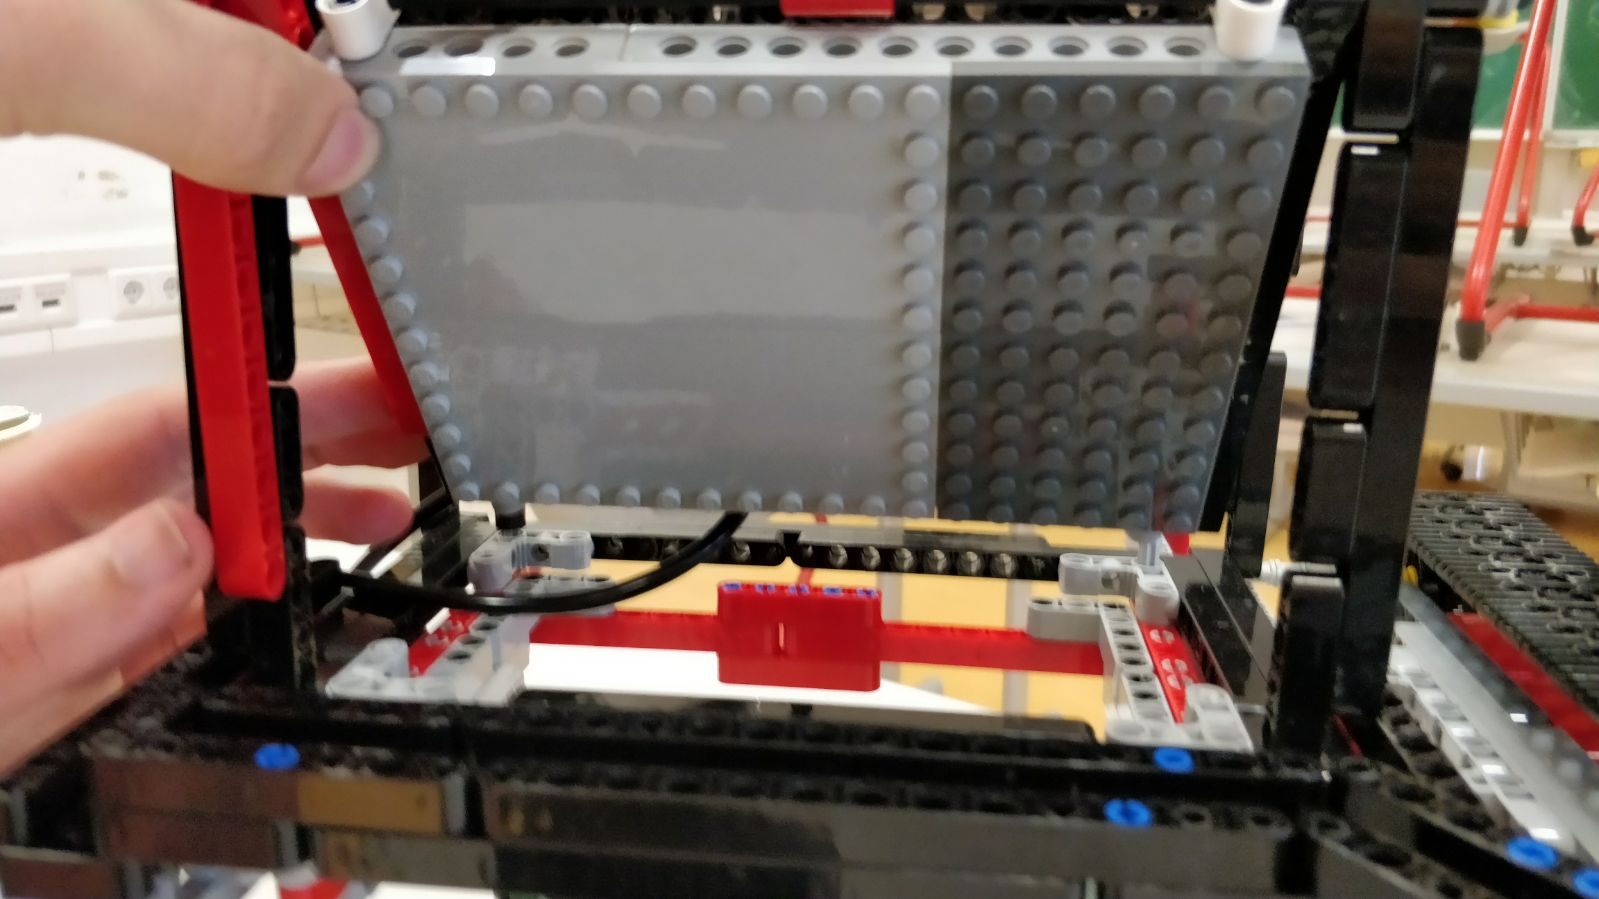
\includegraphics[width=1\textwidth]{Bilder/Ablauf_1_png/Auswurf_5}
      \caption{Fertiger Auswurf}
	  \label{Fertiger Auswurf}      
      \end{minipage}
\end{figure}


\subsubsection{Füttern}

\begin{wrapfigure}{r}{0.5\textwidth}
\vspace{-40pt}
  \begin{center}
    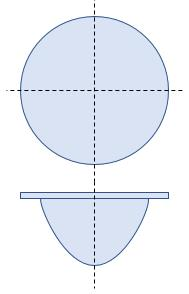
\includegraphics[width=0.17\textwidth]{Bilder/Powerpoint/Loch_Futterschuessel}
  \end{center}
  \caption{Einhänge Futterschüssel}
  \label{Loch_Futterschuessel}
  \vspace{-10pt}
\end{wrapfigure}

Die Maschine besitzt fünf Futterschüsseln die auf einer drehbaren Platte stehen. Vor dem Füttern wird eine saubere Platte unter der Stelle, wo später die Packung aufgeschnitten wird, positioniert. Während es ausgepresst wird, fällt das Futter in die Futterschüssel. Wenn der Auspressvorgang beendet ist, wird die Futterschüssel an eine Position bewegt, wo die Katze Zugang zum fressen hat. Die Schüsseln lassen sich einfach aus der Halterung nehmen, da sie nur in einem Loch in der Platte liegen. Das hat den Vorteil gegenüber anderen Schüsseln die auf der Platte montiert sind, dass die Schüssel rasch und eindeutig positioniert werden kann und die Katze nicht soweit zur Futterschüssel hat. Die Platte ist mit einer Gummischicht überzogen damit die Schüssel, durch der Kopf der Katze, wenn sie frisst, nicht verrutscht. Sie lässt sich aus der Platte entnehmen, indem der Benutzer mit der Hand die Futterschüssel von unten durch das Loch drückt und mit der anderen Hand entnimmt. Danach werden die Schüsseln gewaschen, getrocknet und danach in das Loch fallen gelassen. Siehe Abbildung: \ref{Loch_Futterschuessel}

\subsection{Variante 2: Vor aufgeschnittene Packung }

Diese Variante wurde entwickelt um den Schneidemechanismus zu umgehen, da das Schneiden kein leichtes Unterfangen ist. Hierbei wird jedoch dem Benutzer zugemutet, mehr Zeit in die Maschine zu investieren als bei den anderen Varianten. Er muss sämtliche Packungen aufschneiden mit einer Klemme versehen und in das Förderband einhängen. Mit dieser Bauweise wird viel auf die Hilfe der physikalischen Kräfte gesetzt. Die Schwerkraft wird maßgeblich genutzt um die Packung zu entleeren.

\subsubsection{Förderband und Kettenglieder}

Für das Förderband wird über die zwei Kettenräder eine Kette gespannt. Auf diese Kette werden die Futterpackungen gehängt, dass funktioniert aber nur weil die Kettenglieder einen rechten Winkel auf jeder Seite haben (siehe Abbildung: \ref{Kettenglied}). Auf diesen Winkel wird eine Aluplatte geschraubt und mit einer anderen Platte festgeklemmt. Die Kette wird mithilfe eines Kettenrades und eines Motors in Bewegung gebracht, damit bewegt sich die Packung immer näher Richtung Walze. Da die Packung senkrecht auf das Förderband gehängt wird, spielt die Schwerkraft eine große Rolle und unterstützt den Entleerungsprozess der Katzenfutterpackung.\\ Die zwei dunkelblauen Kreise symbolisieren die zwei Kettenräder, die die Kette antreiben. Um die Kreise liegen die einzelnen Kettenglieder, verbunden zu einer Kette. Die Pfeile sollen die Futterpackungen darstellen, die am Schaft an der Kette befestigt sind und mit den Öffnungen(Pfeilspitzen) nach unten zeigen. Siehe Abbildung: \ref{Foerderband}. \\
Die dunklere von den blauen Flächen ist die Oberseite des rechten Winkels mit zwei Löchern zur Befestigung der Aluplatte. Die hellere Fläche ist die Unterseite des Winkels. Die Bolzen des Kettengliedes sind Orange eingezeichnet. Siehe Abbildung: \ref{Kettenglied}.

\begin{figure}[H]
   \begin{minipage}[hbt]{.3\linewidth} % [b] => Ausrichtung an \caption
      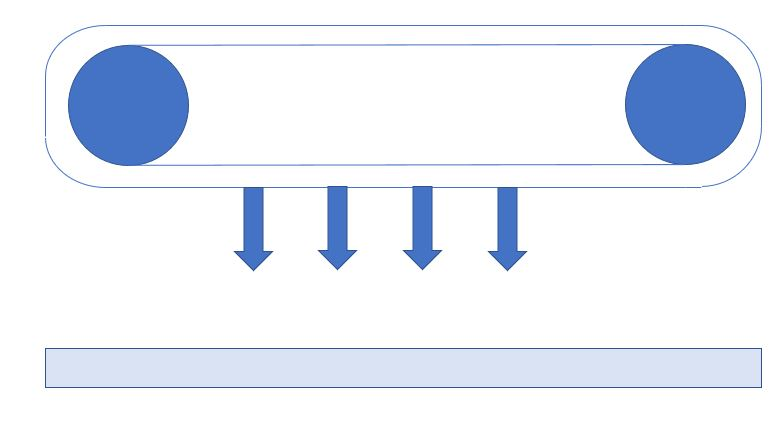
\includegraphics[width=\linewidth]{Bilder/Powerpoint/Foerderband}
      \caption{Foerderband}
      \label{Foerderband}
   \end{minipage}
   \hspace{.3\linewidth}% Abstand zwischen Bilder
   \begin{minipage}[hbt]{.3\linewidth} % [b] => Ausrichtung an \caption
      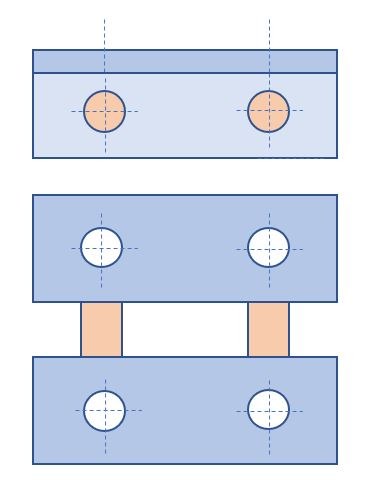
\includegraphics[width=\linewidth]{Bilder/Powerpoint/Kettenglied}
      \caption{Kettenglied}
	  \label{Kettenglied}      
      \end{minipage}
\end{figure}

\subsubsection{Walze}

Die Walze dient zum Ausquetschen der Futterpackung. Nachdem die Futterpackung in Bewegung ist, wird bei einer gewissen Position die Klemme entfernt und durch die Walze gepresst. Die Walze ist innen hohl und wird auf der Welle platziert. Die erste Walze auf der Antriebsseite und die zweite Walze auf einer eigenen gefertigten Welle. Beide Walzen werden durch eine Feder aneinander gepresst, nur so stark, dass die Halterung, an der die Packung festgemacht ist, durchkommt. Dennoch so stark, dass sich die Packung entleert. Die Walze an der eigen gefertigten Welle wird mit zwei Aluplatten und einem Scharnier in Stellung gehalten.\\ 
In Abbildungen: \ref{Walze} ist auf der Walze ein Pfeil gezeichnet. Der Pfeil stellt eine Futterpackung dar und die Pfeilrichtung zeigt die Richtung, in der die Packung ausgepresst wird.  \\
In Abbildungen: \ref{Scharnier}ist der dunkelblaue Teil das eigentliche Scharnier, die hellblauen Flächen sind die Verlängerungen. 

\begin{figure}[H]
   \begin{minipage}[hbt]{.4\linewidth} % [b] => Ausrichtung an \caption
      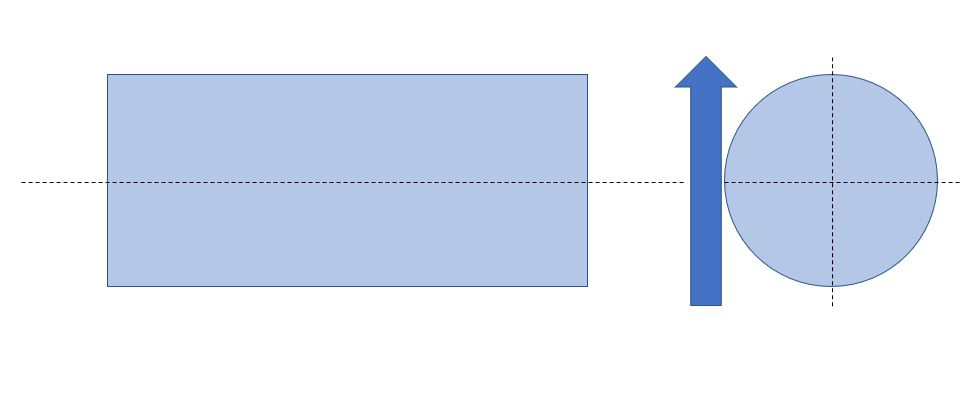
\includegraphics[width=\linewidth]{Bilder/Powerpoint/Walze}
      \caption{Walze}
      \label{Walze}
   \end{minipage}
   \hspace{.2\linewidth}% Abstand zwischen Bilder
   \begin{minipage}[hbt]{.4\linewidth} % [b] => Ausrichtung an \caption
      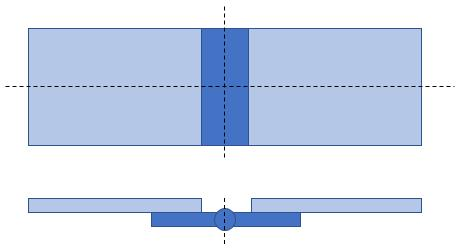
\includegraphics[width=\linewidth]{Bilder/Powerpoint/Schanier}
      \caption{Scharnier}
	  \label{Scharnier}      
      \end{minipage}
\end{figure}
\newpage
\subsubsection{Futterplatte}

\begin{wrapfigure}{r}{0.5\textwidth}
\vspace{-30pt}
  \begin{center}
    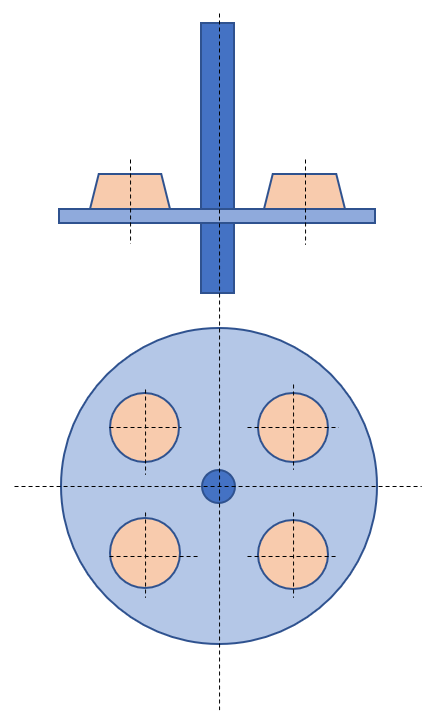
\includegraphics[width=0.20\textwidth]{Bilder/Powerpoint/Futterplatte}
  \end{center}
  \caption{Futterplatte}
  \label{Futterplatte}
  \vspace{-20pt}
\end{wrapfigure}


Nach dem Pressen wird das Futter in die Schüssel gequetscht bzw. es rinnt in die Schüssel. Die Platte hat je nach Bedarf eine gewisse Anzahl an Schüsseln, aber maximal fünf Schüsseln. Diese sind auf einer Platte platziert. Durch den Plattenmittelpunkt geht eine vertikale Welle, die die Platte nach links oder rechts drehen kann. Siehe Abbildung: \ref{Futterplatte} \\


\subsection{Variante 3: Gefrorenes Futter}

In dieser Variante wurde überlegt, das Futter einzufrieren, dieses danach aus der Gefriertruhe zu holen und zu erwärmen. Der Vorteil hierbei ist, dass keine Bakterien in das Futter gelangen können da es tiefgefroren ist und es kann die Portionsgröße beliebig eingestellt werden. Des weiteren müsste man nicht über das Schneide-Problem nachdenken, da es eine knifflige Angelegenheit ist, die Packung bei jeden Schnitt perfekt zu schneiden. Der große Nachteil ist der Platzbedarf und der hohe Energieverbrauch der Kühltruhe. Auch die Entnahme des Futters aus der Kühltruhe ist kein leichtes Unterfangen. Erstens kann mit Magnetzylindern gearbeitet werden, zur Verschiebung der Abdeckung. Zweitens könnte ein Loch in die Gefriertruhe geschnitten werden aus dem der Greifer das Futter entnimmt und darum wieder dicht halten muss. Falls es undicht ist, wird es darin zu warm, das Futter schmilzt und verdirbt schlussendlich. Hinzuzufügen ist auch noch, dass Katzen, wenn es um Futter, geht sehr wählerisch sind. Wenn das Futter gefroren ist, hat man zu einem  Teil das Kondenswasser des aufgetauten Futters und zum Anderen schmeckt eingefrorenes Essen anders, also nicht so wie es die Katze gewohnt ist.

\section{Aufbauten und Tests}

In diesem Abschnitt der Diplomarbeit wurden Teile der vorne beschriebenen Varianten aufgebaut und verschiedene Tests durchgeführt, um die Funktionalität der Varianten zu gewährleisten. \\

\subsection{Fütterungsexperiment} 

In diesem Experiment wurde getestet wie lange es dauert bis eine Packung nur mit Hilfe der Schwerkraft ausläuft. Der Beutel wurde nicht extra erwärmt und wurde nur an den beiden unteren Ecken gehalten. Siehe Abbildungen: \ref{Halterung}, \ref{Fütterungs Anfang} 

In Abbildung: \ref{Fütterungs Mitte} wird gezeigt wie viel nach 5 Minuten von der Packung in den Futterbehälter geflossen ist.

In Abbildung: \ref{Fütterungs_Ende} sieht man, dass nach 10 Minuten der ganze Inhalt in der Futterschüssel entleert wurde, dennoch Tropft es nach.


\begin{figure}[H]
   \begin{minipage}[hbt]{.4\linewidth} % [b] => Ausrichtung an \caption
      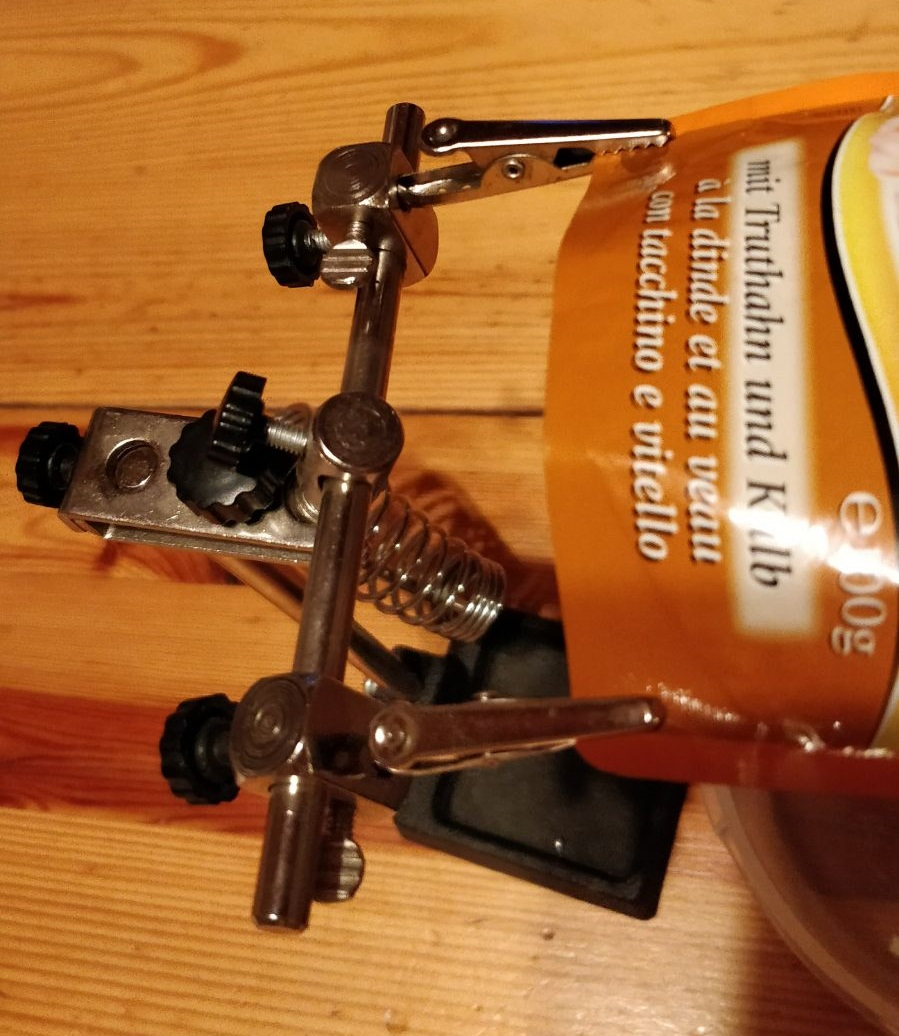
\includegraphics[width=\linewidth]{Bilder/Fuetterungsexperiment/Aufhaengung}
      \caption{Halterung}
      \label{Halterung}
   \end{minipage}
   \hspace{.2\linewidth}% Abstand zwischen Bilder
   \begin{minipage}[hbt]{.4\linewidth} % [b] => Ausrichtung an \caption
      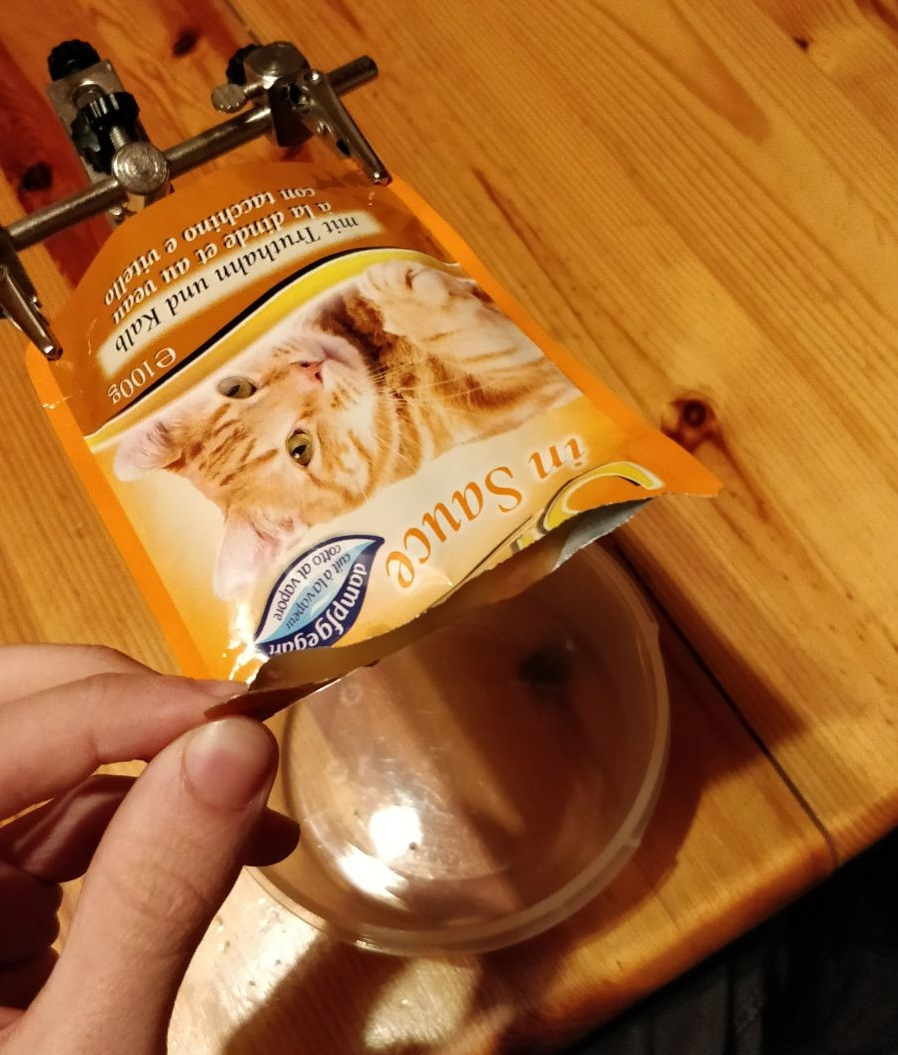
\includegraphics[width=\linewidth]{Bilder/Fuetterungsexperiment/Fuetterungs_Anfang}
      \caption{Entleerung Anfang}
	  \label{Fütterungs Anfang}      
      \end{minipage}
\end{figure}


\begin{figure}[H]
   \begin{minipage}[hbt]{.32\linewidth} % [b] => Ausrichtung an \caption
      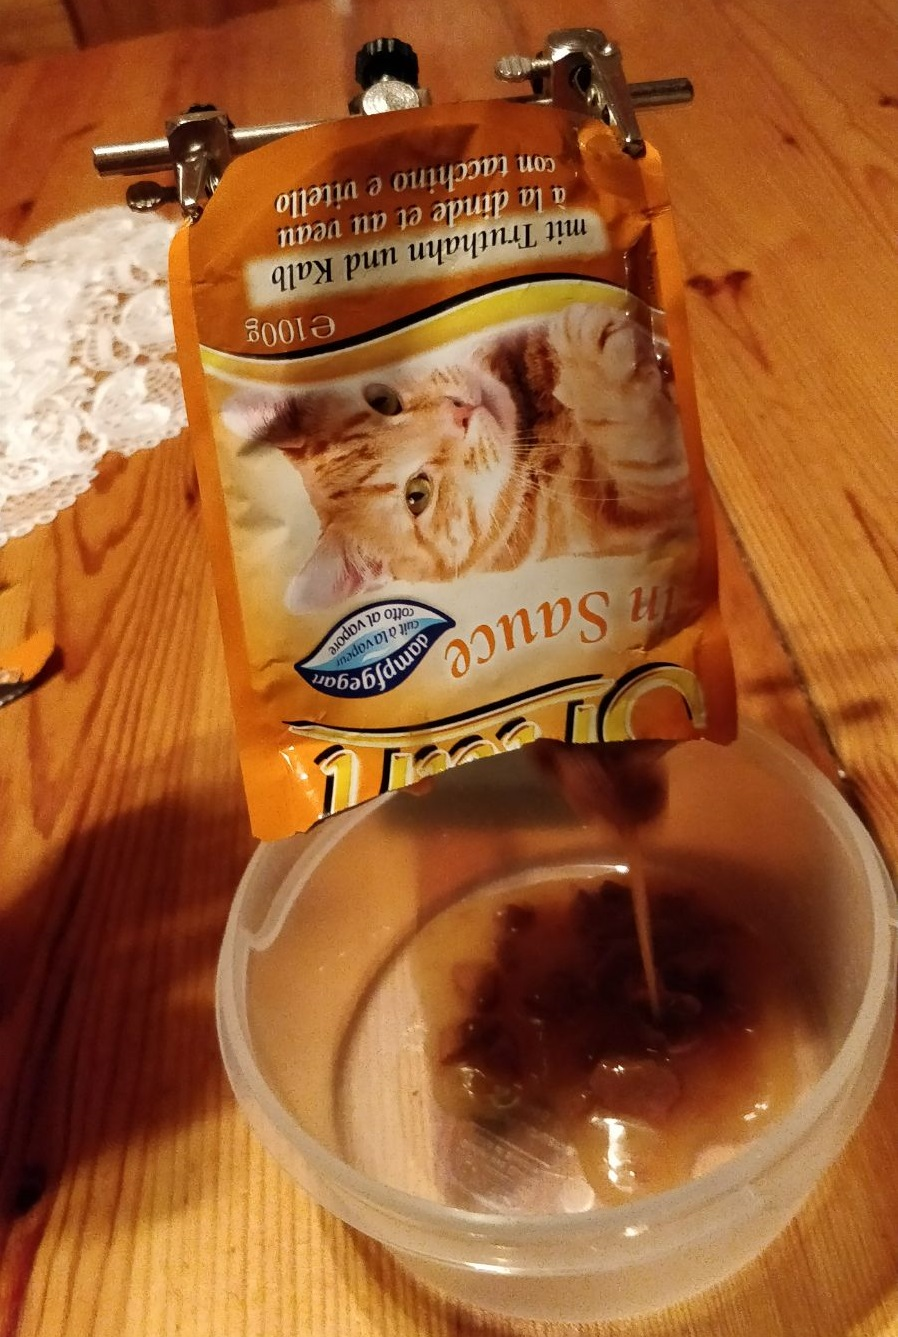
\includegraphics[width=\linewidth]{Bilder/Fuetterungsexperiment/Fuetterungs_Mitte}
      \caption{Entleerung nach 5min}
      \label{Fütterungs Mitte}
   \end{minipage}
   \hspace{.3\linewidth}% Abstand zwischen Bilder
   \begin{minipage}[hbt]{.33 \linewidth} % [b] => Ausrichtung an \caption
     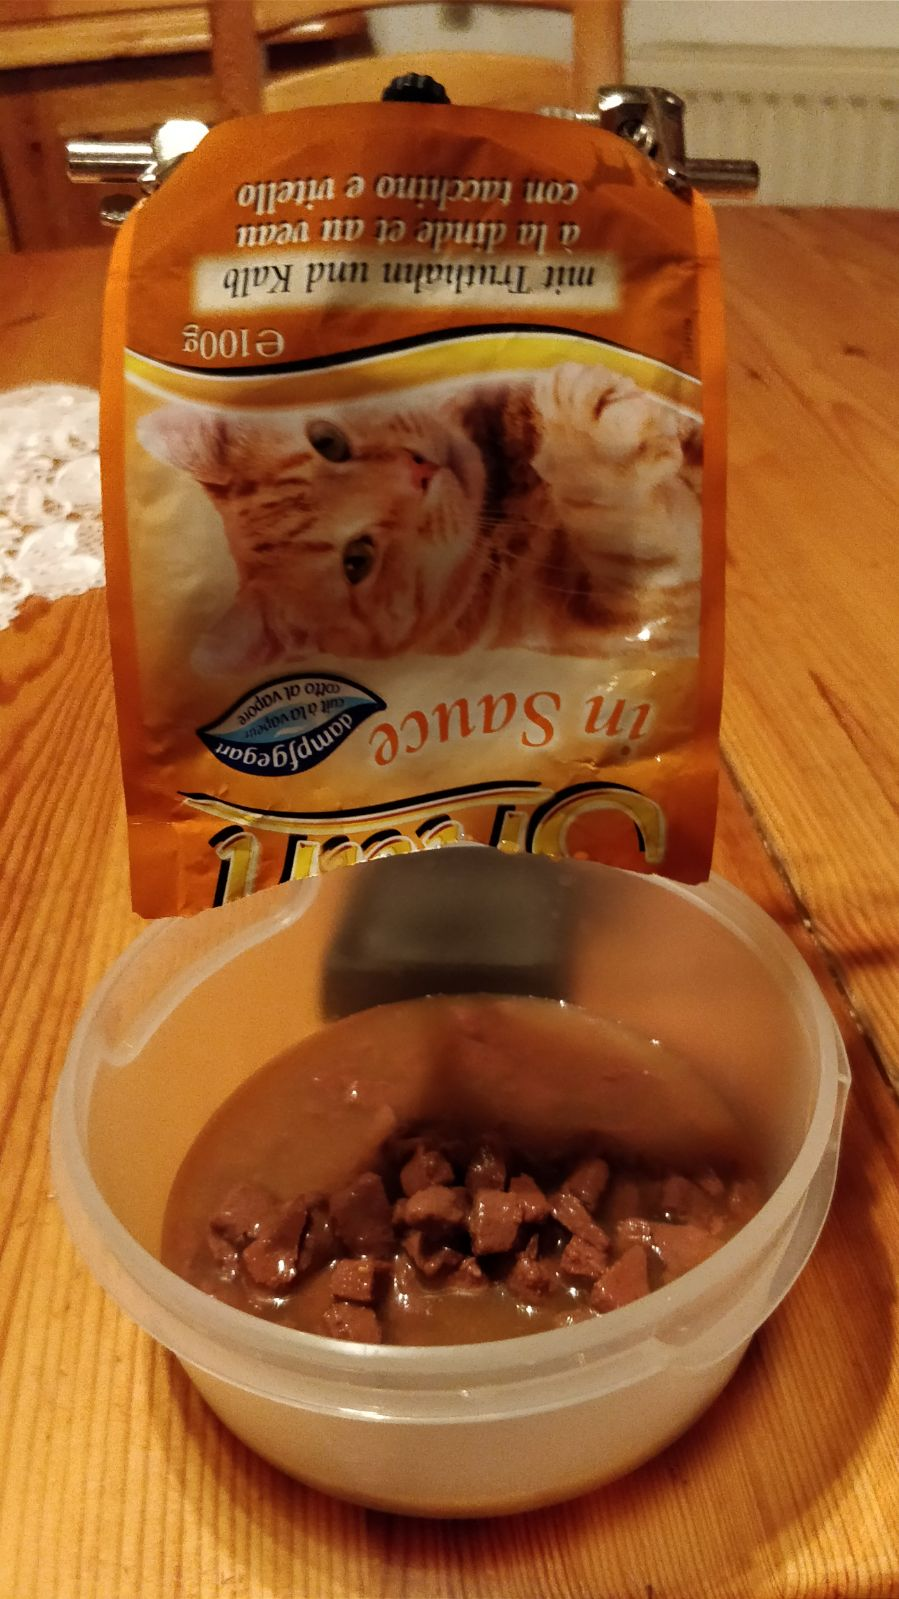
\includegraphics[width=\linewidth]{Bilder/Fuetterungsexperiment/Fuetterungs_Ende}  
      \caption{Entleerung nach 10min}
     \label{Fütterungs_Ende}
   \end{minipage}
\end{figure}
\newpage
\subsubsection{Schlussfolgerung des Fütterungsexperimentes}

Durch die Beobachtung lässt sich durch das Experiment folgende Schlussfolgerungen treffen: 
\begin{itemize}
\item Durch die leicht Gelee-artige aber eher dünnflüssige Konsistenz des Futters	rinnt es kontinuierlich innerhalb von 10 min aus der Packung.
\item Da der ganze Inhalt leicht gleitet, kann ohne Probleme durch eine Walze das restliche Futter ausgepresst werden.
\item Durch das Eigengewicht wird der Entleerungsprozess erleichtert.
\end{itemize} 

\subsection{Schneideversuch 1.Art der 1.Variante}

Schnitt anhand einer praxisnahen Anwendung dargestellt. Der Beutel wird mithilfe einer Papierschneidemaschine geschnitten. Siehe Abbildungen: \ref{Einlegen}, \ref{Anfangsschnitt}, \ref{Endschnitt}

\begin{figure}[H]
   \begin{minipage}[hbt]{.3\linewidth} % [b] => Ausrichtung an \caption
      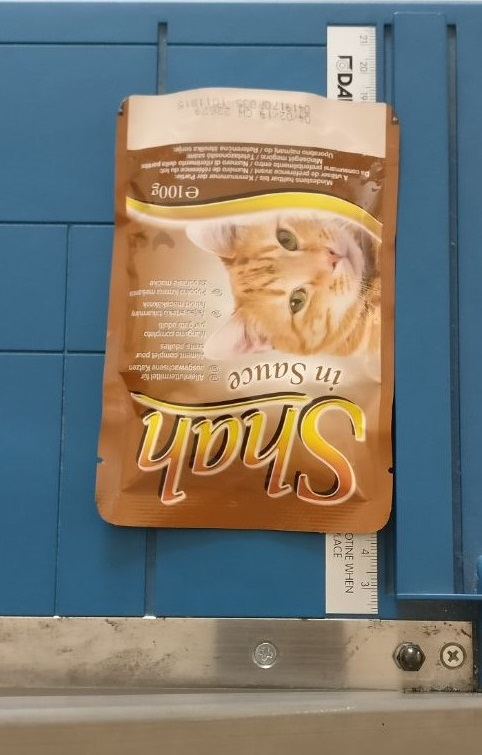
\includegraphics[width=\linewidth]{Bilder/Schneideversuch_1.Art/Einlegen}
      \caption{Einlegen}
      \label{Einlegen} 
   \end{minipage}
   \hspace{.2\linewidth}% Abstand zwischen Bilder
   \begin{minipage}[hbt]{.5\linewidth} % [b] => Ausrichtung an \caption
      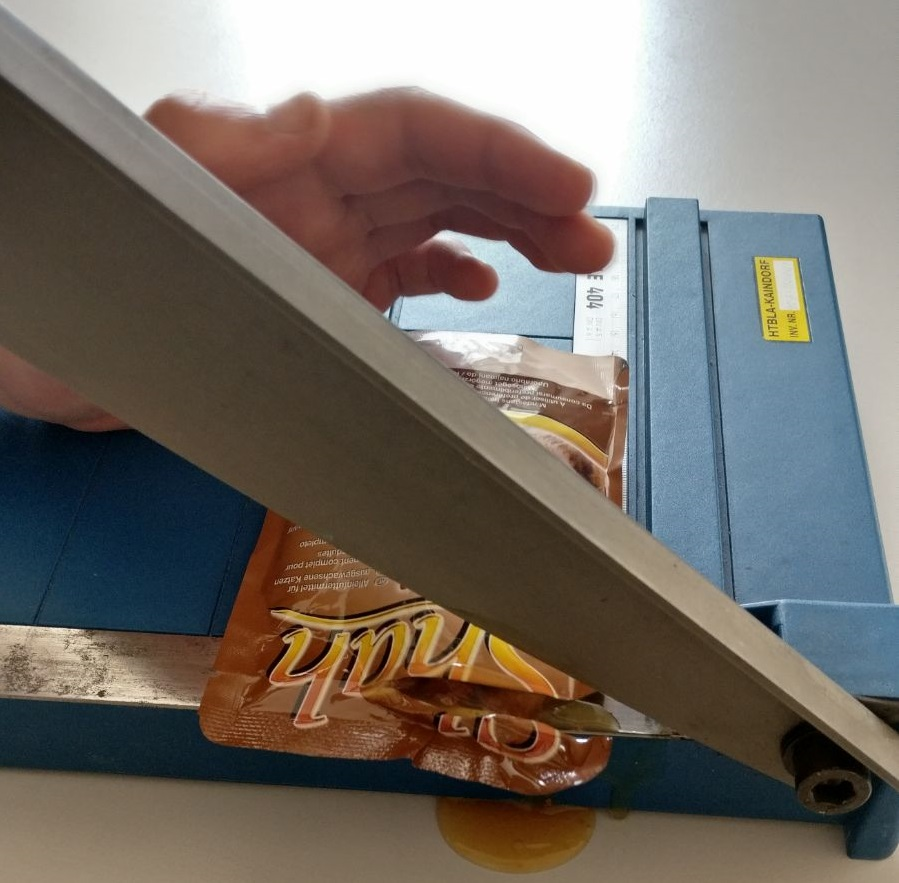
\includegraphics[width=\linewidth]{Bilder/Schneideversuch_1.Art/Anfangsschnitt}
      \caption{Anfangsschnitt}
      \label{Anfangsschnitt} 
   \end{minipage}
\end{figure}

\begin{figure}[H]
\begin{center}
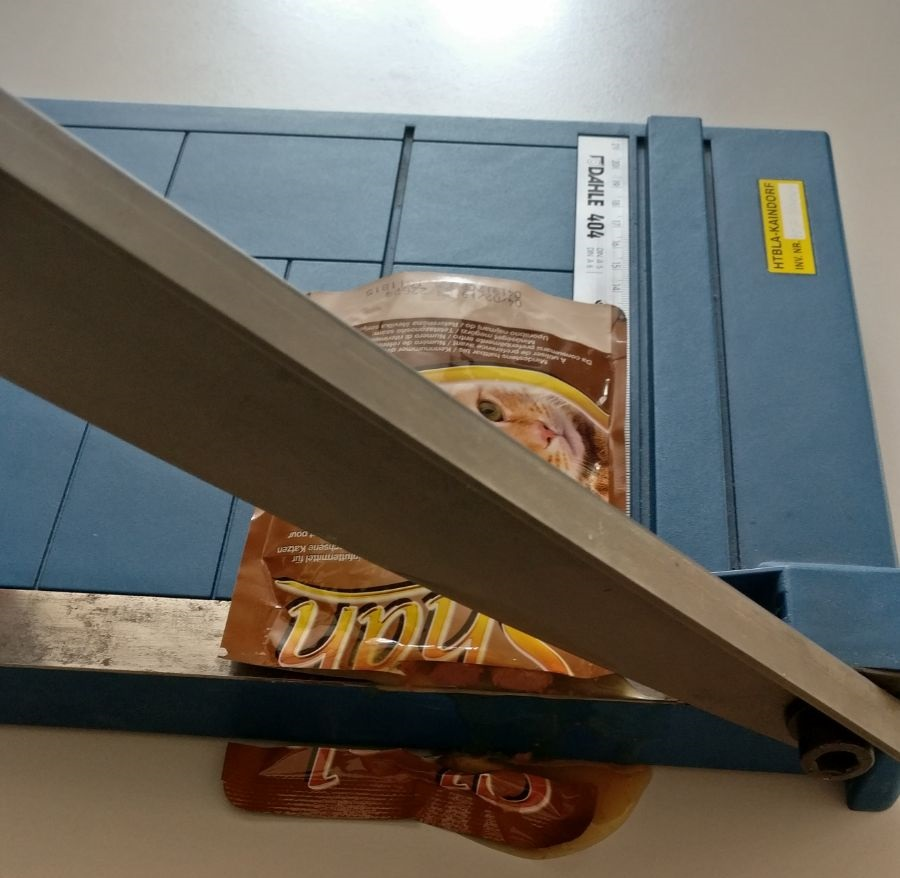
\includegraphics[width=7cm]{Bilder/Schneideversuch_1.Art/Endschnitt}
\caption{Endschnitt}
\label{Endschnitt} 
\end{center}
\end{figure}
\subsubsection{Schlussfolgerung des Schneideversuchs 1.Art der 1.Variante }

Diese ist von den beiden Schneidevarianten die bevorzugte und wurde durch  Abwiegen der pro und kontra ausgewählt.

In den folgenden Punkten sind die Ergebnisse von der ersten Variante aufgelistet:

\begin{itemize}
\item Durch den hohen Anpressdruck der Schneide an die Schneidplatte ließ sich die Packung vollständig öffnen.
\item Es gelang beim 1.Versuch mit nur einem durchgehenden Schnitt.
\item Die lange Klinge machte auch keine Probleme. Die Packung gelangte nicht zwischen die Schneidfläche und Klingen wurden nich auseinander gedrückt.
\item Die vom Futterhersteller vorgegebene Einkerbung kann mit realtiv wenig Kraft eine Rissfortpflanzung hervorgerufen werden(genauere Beschreibung unter Variante 1, Führen zur Schneidplatte).
\item Ein exaktes Positionieren und Schneiden war möglich.
\end{itemize} 
\newpage
\subsection{Schneideversuch 2.Art der 1.Variante}
\label{Schneideversuch_2}
Mit einem Metallwerkzeug mit wellenschliffartiger Kante wird der Futterbeutel entlang der Oberseite aufgeschnitten. Um die Packung vollständig geöffnet zu haben, mussten mehrere Schnitte verwendet werden. Siehe Abbildung: \ref{Schneidemittel}\\
In Abbildung: \ref{Nach 3 Schnitten} erkennt man wie offen die Packung nach 3 Schnitten ist.\\
In Abbildung: \ref{Nach 6 Schnitten} erkennt man wie offen die Packung nach 6 Schnitten ist.\\
In Abbildung: \ref{Nach 9 Schnitten} wurde die Packung nach 9 Schnitten vollständig geöffnet.

\begin{figure}[H]
   \begin{minipage}[hbt]{.3\linewidth} % [b] => Ausrichtung an \caption
      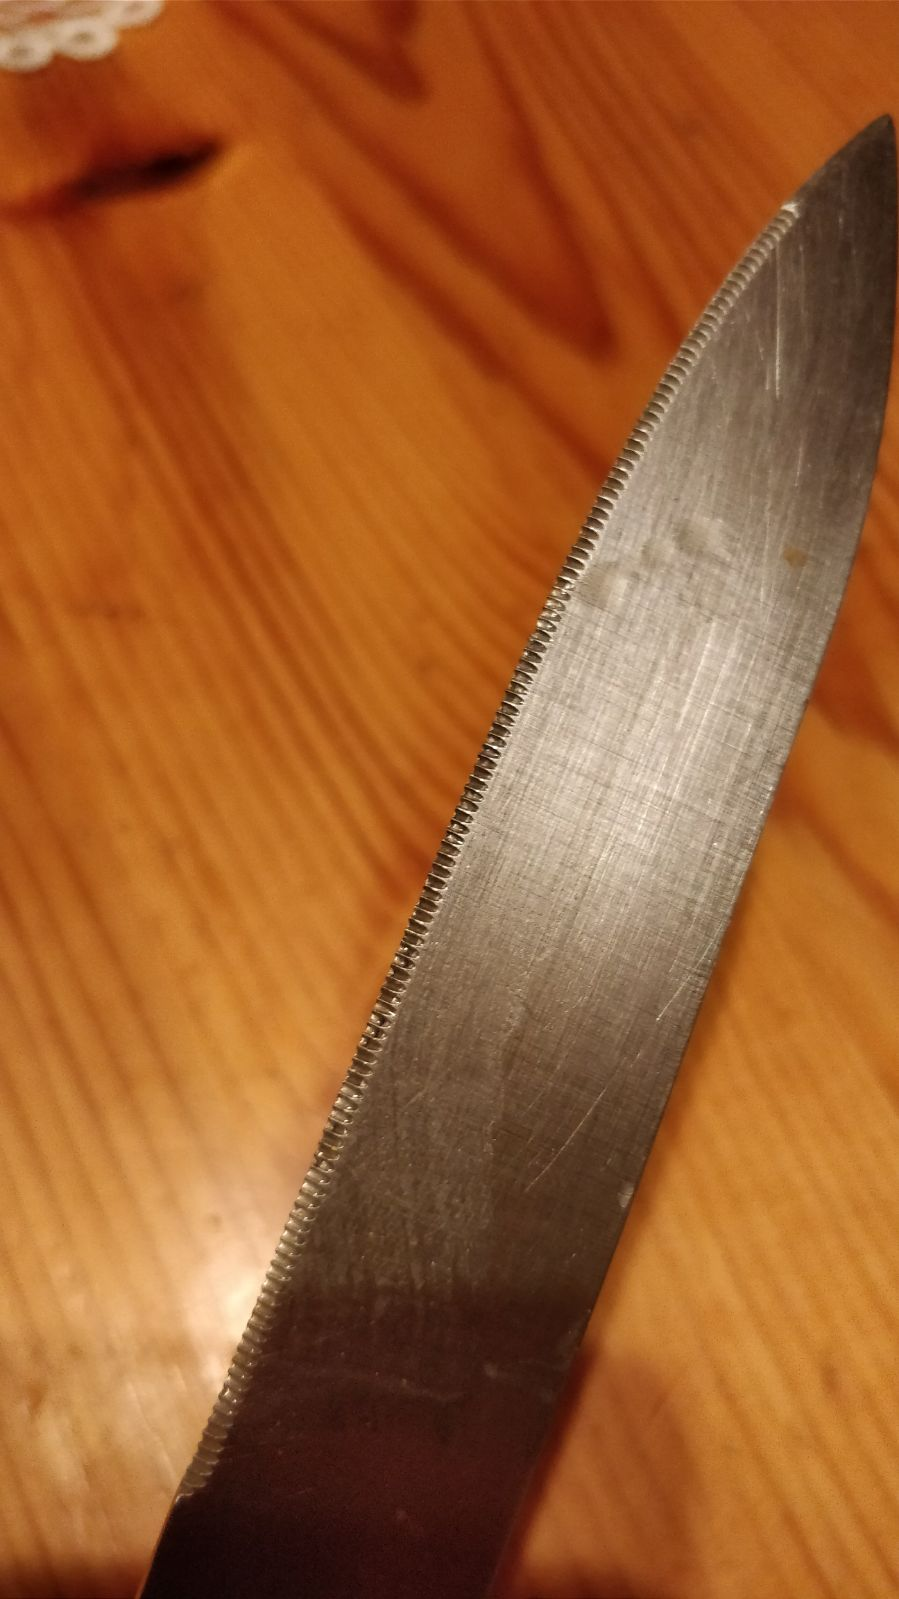
\includegraphics[width=\linewidth]{Bilder/Schneideversuch_2.Art/Schneidemittel}
      \caption{Schneidemittel}
      \label{Schneidemittel} 
   \end{minipage}
   \hspace{.4\linewidth}% Abstand zwischen Bilder
   \begin{minipage}[hbt]{.3\linewidth} % [b] => Ausrichtung an \caption
      
\includegraphics[width=\linewidth]{Bilder/Schneideversuch_2.Art/Anfangsschnitt}
      \caption{Anfangsschnitt 2.Art}
      \label{Nach 3 Schnitten}
   \end{minipage}
\end{figure}


\begin{figure}[H]
   \begin{minipage}[hbt]{.4\linewidth} % [b] => Ausrichtung an \caption
      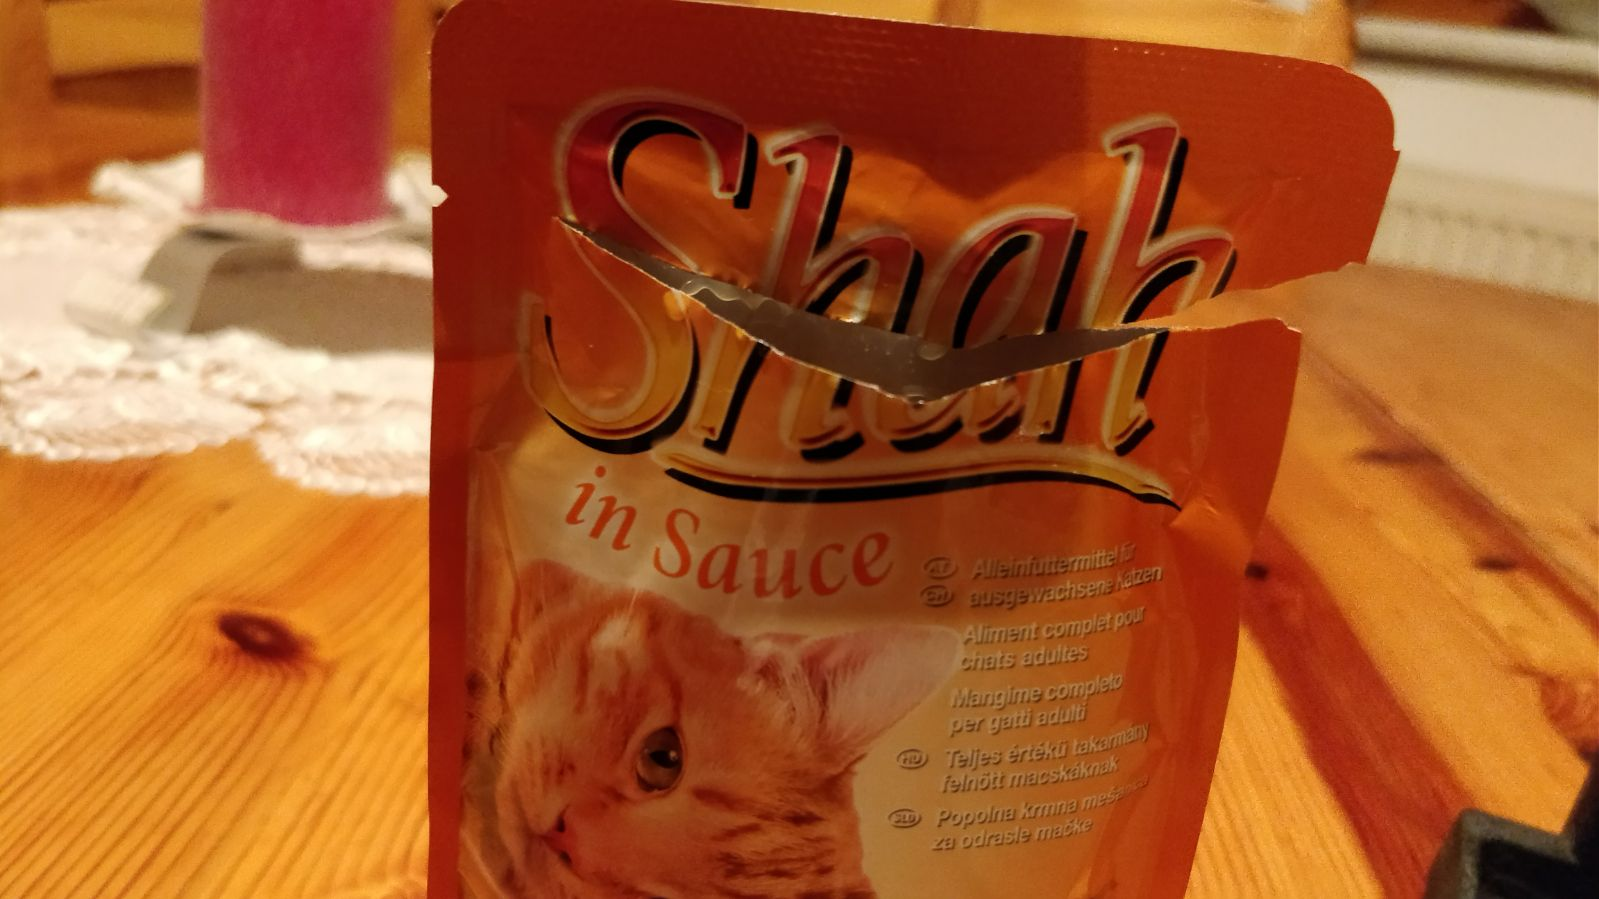
\includegraphics[width=\linewidth]{Bilder/Schneideversuch_2.Art/Mittelschnitt}
      \caption{Mittelschnitt 2.Art}
      \label{Nach 6 Schnitten}
   \end{minipage}
   \hspace{.2\linewidth}% Abstand zwischen Bilder
   \begin{minipage}[hbt]{.4\linewidth} % [b] => Ausrichtung an \caption
      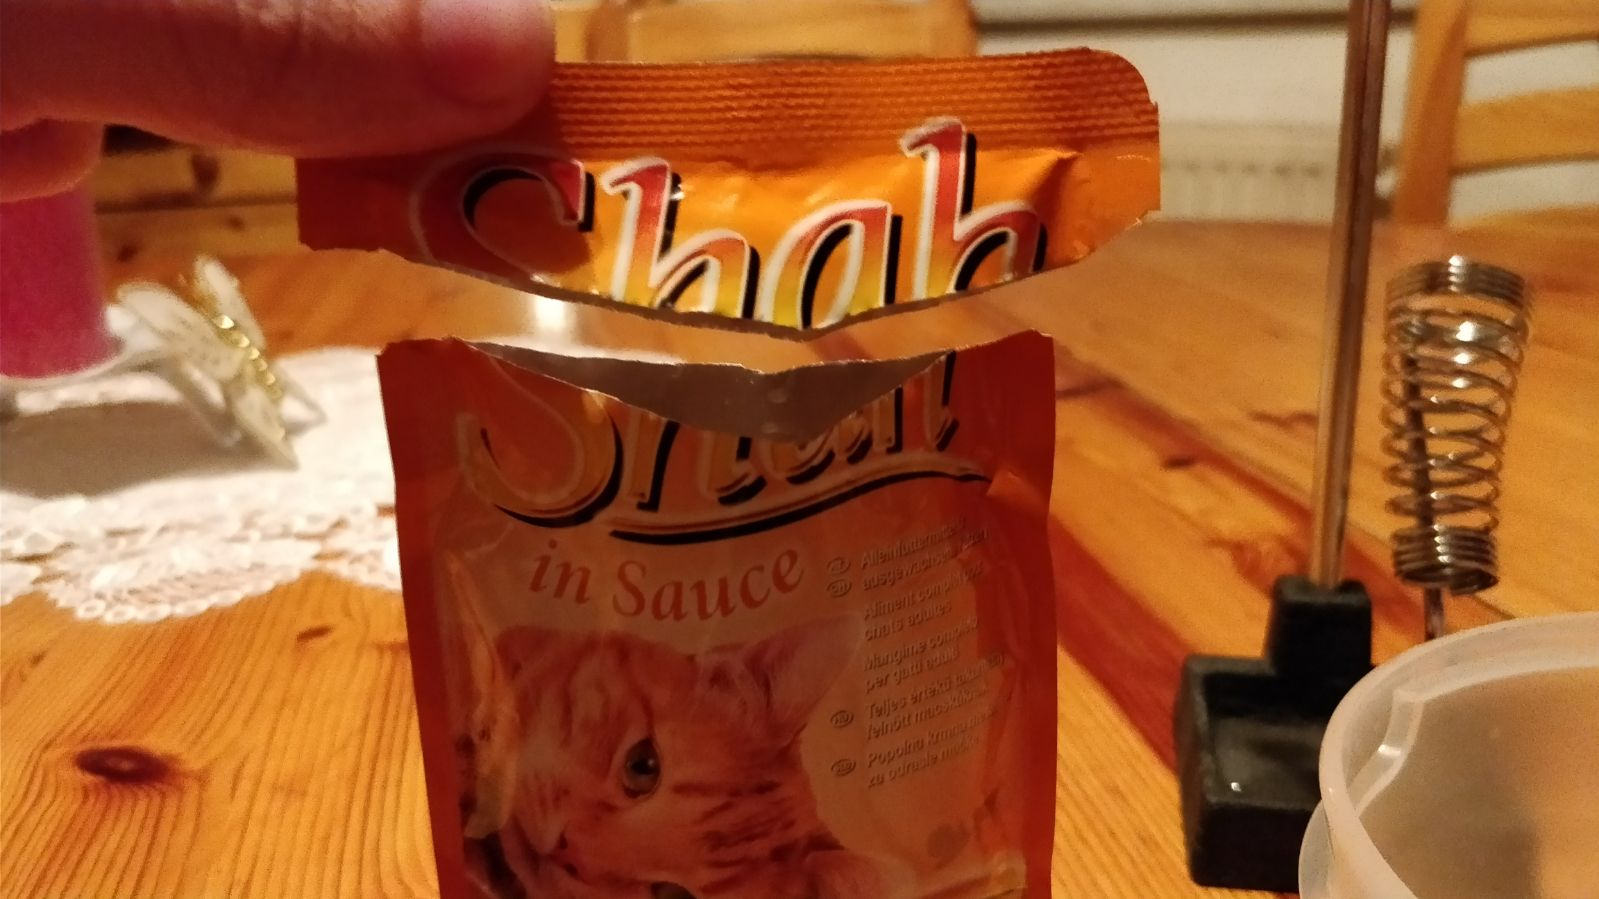
\includegraphics[width=\linewidth]{Bilder/Schneideversuch_2.Art/Endschnitt}
      \caption{Endschnitt 2.Art}
      \label{Nach 9 Schnitten}
   \end{minipage}
\end{figure}

\subsubsection{Schlussfolgerung des Schneideversuchs 2.Art der 1.Variante }

In den folgenden Punkten werden die Ergebnisse und auch Alternativen der zweiten Variante aufgelistet:

\begin{itemize}
\item Falls die Packung nicht genau eingespannt ist, kann durch die zackige Schneide kein guter Schnitt vollbracht werden, da die Klinge nicht schneidet sondern reißt.
\item Wenn der Schneidemechanismus auf diese Weise gelöst werden würde, müsste man das Messer durch ein Sägezahnrad ersetzen das mit eine Elektromotor angetrieben wird.
\item Es entsteht durch das Reißen der Verpackung, hervorgerufen durch die gezackte Klinge, kein gerader Schnitt.
\end{itemize}


\subsection{Dichtheitsexperiment der Hebelklemme}

\begin{wrapfigure}{r}{0.5\textwidth}
\vspace{-10pt}
  \begin{center}
    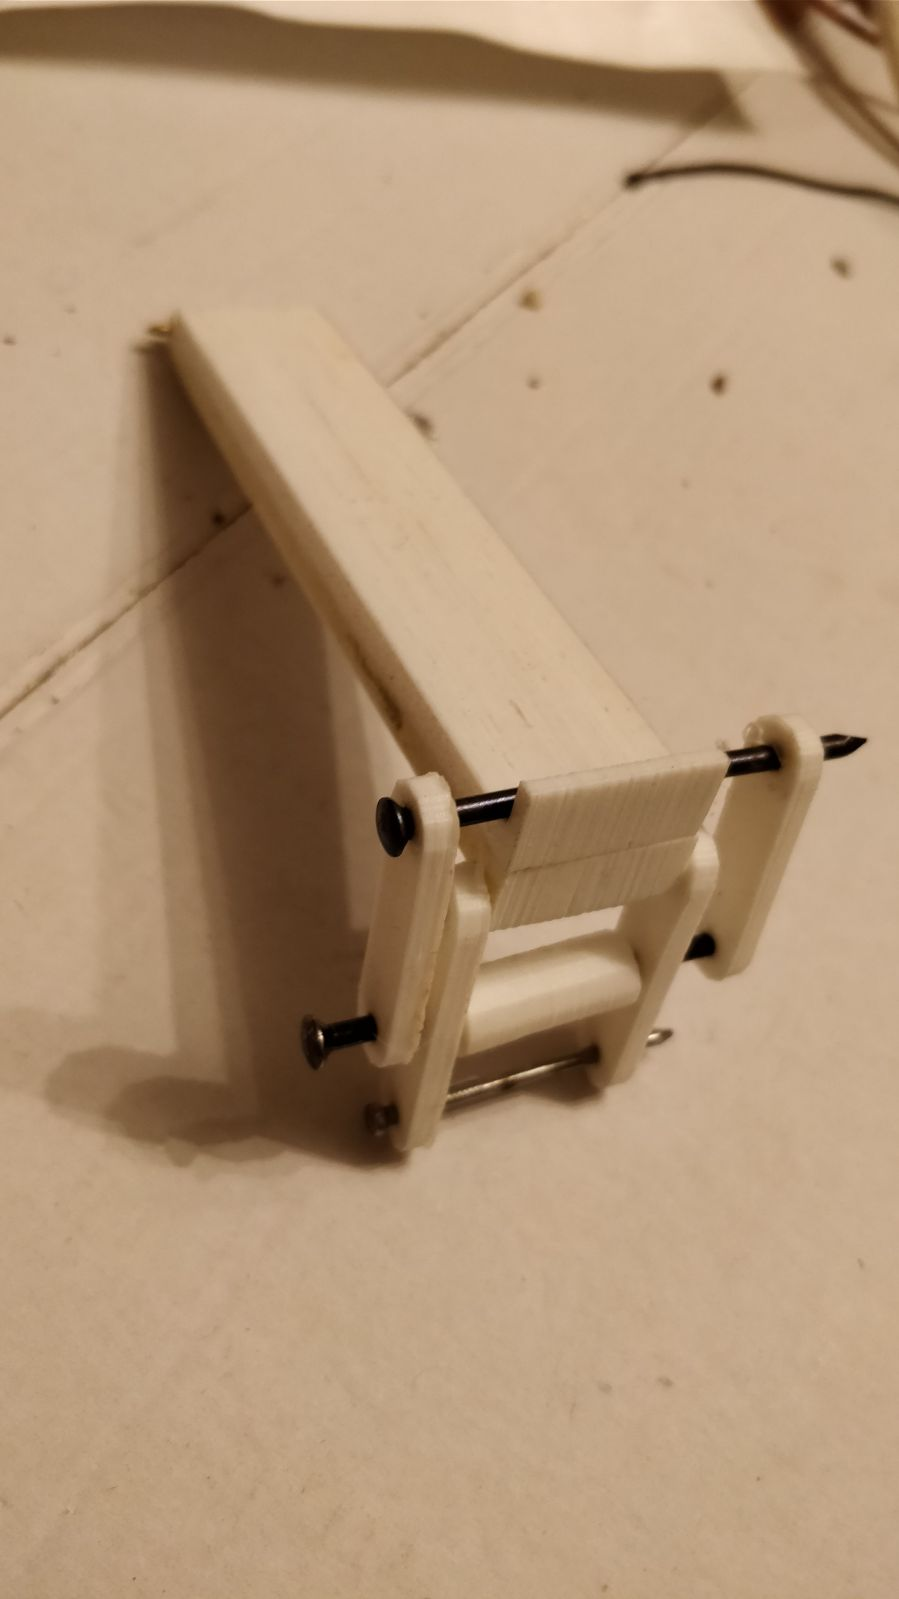
\includegraphics[width=0.22\textwidth]{Bilder/Dichtheitsexperiment/Klemme}
  \end{center}
  \caption{3D-Klemme}
  \label{3D-Klemme}
  \vspace{-20pt}
\end{wrapfigure}

Die für unsere Maschine entscheidende Klemme wurde 3D gedruckt. Die damit verschlossene Verpackung wurde 5 Tage getestet. Von der Klemme wurde nur die Umrandung der einzelnen Teile gedruckt das heißt die Teile sind in der Mitte hohl und dehnbarer bzw. biegsamer als massive Teile für die Klemme. Im Bild: \ref{3D-Klemme} erkennt man den ersten Prototypen der Klemme. Die gedruckten Teile werden mit 1,5mm dicke Nägel verbunden. Die Klemme wird im richtigen Modell mit Metall gebaut und die Nägel werden durch passende Stifte ersetzt.\\\\ 
Die tatsächliche Klemme sollten dann statt aus Kunstoff z.B. aus Aluminium hergestellt werden. Durch den höheren Elastizitätsmodul erhöht sich die Wahrscheinlichkeit der Dichtheit noch weiter.

Die Aufgabe der Klemme war, diese fünf Tage senkrecht aufzuhängen und die Klemme auf stärken und schwächen zu Prüfen.\\

Tag 1: Die Klemme wurde samt der Packung senkrecht aufgehängt und an den von Futterhersteller vorgegeben Schneidepunkt aufgeschnitten. Siehe Abbildung: \ref{Klemme_Tag_1}. Der erste Eindruck war, dass die Klemme dicht hält ohne menschliche Einflüsse. Sobald die Klemme wenig gepresst wurde ran die Flüssigkeit aus der Klemme, weil diese nicht massiv bzw. stabil genug ist. Die beiden längeren Flächen die über die Packung gelegt werden bogen sich durch die menschliche Einwirkung (Erhöhung der Druckes in der Packung)auseinander. Dennoch war die Klemme, wenn sie sich in Ruhelage befand dicht.

\begin{figure}[H]
   \begin{minipage}[hbt]{.5\linewidth} % [b] => Ausrichtung an \caption
      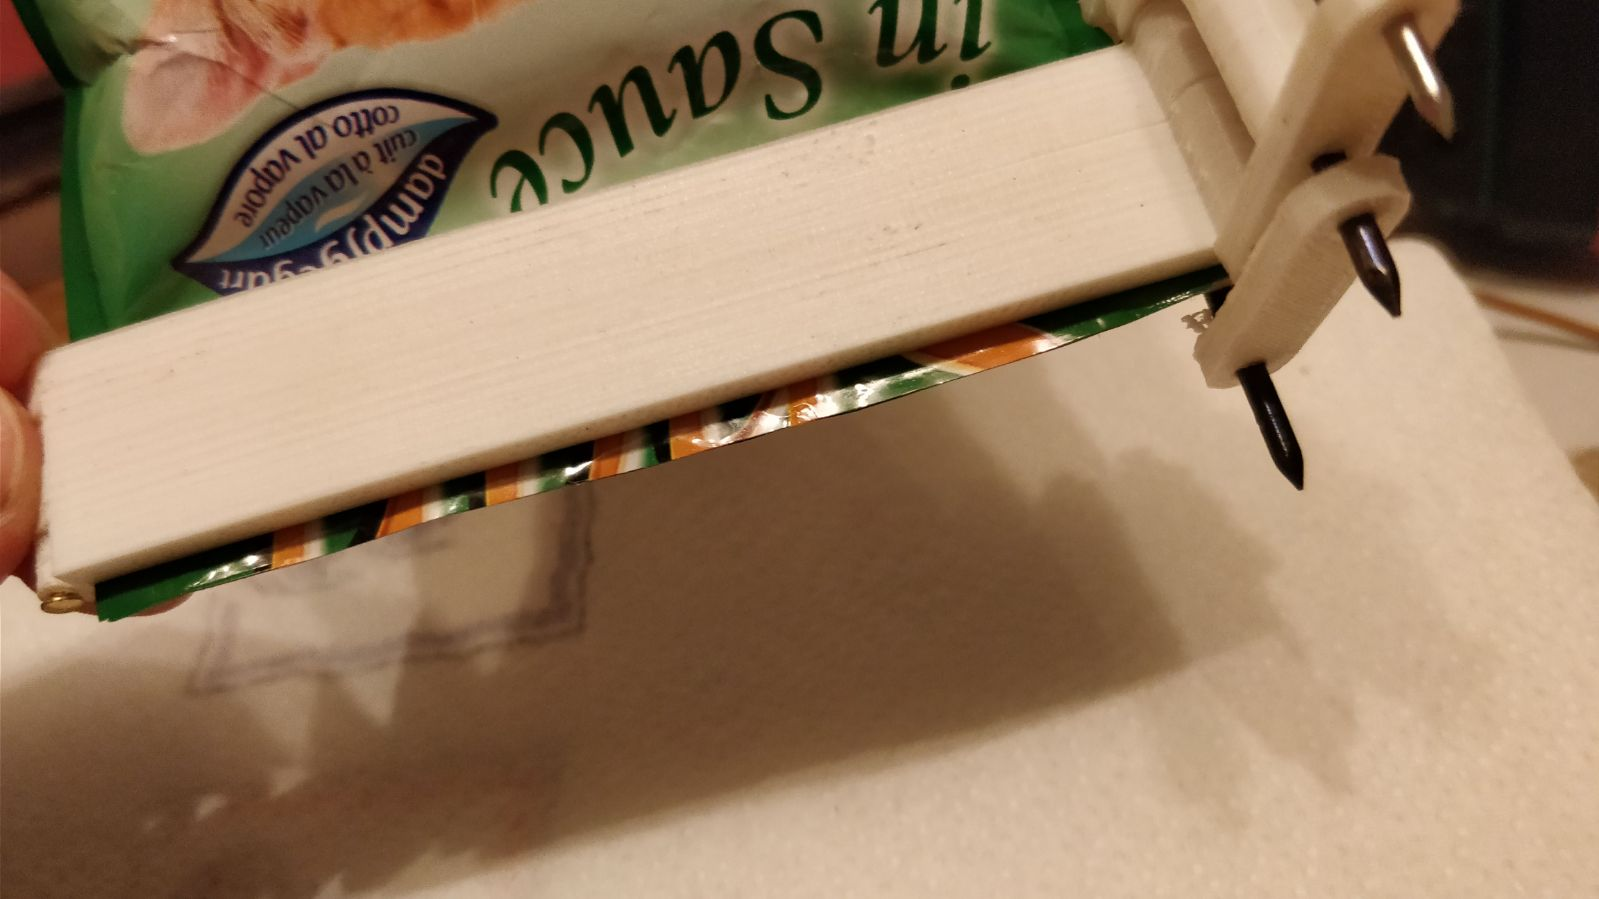
\includegraphics[width=\linewidth]{Bilder/Dichtheitsexperiment/Probe}
      \caption{Klemmen Probe}
      \label{Klemmen_Probe} 
   \end{minipage}
   \hspace{.2\linewidth}% Abstand zwischen Bilder
   \begin{minipage}[hbt]{.3\linewidth} % [b] => Ausrichtung an \caption
      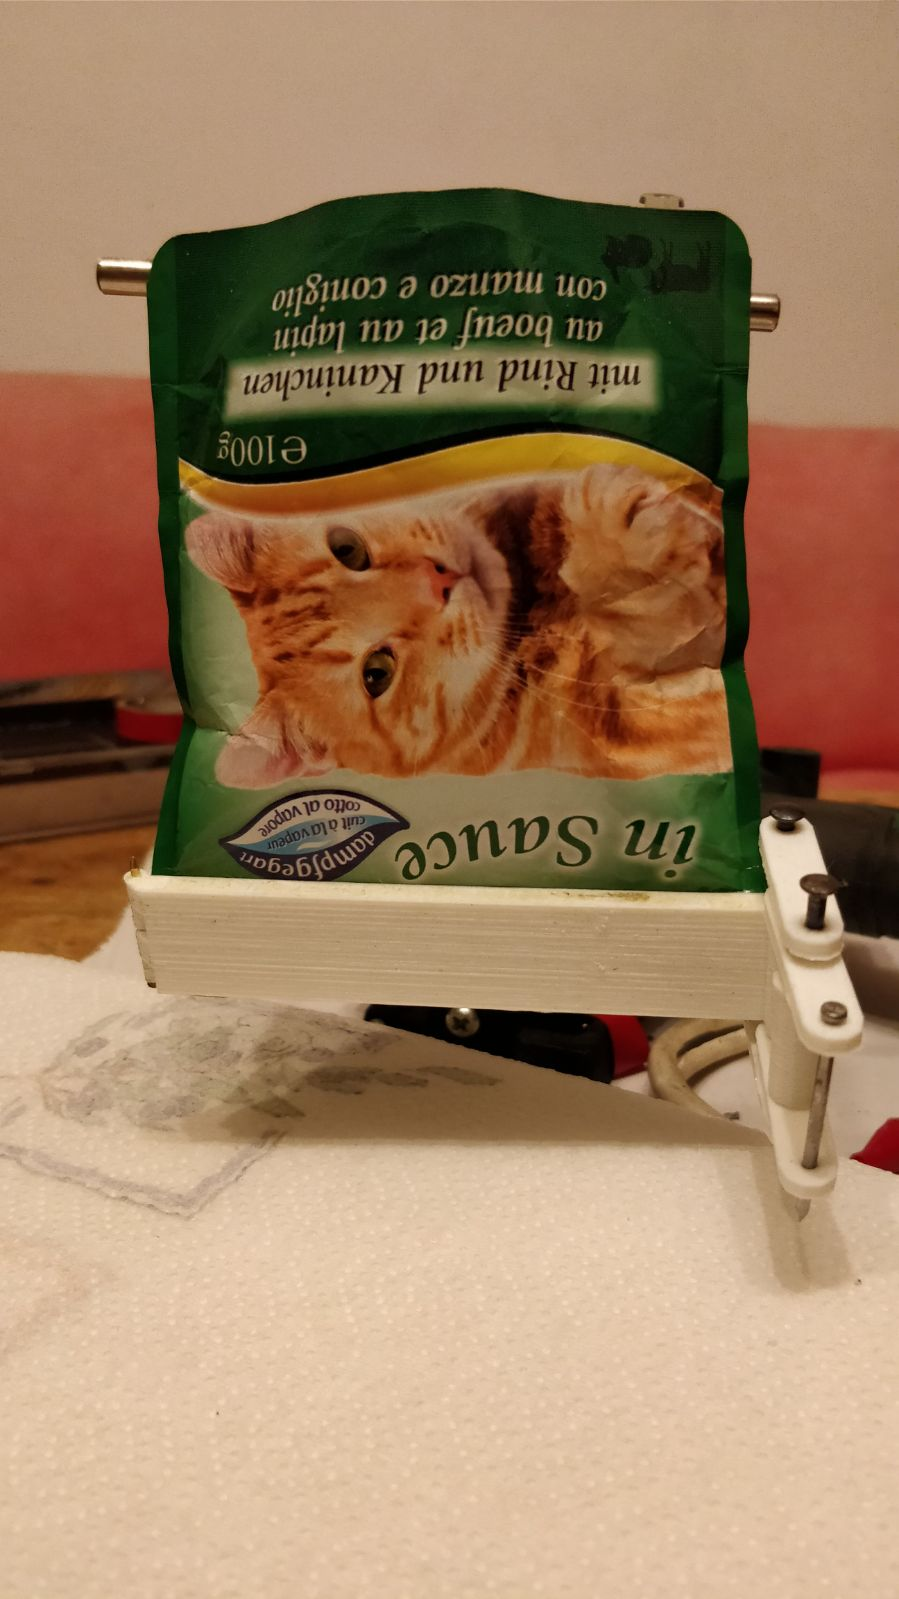
\includegraphics[width=\linewidth]{Bilder/Dichtheitsexperiment/Tag_1}
      \caption{Klemme Tag 1}
      \label{Klemme_Tag_1}
   \end{minipage}
\end{figure}

Tag 2: Zur Überprüfung ob die Packung dicht hält wurde eine weiße Unterlage darunter geschoben in diesem Fall ein Blatt-Küchenrolle. Auch hier sieht man durch einen bildlichen Beweis das unter der Packung nichts verschmutzt ist. Siehe Abbildung: \ref{Klemme_Tag_2}. \\

Tag 3: Das gleiche Resultat wie am Tag 1 und 2. Siehe Abbildung: \ref{Klemme_Tag_3}.

\begin{figure}[H]
   \begin{minipage}[hbt]{.3\linewidth} % [b] => Ausrichtung an \caption
      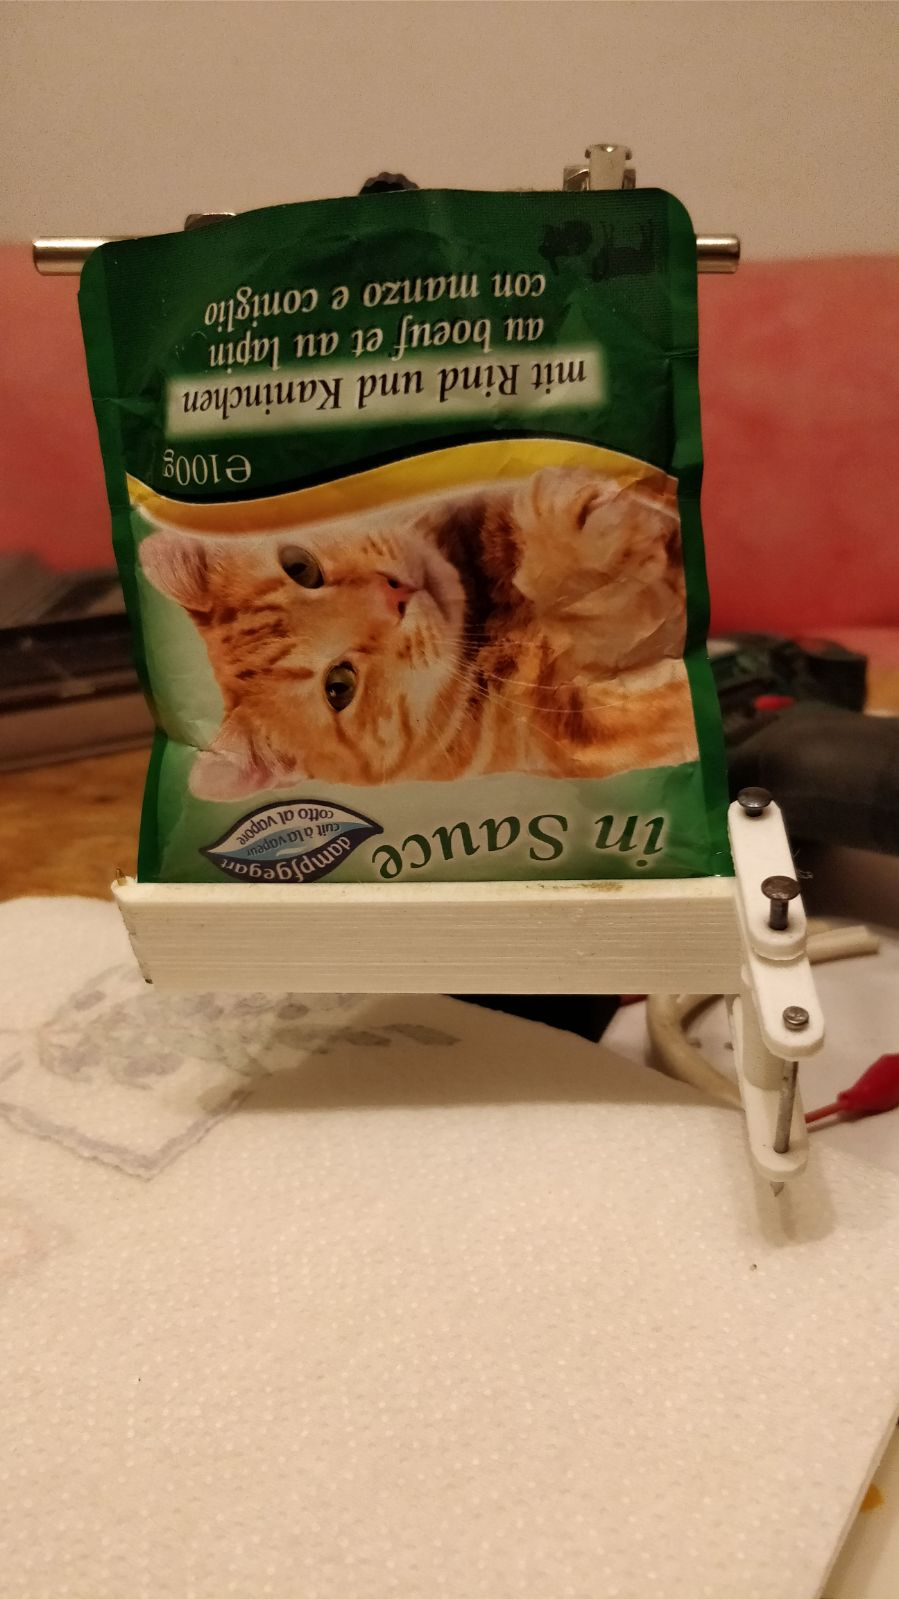
\includegraphics[width=\linewidth]{Bilder/Dichtheitsexperiment/Tag_2}
      \caption{Klemme Tag 2}
      \label{Klemme_Tag_2} 
   \end{minipage}
   \hspace{.3\linewidth}% Abstand zwischen Bilder
   \begin{minipage}[hbt]{.3\linewidth} % [b] => Ausrichtung an \caption
      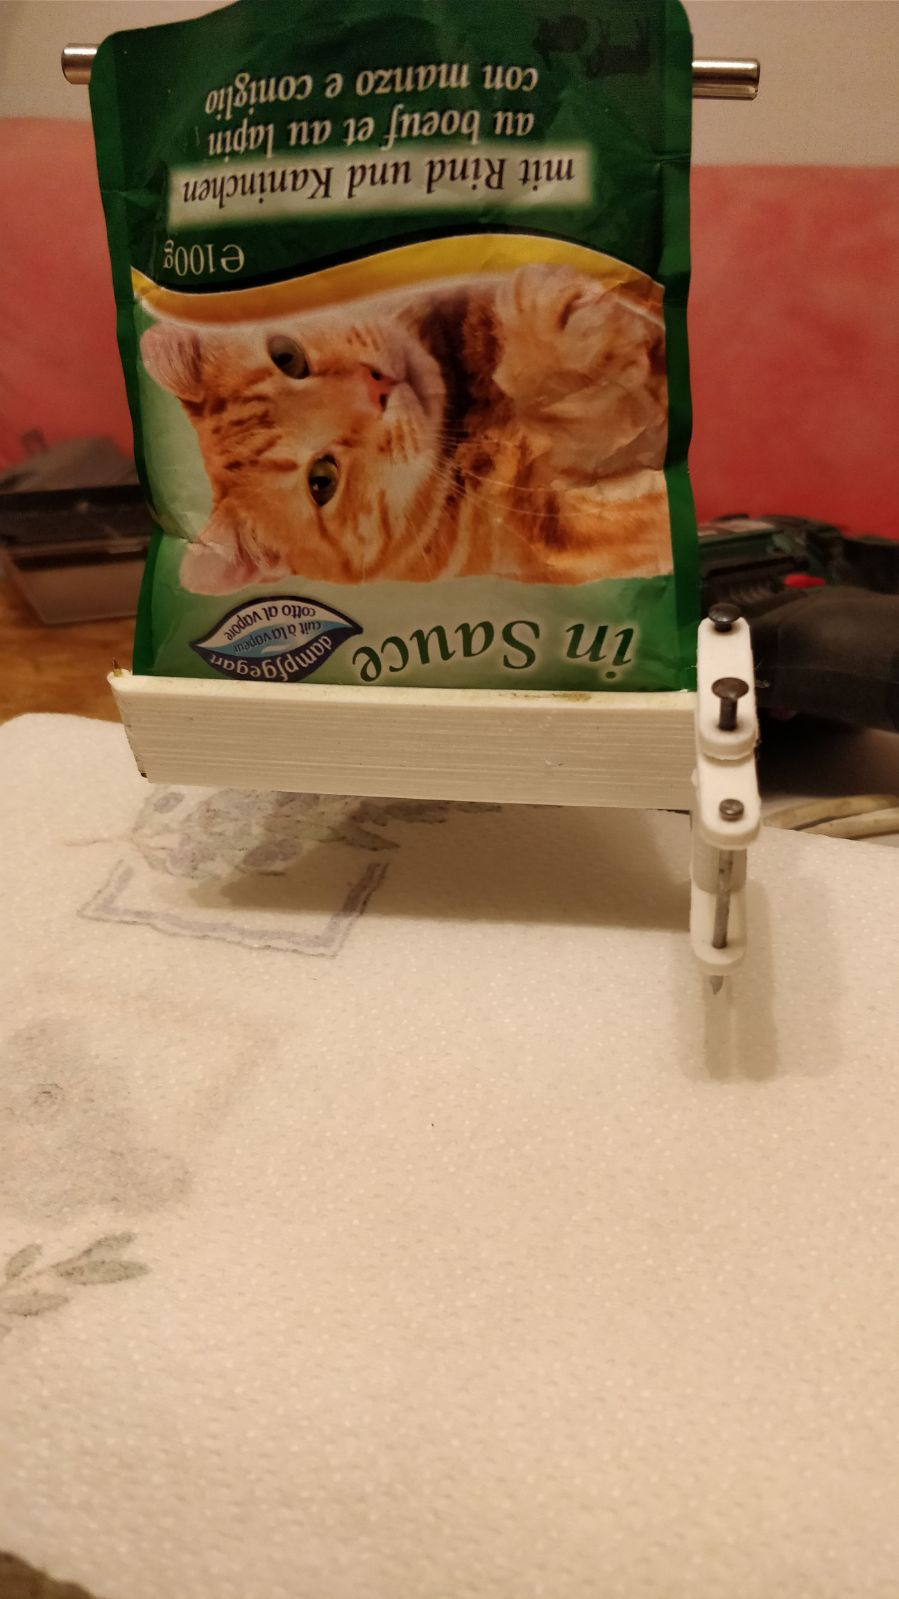
\includegraphics[width=\linewidth]{Bilder/Dichtheitsexperiment/Tag_3}
      \caption{Klemme Tag 3}
      \label{Klemme_Tag_3}
   \end{minipage}
\end{figure}

Tag 4: Wie am Bild \ref{Klemme_Tag_4} zu sehen war am vierten Tag auch keine Flüssigkeit am Tuch. Siehe Abbildung: \ref{Klemme_Tag_4}.\\ 

Tag 5: Der Beweiß ist vollbracht. Die ganzen fünf Tage die der Benutzer im Urlaub ist hält auch die in stabilere Klemme dicht. Siehe Abbildung: \ref{Klemme_Tag_5}.

\begin{figure}[H]
   \begin{minipage}[hbt]{.3\linewidth} % [b] => Ausrichtung an \caption
      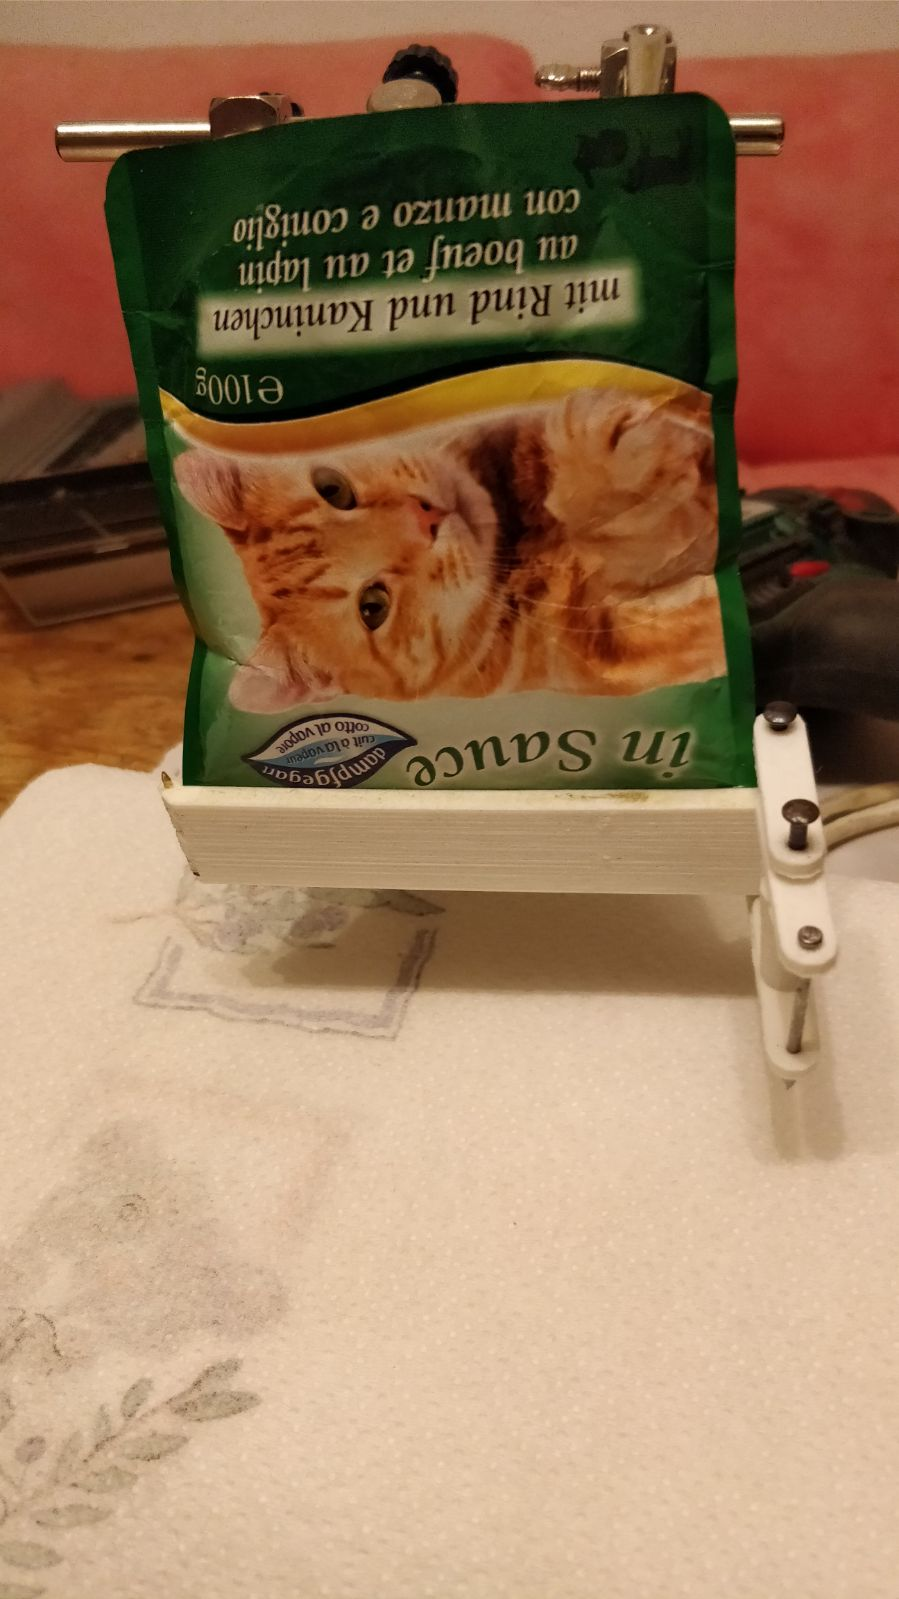
\includegraphics[width=\linewidth]{Bilder/Dichtheitsexperiment/Tag_4}
      \caption{Klemme Tag 4}
      \label{Klemme_Tag_4} 
   \end{minipage}
   \hspace{.3\linewidth}% Abstand zwischen Bilder
   \begin{minipage}[hbt]{.3\linewidth} % [b] => Ausrichtung an \caption
      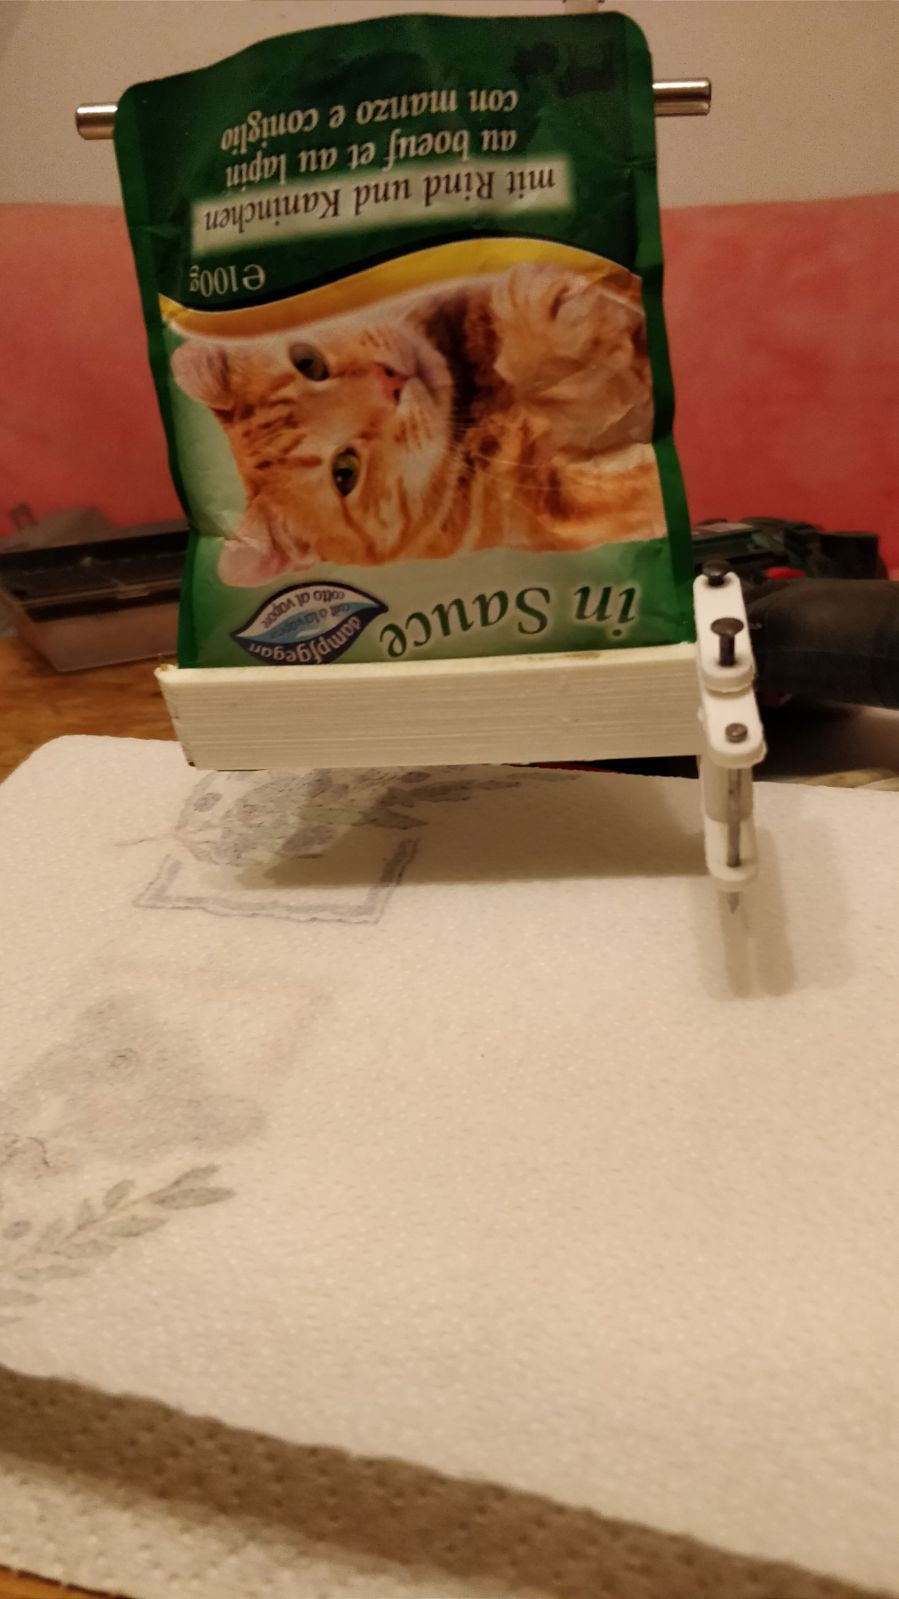
\includegraphics[width=\linewidth]{Bilder/Dichtheitsexperiment/Tag_5}
      \caption{Klemme Tag 5}
      \label{Klemme_Tag_5}
   \end{minipage}
\end{figure}

\subsection{Zustand der Futterpackung nach dem Urlaub}

Es wurde die Beschaffenheit und die Konsistenz des Futters nach fünf Tagen getestet. Dazu wurde eine Verpackung mit der Hebel-Klemme versehrt und hängend in einen Raum platziert. Um eine Sicherheit einzuplanen hing der Futterbeutel 3 Wochen. Nach Ablauf dieser Zeit sind wir diesen Schlussfolgerungen gekommen: 

\begin{itemize}
\item Aus der Futterpackung ist keine Flüssigkeit ausgetreten. Dies erkennt man daran, dass der Rand nicht verschmutzt bzw. verkrustet  und die weiße Unterfächer Fleckenfrei war. Siehe Abbildung: \ref{Fütterungsexperiment_Ende}.
\item Des Weiteren war das Futter weder von Schimmel befallen noch roch es schlecht. Siehe Abbildung: \ref{Futter_Ende_1}.
\item Zu guter Letzt die Geschmacksprobe. Dies wurde bewiesen indem die Katze die ganze Schüssel fraß. Siehe Abbildung: \ref{Ansicht_von_der_Futterschüssel}.

\end{itemize} 

\begin{figure}[H]
   \begin{minipage}[hbt]{.4\linewidth} % [b] => Ausrichtung an \caption
      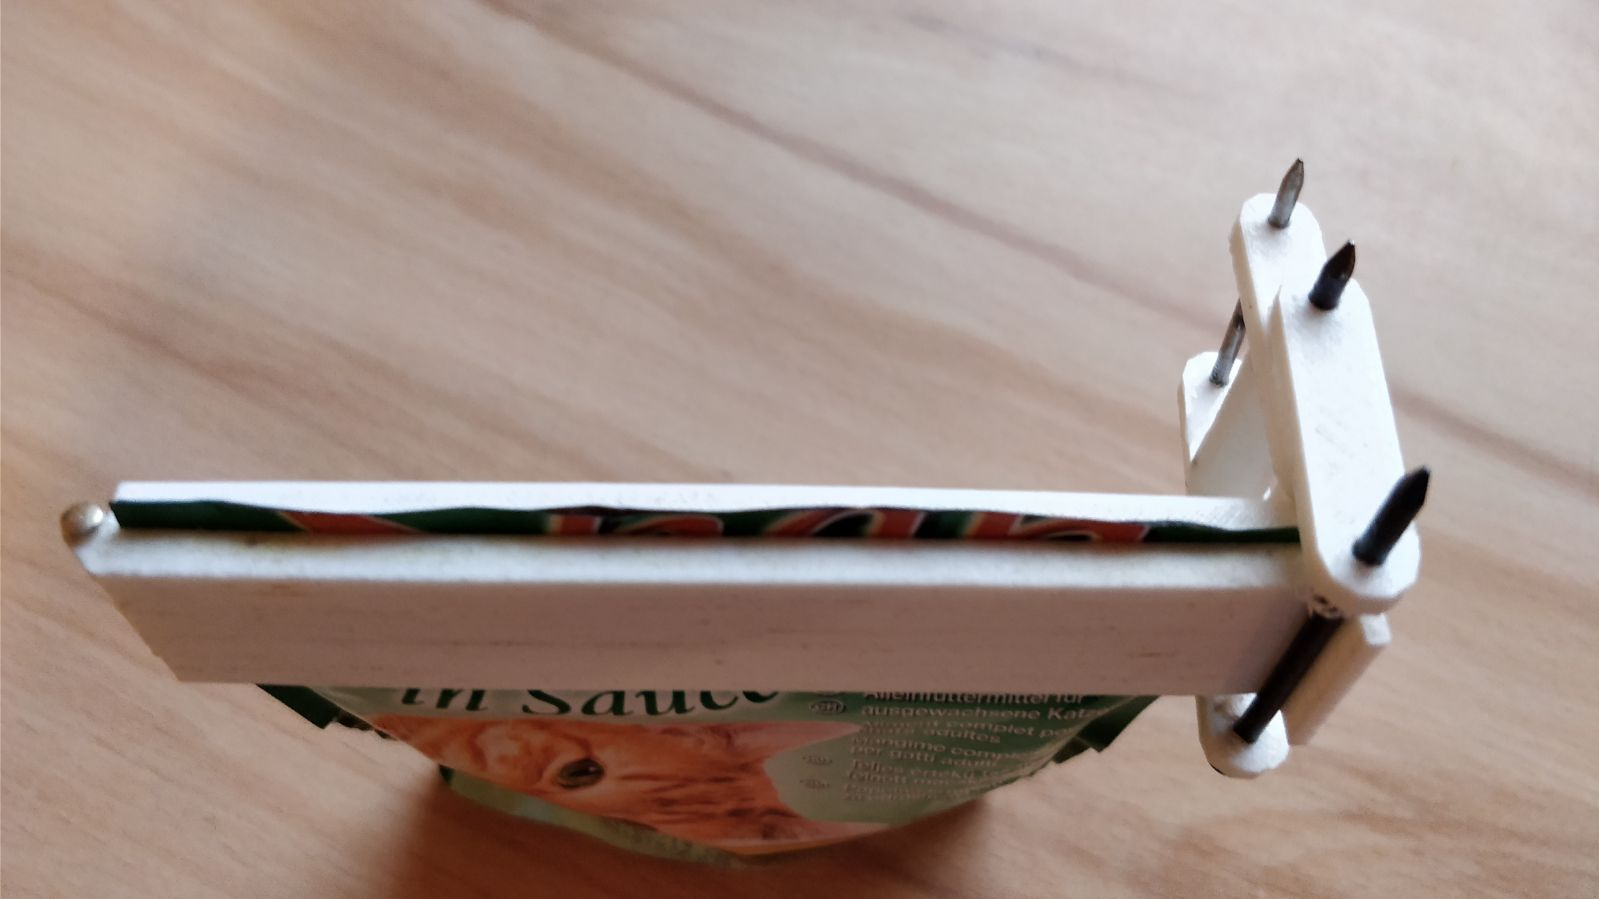
\includegraphics[width=\linewidth]{Bilder/Futterungsexperiment_Ende/Futter_Ende}
      \caption{Fütterungsexperiment Ende}
      \label{Fütterungsexperiment_Ende} 
   \end{minipage}
   \hspace{.2\linewidth}% Abstand zwischen Bilder
   \begin{minipage}[hbt]{.4\linewidth} % [b] => Ausrichtung an \caption
      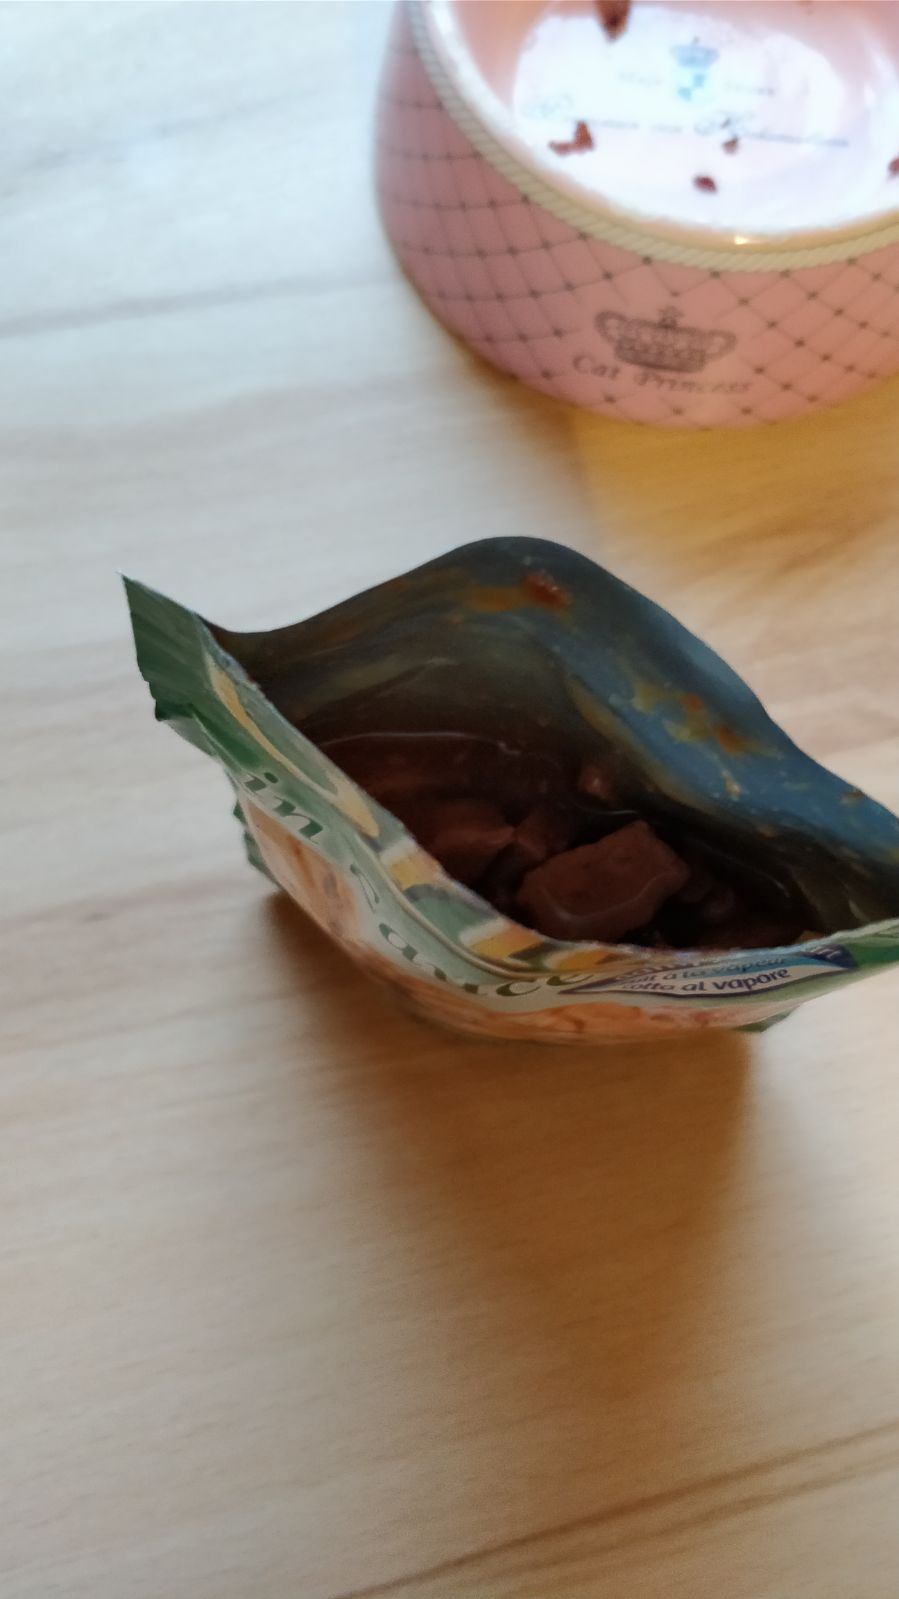
\includegraphics[width=\linewidth]{Bilder/Futterungsexperiment_Ende/Futter_Ende_1}
      \caption{Futterkonsistenz}
      \label{Futter_Ende_1}
   \end{minipage}
\end{figure}

\begin{figure}[H]
\begin{center}
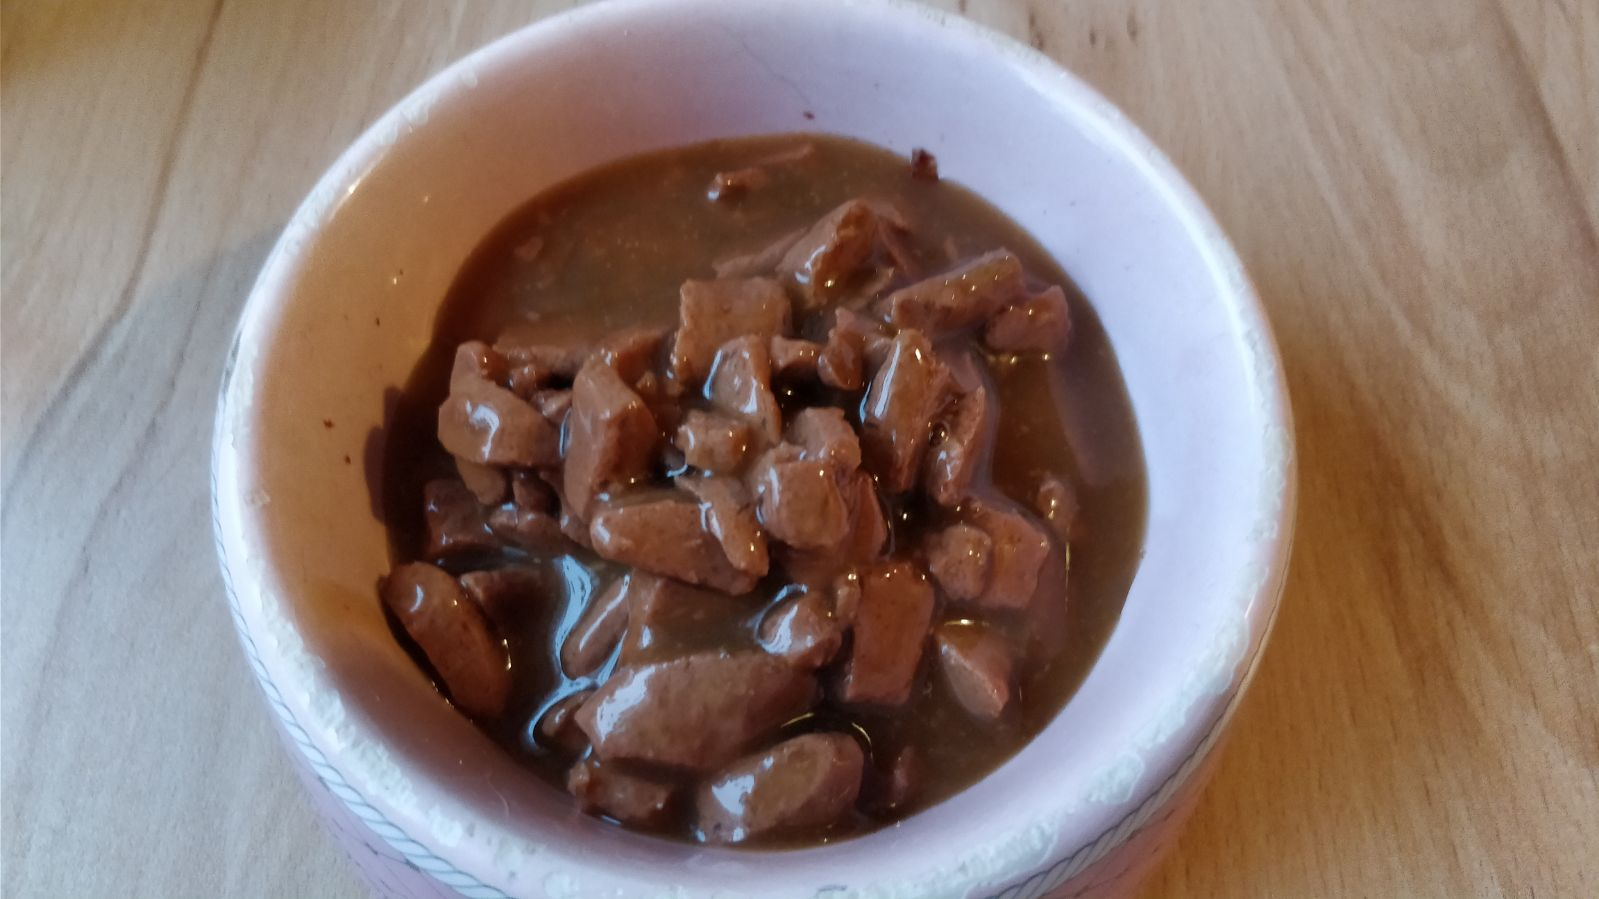
\includegraphics[width=8cm]{Bilder/Futterungsexperiment_Ende/Futter_Ende_2}
\caption{Futter in der Schüssel}
\label{Ansicht_von_der_Futterschüssel} 
\end{center}
\end{figure}


\section{Vergleich der Varianten}

In diesem Kapitel der Diplomarbeit werden sämtliche Ideen Schemenhaft gezeichnet und erklärt.
 
\subsection{Klemmen}

Es wurden verschiedene Varianten durchdacht, auf welche Wege die Packung luftdicht verschlossen werden kann. Dabei sind die folgenden Mechanismen entstanden.

\subsubsection{Einfache Klemme}

\begin{wrapfigure}{r}{0.5\textwidth}
\vspace{-20pt}
  \begin{center}
    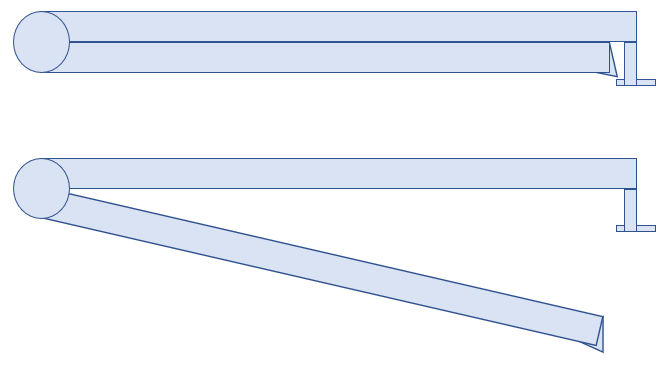
\includegraphics[width=0.32\textwidth]{Bilder/Powerpoint/Einfach_Klemme}
  \end{center}
  \caption{Einfache Klemme}
  \label{Einfache Klemme}
  \vspace{-10pt}
\end{wrapfigure}

Die einfache Klemme ist für gewöhnliche Verpackungen gut zu nutzen, jedoch ist sie für unsere Variante nicht zu gebrauchen, weil Kunststoff nicht so stabil wie Metall ist. Drückt die Kunststoffklemme die Packung an manchen Stellen zu wenig zusammen, kann Flüssigkeit austreten. Außerdem hält sie bei Zugbelastung schlechter als Metall. Siehe Abbildung: \ref{Einfache Klemme}

\subsubsection{Hebel-Klemme} 

\begin{wrapfigure}{r}{0.5\textwidth}
\vspace{-30pt}
  \begin{center}
    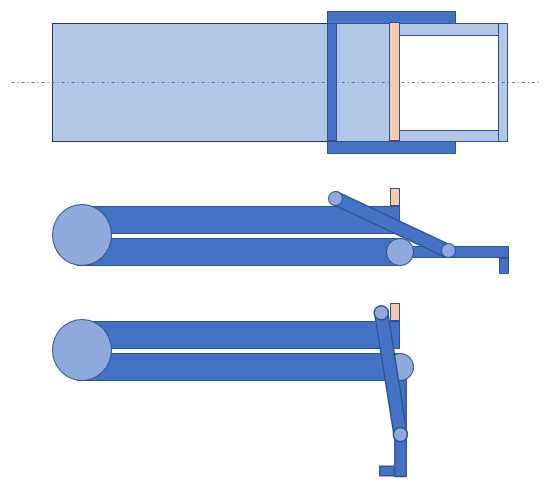
\includegraphics[width=0.32\textwidth]{Bilder/Powerpoint/Hebel_Klemme}
  \end{center}
  \caption{Hebel Klemme}
  \label{Hebel Klemme}
  \vspace{-10pt}
\end{wrapfigure}

Die Hebel-Klemme ist für diese Diplomarbeit die bevorzugte Methode, sie kann viel Druck auf die Packung ausüben, sodass keine Flüssigkeit entrinnen kann. Außerdem lässt sich durch den Hebel mit wenig Kraft die Klemme öffnen. Des weiteren können die Klemmen auf einer Stange aufgesammelt werden und liegen nicht an unerwünschten Positionen an denen man nicht herankommt. Siehe Abbildung: \ref{Hebel Klemme}
 \vspace{40pt}


\subsubsection{Gummiband-Klemme}
 
\begin{wrapfigure}{r}{0.5\textwidth}
\vspace{-40pt}
  \begin{center}
    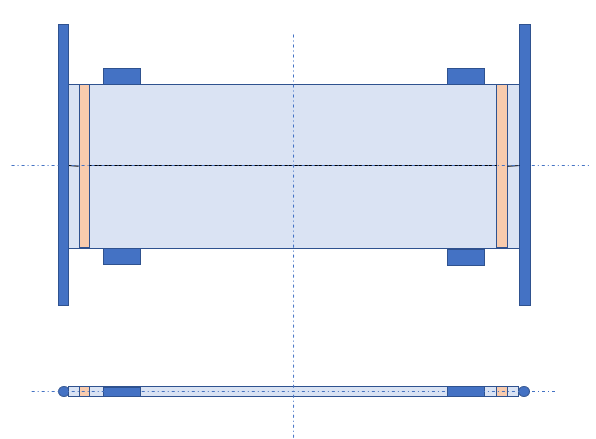
\includegraphics[width=0.30\textwidth]{Bilder/Powerpoint/Gummiband_Klemme}
  \end{center}
  \caption{Gummiband Klemme}
  \label{Gummiband Klemme}
  \vspace{-10pt}
\end{wrapfigure}

Die Gummiband-Klemme hat eine starke Klemmkraft, dies schützt vor dem Aufplatzen der Verpackung. Das Problem dieser Variante ist, dass das Gummiband spröder werden kann und irgendwann reißen kann, also ein hoher Wartungsaufwand. Die Klemmen können auch nicht nach der Entfernung kontrolliert gesammelt werden. Somit könnten sie an unzugänglichen Stellen fallen.

\subsection{Klemmen Wahlvariante}

Jede Klemme hat gewisse Vor- und Nachteile. Deshalb wurden alle Varianten miteinander Verglichen und die am besten geeignete Klemme ausgewählt.

Die folgenden Punkte zeigen warum, die Hebelklemme für unsere Maschine geeignet ist.

\begin{itemize}
\item Durch den Hebel lässt sich die Klemme leicht öffnen, indem sich das Förderband bewegt, die Lasche durch eine Stange eingefädelt wird und diese durch die Bewegung in Richtung Walze geöffnet werden soll.
\item Weil die beiden Metallplatten aufeinander pressen hält die Verpackung durch den besonderen Verschluss Luftdicht zusammen (siehe Abbildung: \ref{Hebel Klemme}). 

\end{itemize} 

\subsection{Futterschüsseln}

Bei den Futterschüssel mussten bestimmte Faktoren erfüllt werden bzw. auf wählerische Katzen abgestimmt werden. Deshalb konnte nicht die einfachste Variante genommen werden die am  den wenigsten Aufwand bedeutet hätte. 

\subsubsection{Drehfutterplatte}

\begin{wrapfigure}{r}{0.5\textwidth}
\vspace{-40pt}
  \begin{center}
    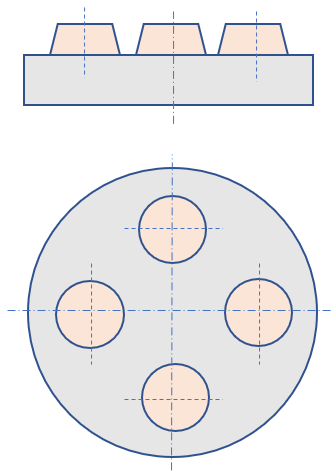
\includegraphics[width=0.25\textwidth]{Bilder/Powerpoint/Drehplatte}
  \end{center}
  \caption{Drehplatte}
  \label{Drehplatte}
  \vspace{-20pt}
\end{wrapfigure}

Die Drehplatte besteht aus fünf Schüsseln. Man kann pro Schüssel die Katze 2-mal pro Tag füttern z.B morgens und abends. Dadurch hat die Katze jeden Tag eine neue Schüssel und falls sie nicht frisst muss sie nicht Hunger leiden(Da Katzen wählerisch sein können, wenn Futter länger herum steht). Auf einer Welle wird eine Platte befestigt. 
Darin werden fünf Löcher geschnitten und die Schüssel hinein gelegt. Die Drehplatte wird mit einem Schneckengewinde in die gewünschten Position gebracht. Siehe Abbildung: \ref{Drehplatte} 

\subsubsection{Futterplatte Zylinder}

\begin{wrapfigure}{r}{0.5\textwidth}
\vspace{-20pt}
  \begin{center}
    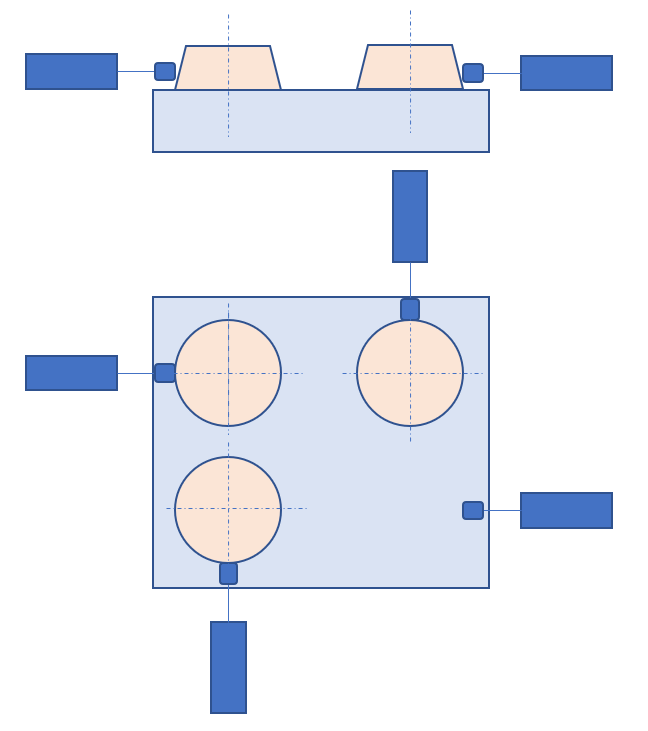
\includegraphics[width=0.32\textwidth]{Bilder/Powerpoint/Platte_Zylinder}
  \end{center}
  \caption{Platte Zylinder}
  \label{Platte Zylinder}
\vspace{-60pt}
\end{wrapfigure}

Die Futterplatte mit Zylinder ist die umständlichste Variante. Es ist eine viereckige Platte auf der Schienen für das Schieben der Futterschüsseln platziert sind. Diese werden von Magnetzylindern angeschoben. Der Nachteil hierbei ist, dass viele Bauteile benötigt werden und alle Zylinder müssen aufeinander abgestimmt arbeiten um die Futterschüssel zur richtigen Position zu führen. Siehe Abbildung: \ref{Platte Zylinder} 

\newpage


\subsubsection{Platte mit einer Schüssel}

\begin{wrapfigure}{r}{0.5\textwidth}
\vspace{-20pt}
  \begin{center}
    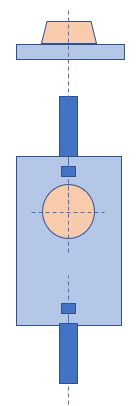
\includegraphics[width=0.10\textwidth]{Bilder/Powerpoint/Einschuessel_platte}
  \end{center}
  \caption{Einschüsselplatte}
  \label{Schüssel Eins}
  \vspace{-10pt}
\end{wrapfigure}

Die Platte mit nur einer Schüssel ist leicht zu realisieren, da sie nur wenige Bauteile benötigt. Das wäre zum Einen die Platte inklusive Futterschüssel und Schiene und zum Anderen auch die zwei Magnetzylinder, die die Futterschüssel in die Anfangs und Endposition bringen. Ein großer Nachteil weswegen diese Methode nicht in Frage kommt ist folgendes: Wenn die Katze nach dem Füttern nicht frisst dann bleibt der Inhalt in der Schale und trocknet ein oder es kommt Ungeziefer hinein. Das hat zu Folge, dass die Schüssel jeden Tag befüllt wird und eventuell übergeht. Siehe Abbildung: \ref{Schüssel Eins} 

\subsection{Futterschüssel Wahlvariante}

Die verschiedenen Futterschüssel-Varianten haben große Vor- bzw. Nachteile bezüglich Platzbedarf und Futterschlüsselanzahl. Diese wurden gründlich durchdacht. Die Wahlvariante ist die Drehplatte die Gründe dafür werden in den Punkten erörtert: 

\begin{itemize}
\item Ein großes Thema war die Anzahl der Futterschüsseln, hierbei war es wichtig, dass die Katze jeden Tag eine reine Schüssel zur Verfügung hat.
\item Die Schüsseln sollten leicht zu entfernen sein und die Oberfläche der Platte ebenfalls leicht zu reinigen sein.
\item Da die Platte auf einer Welle sitzt lässt sie sich durch den Motor in die Befüll- bzw. Fütterungsposition bringen.
\end{itemize} 

\subsection{Futtermagazine}

Diese Futtermagazine waren für die 1.Variante relevant, bei diesen war es wichtig die Packungen so einfach wie möglich in die Schneideposition zu bringen. 

\subsubsection{Futtermagazin Horizontal}

\begin{wrapfigure}{r}{0.5\textwidth}
\vspace{-40pt}
  \begin{center}
    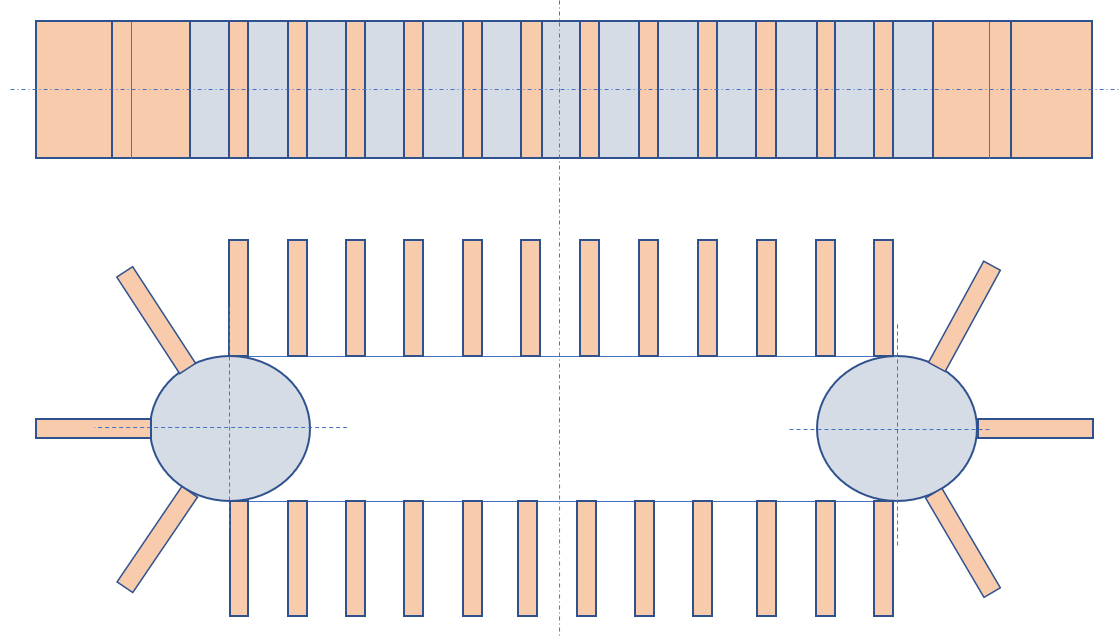
\includegraphics[width=0.30\textwidth]{Bilder/Powerpoint/Futtermagazin_horizontal}
  \end{center}
  \caption{Futtermagazin Horizontal}
  \label{Magazin Horizontal}
  \vspace{-10pt}
\end{wrapfigure} 

Das Futtermagazin Horizontal wäre für die erste Variante optimal. Da man den gewünschten Vorrat an Futterpackungen in die abgetrennten Räume platziert. Somit ist es einfach die gewünschte Position anzufahren und die Packungen mit einen Greifer in die Schneideposition zu bringen. Der Aufbau ist wie ein Förderband, nämlich zwei Räder, ein Band mit oben platzierten Trennwänden und ein Motor der dieses Futtermagazin in Bewegung bringt. Zu beachten wäre wie die Futterpackungen ins Magazin eingelegt werden, nämlich mit der dünneren Fläche mit der Einkerbung die der Hersteller angegeben hat in Richtung Futterplatte. Siehe Abbildung: \ref{Magazin Horizontal}

\subsubsection{Futtermagazin Vertikal}

\begin{wrapfigure}{r}{0.5\textwidth}
\vspace{-40pt}
  \begin{center}
    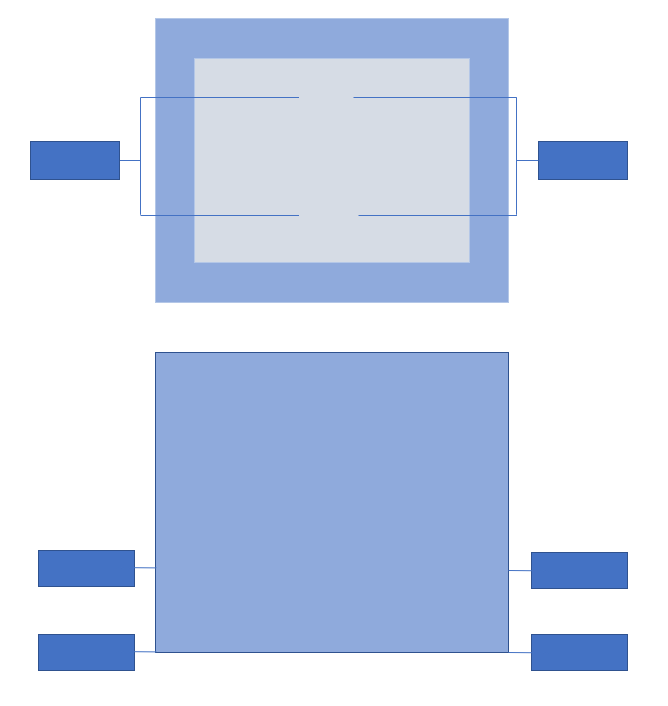
\includegraphics[width=0.36\textwidth]{Bilder/Powerpoint/Futtermagazin_vertikal}
  \end{center}
  \caption{Futtermagazin Vertikal}
  \label{Magazin Vertikal}
  \vspace{-10pt}
\end{wrapfigure}

Das Futtermagazin Vertikal ist ein rechteckiges Gehäuse an denen 4 Magnetzylinder platziert werden(Die mit Kreise versehrten Blöcke). In diese Box kommen die 10 Futterpackungen. Der Ablauf funktioniert in folgenden Reihenfolge. Zuerst öffnet sich der erste linke Magnetzylinder(roter Kreis) danach der gegenüberliegende zweite Magnetzylinder(gelber Kreis). Daraufhin gelangt die erste Futterpackung auf die unteren Zylinder(beiden grünen Kreise). Nach diesem Schritt schließen sich die beiden Magnetzylinder wieder, damit die anderen Packungen nach dem Öffnen der unteren Magnetzylinder nicht durch die Maschine fallen. Daraufhin wenn der Fütterungsbefehl kommt öffnen sich die unteren Zylinder (beiden grünen Kreise)und die Packung gleitet über ein Blech zur Schnittfläche. Der große Nachteil dieser Methode ist, dass immer wieder Fehler auftreten können. Die Futterpackung kann falsch an der Schneidfläche ankommen bzw. sich an einem bestimmten Ort verkeilen. Siehe Abbildung: \ref{Magazin Vertikal}


\section{Konstruktion der Wahlvariante und Details}

\subsection{Drehplatte}

\begin{wrapfigure}{r}{0.5\textwidth}
\vspace{-20pt}
  \begin{center}
    \includegraphics[width=0.30\textwidth]{Bilder/Inventor/Drehplatte}
  \end{center}
  \caption{Drehplatte Inventor}
  \label{Drehplatte_Inventor}
  \vspace{-10pt}
\end{wrapfigure}

Die Drehplatte besteht aus Aluminium und ist 10mm dick. Es werden 5 Löcher für die Schüsseln ausgeschnitten und in der Mitte ist ein Loch, in der eine Stahlwelle durch führt. Die Stahlwelle wurde deshalb ausgewählt, da sie erstens stabiler ist und somit kleiner bzw. mit kleinerem Durchmesser gewählt werden kann. Zweitens ist der Vierkant der Motorwelle 4x4x20, dies ist für Aluminium sehr schmal da große Kräfte auftreten können und der Stift abreißen könnte. Die Drehplatte wird auf der Welle mit einem Flansch befestigt damit das vertuschen nach oben, unten und zur Seite verhindert wird. Siehe Abbildung: \ref{Drehplatte_Inventor} \\

\begin{wrapfigure}{r}{0.5\textwidth}
\vspace{-20pt}
  \begin{center}
    \includegraphics[width=0.26\textwidth]{Bilder/Inventor/Schuessel}
  \end{center}
  \caption{Futterschüssel Inventor}
  \label{Futterschuessel_Inventor}
  \vspace{-40pt}
\end{wrapfigure}

Die Futterschüssel hat deshalb einen Rand damit sie in ein Loch gelegt werden kann ohne dass sie durchfliegt, dennoch lässt sie sich leicht raus nehmen und reinigen. Durch eine rutschfeste Unterlage verrutsch die Schüssel nicht, auch wenn die Katze daraus frisst und sie mit Kraft die Schüssel zu verschieben versucht. \\ Siehe Abbildung: \ref{Futterschuessel_Inventor}. \\


\begin{wrapfigure}{r}{0.5\textwidth}
\vspace{-20pt}
  \begin{center}
    \includegraphics[width=0.35\textwidth]{Bilder/Inventor/Drehplatte_Welle}
  \end{center}
  \caption{Drehplattenwelle Inventor}
  \label{Drehplatte_Welle_Inventor}
  \vspace{-40pt}
\end{wrapfigure}

Die Welle wird aus Stahl konstruiert damit der Vierkant (grüner Kreis) durch das Drehmoment des Motors nicht abreißt. Die Welle wird senkrecht auf die Grundplatte montiert. Ein Lager wird in den Boden gefräst und die Welle auf dem Lager platziert. Auf der oberen Seite der Welle wird der Motor angesteckt. \\ Siehe Abbildung: \ref{Drehplatte_Welle_Inventor} 

\subsection{Förderband, Kettenglied, Kettenrad und Welle}

\begin{figure}[H]
\begin{center}
\includegraphics[width=10cm]{Bilder/Inventor/Kette}
\caption{Kette Inventor}
\label{Kette_Inventor} 
\end{center}
\end{figure}


Das Förderband Abbildung: \ref{Kette_Inventor} weist die z-Achse senkrecht nach oben die x-Achse nach links und die y-Achse nach rechts. Die Konstruktion wird in den folgenden Punkten beschrieben:

\begin{itemize}
\item[1] Als erstes wurde die Sicht in Inventor nach Vorne gedreht um die Grundlage des Förderbandes zu zeichnen.
\item[2] Zweitens wurde die Ebene YZ sichtbar gemacht und eine Ebene mit Versatz erstellt, die 234,95mm entfernt ist. In diesen beiden Ebenen kommen später die Kettenräder.
\item[3] Drittens wird auf der XY Ebene einen Kreis mit einen Durchmesser von 53,068mm gezeichnet. Der zweite Kreis in der gleiche Größe wird auf der erstellten Ebene platziert(234,95mm von der ersten Ebene entfernt). 
\item[4] Viertens werden die beiden Kreise an den obersten und untersten Punkten verbunden. Siehe gelber und roter Kreis.
\item[5] Fünftens wird an den beiden untersten Positionen der Kreise ein Punkt platziert. In Inventor existiert eine Methode namens Muster. Diese Funktion wird auf den Punkten platziert und die Richtung des Pfeiles nach rechts gedreht. Nun wird die Anzahl der Kettenglieder angegeben in unseren Fall 50. Die werden gleichmäßig über die Skizze verteilt.
\item[6] Sechstens wird eine neue Datei erstellt und das Kettenrad aus dem Inhaltscenter platziert. Siehe Abbildung \ref{Kettenrad_Inventor}.
\item[7] Siebtens wird das Kettenglied konstruiert und alle 3 Komponenten in ein gemeinsames Projekt eingefügt. Siehe Abbildung: \ref{Kettenglied_Inventor}.
\item[8] Achtens wird das Kettenglied am untersten Punkt des rechten Kreises abhängig gemacht.
\item[9] Neuntens kann durch die Funktion "Muster" das Kettenglied gleichmäßig auf der Zeichnung verteilt werden und dadurch entsteht die fertige Kette.
\item[10] Zehntens werden die Kettenräder auf den zuvor erstellten Ebenen abhängige gemacht. Danach ist die Kette fertig erstellt.\\
\end{itemize}

Das Kettenglied ist im Handel erhältlich. Die Anfertigung hat auf der Seite einen rechten Winkel auf denen Aluminiumplatten platziert sind. Auf diese Aluminiumplatten wird der Futterbeutel platziert. Siehe Abbildung: \ref{Kettenglied_Inventor}.\\

Das Kettenrad wurde aus dem Inhaltscenter platziert. Danach wurde eine Skizze angelegt und das Loch in der die Welle durch führen soll gezeichnet. Die Rundung für die Passfeder wurde darauf hin auch konstruiert damit das Kettenrad nicht auf der Welle durchrutscht und das Drehmoment übertragen kann. Siehe Abbildung: \ref{Kettenrad_Inventor}.

\begin{figure}[H]
   \begin{minipage}[hbt]{.4\linewidth} % [b] => Ausrichtung an \caption
      \includegraphics[width=\linewidth]{Bilder/Inventor/Kettenglied}
      \caption{Kettenglied Inventor}
      \label{Kettenglied_Inventor} 
   \end{minipage}
   \hspace{.2\linewidth}% Abstand zwischen Bilder
   \begin{minipage}[hbt]{.35\linewidth} % [b] => Ausrichtung an \caption
      \includegraphics[width=\linewidth]{Bilder/Inventor/Kettenrad}
      \caption{Kettenrad Inventor}
      \label{Kettenrad_Inventor}
   \end{minipage}
\end{figure}


\begin{wrapfigure}{r}{0.5\textwidth}
\vspace{-20pt}
  \begin{center}
    \includegraphics[width=0.35\textwidth]{Bilder/Inventor/Antriebs_Welle_Foerderband}
  \end{center}
  \caption{Förderbandwelle Inventor}
  \label{Antriebs_Welle_Foerderband_Inventor}
  \vspace{-30pt}
\end{wrapfigure}

Die Antriebswelle wurde aus Stahl konstruiert um den Vierkant(grüner Kreis) nicht während des Benutzens der Förderbandwelle durch den Motor abzureißen. Die Welle wird an den beiden Stützen gelagert. Siehe Abbildung: \ref{Antriebs_Welle_Foerderband_Inventor}.\vspace{60pt}


\subsection{Walze}

\begin{wrapfigure}{r}{0.5\textwidth}
\vspace{-20pt}
  \begin{center}
    \includegraphics[width=0.26\textwidth]{Bilder/Inventor/Rolle}
  \end{center}
  \caption{Walze Inventor}
  \label{Walze_Inventor}
  \vspace{-20pt}
\end{wrapfigure}

Die beiden Walzen sind aus Kunststoff und innen hohl. Diese sind auch nicht auf der Welle befestigt sondern können sich frei drehen. Es ist nur auf jeder Seite ein Sicherungsring damit die beiden Walzen ihre Postion axial nicht verlassen. Siehe Abbildung: \ref{Walze_Inventor}. \\
\newpage

\begin{wrapfigure}{r}{0.5\textwidth}
\vspace{-20pt}
  \begin{center}
    \includegraphics[width=0.26\textwidth]{Bilder/Inventor/Feder}
  \end{center}
  \caption{Feder Inventor}
  \label{Feder_Inventor}
\end{wrapfigure}

Die Feder drückt die beiden Walzen aneinander um die Futterpackung die durchgezogen wird auszuquetschen. Ohne die Feder und Walze könnte zu viele Reste in der Packung bleiben und so das ganze Futter verschwendet werden. Die Feder wurde von uns konstruiert und auf eine eigene Konstruktion gehängt unabhängig von der Welle, damit die Feder nicht mitgedreht wird, sondern fix an einem Platz positioniert ist an den sie ihre Arbeit verrichtet. \\Siehe Abbildung: \ref{Feder_Inventor}.\\

\begin{wrapfigure}{r}{0.5\textwidth}
\vspace{-20pt}
  \begin{center}
    \includegraphics[width=0.26\textwidth]{Bilder/Inventor/Walzen_Welle}
  \end{center}
  \caption{Welle für die Walze Inventor}
  \label{Walzen_Welle_Inventor}
\end{wrapfigure}

Auf die Aluminiumwalze wurde die Welle die nicht am Grundgerüst ist angesteckt und mit Sicherungsringe gesichert damit die in gleicher position wie die Welle am Grundgerüst ist bleibt. Siehe Abbildung: \ref{Walzen_Welle_Inventor}.\\ 
\subsection{Hebelklemme}

\begin{wrapfigure}{r}{0.5\textwidth}
\vspace{-20pt}
  \begin{center}
    \includegraphics[width=0.3\textwidth]{Bilder/Inventor/Hebel_Klemme}
  \end{center}
  \caption{Hebel Klemme}
  \label{Hebel_Klemme_Inventor}
\end{wrapfigure}

Die Hebelklemme dient zum Optimalen klemmen der Verpackung.
Es ähnelt einen Marmeladenglasverschluss von früher. Die Packung wird zwischen den zwei Platte eingelegt, danach wird der Schließmechanismus auf der oberen Platten eingehakt, siehe roter Kreis. Daraufhin wird die Unterseite des Schließmechanismus nach unten gedrückt, siehe blauer Kreis.
Der Hebel wird soweit nach unten gedrückt bis er beim Stopper auftrifft, siehe gelber Kreis. Der Stopper hat die Aufgabe, dass der Hebel nicht zu weit geschlossen werden kann. Das hat zufolge das die Klemme leichter aufspringt. Siehe Abbildung: \ref{Hebel_Klemme_Inventor}.



\subsection{Gesamtansicht der Konstruktion}

Bei diesem Abschnitt werden von der Gesamtkonstruktion einzelne Teile, die Probleme verursachen könnten, heraus genommen gezeigt und beschrieben.

\subsubsection{Ansicht des Pressvorganges und gleich halten der Walze}

Es wird beachtet, das der Spalt der beiden Walze ungefähr in der Mitte der Futterschüssel ist, wenn man von oben auf die Maschine schaut. Wäre das nicht der Fall würde das Futter daneben Fallen und am Boden der Maschine landen. Siehe Abbildung: \ref{Pressvorgang_Inventor}.\\

Die Walze, die nur durch die Federn an die Maschine gedrückt wird, muss zusätzlich am Grundgerüst befestigt werden damit die auf gleicher Höhe, wie die an der Maschine befestigte Walze hängt. Siehe Abbildung: \ref{Walzen_Halterung_Inventor}.

\begin{figure}[H]
   \begin{minipage}[hbt]{.4\linewidth} % [b] => Ausrichtung an \caption
      \includegraphics[width=\linewidth]{Bilder/Inventor/Walzen_Ansicht}
      \caption{Pressvorgang}
      \label{Pressvorgang_Inventor} 
   \end{minipage}
   \hspace{.2\linewidth}% Abstand zwischen Bilder
   \begin{minipage}[hbt]{.4\linewidth} % [b] => Ausrichtung an \caption
      \includegraphics[width=\linewidth]{Bilder/Inventor/Aufhaengungs_Ansicht}
      \caption{Walzen Halterung}
      \label{Walzen_Halterung_Inventor}
   \end{minipage}
\end{figure}

\subsubsection{Öffnen und befestigen der Futterpackung}

Die Futterpackung wird am Förderband mit zwei Aluminiumplatten aufgehängt. Es wird die Rückseite der Futterpackung per Hand zusammengepresst und zwischen die beiden Platten gelegt. Danach werden die Flügelmuttern angezogen. Auf der Oberseite der Futterpackung wird nach dem hoch quetschen des Futters per Hand die Klemme über den vom Benutzer hergestellter Schneidelinie befestigt. Diese Linie wird mit z.B einer Schere durchtrennt. Siehe Abbildung: \ref{Futterpackung_Aufhaengung_Inventor}.\\

Die Klemme wird durch einen 1 cm dicken gebogenen Draht, ähnelt einen Blitzableiter, geöffnet. Indem dieser am Ende einen leichten Haken hat in der der Hebel einhaken kann. Der Draht wir mit zwei Halterungen an der Grundplatte befestigt. Siehe Abbildung: \ref{Oeffnen_Futterpackung_Inventor}.

\begin{figure}[H]
   \begin{minipage}[hbt]{.4\linewidth} % [b] => Ausrichtung an \caption
      \includegraphics[width=\linewidth]{Bilder/Inventor/Fluegelmutter_Ansicht}
      \caption{Futterpackung Aufhängung}
      \label{Futterpackung_Aufhaengung_Inventor} 
   \end{minipage}
   \hspace{.1\linewidth}% Abstand zwischen Bilder
   \begin{minipage}[hbt]{.4\linewidth} % [b] => Ausrichtung an \caption
      \includegraphics[width=\linewidth]{Bilder/Inventor/Futterpackung_Ansicht}
      \caption{Öffnen der Futterklemme}
      \label{Oeffnen_Futterpackung_Inventor}
   \end{minipage}
\end{figure}

\subsubsection{Gesamtkonstruktion}

Hier wird die gesamte Konstruktion gezeigt. Das Förderband wurde aus Darstellungsgründen für zwei Tage konstruiert und kann je nach Bedarf erweitert werden. Das Gehäuse wurde weg gelassen um die innere Konstruktion besser zu sehen und diese nur eine Rechteck mit einer Einbuchtung wäre aus der die Katze zur Futterschüssel gelangt. Siehe Abbildung: \ref{Gesamt_Ansicht_Inventor}.

\begin{figure}[H]
\begin{center}
\includegraphics[width=12cm]{Bilder/Inventor/Gesamt_Ansicht}
\caption{Gesamtansicht der Konstruktion}
\label{Gesamt_Ansicht_Inventor} 
\end{center}
\end{figure}

\section{Berechnung und Dimensionierung}

In diesen Teil meiner Diplomarbeit werden Berechnung von wichtigen Teilen bzw. Problemstellen durchgeführt. Es wird bei jeder Berechnung der Schlimmst möglich Fall angenommen.

\subsection{Berechnung der Hebel-Klemme}
\label{Berechnung_der_Hebel-Klemme}
Gewählte Presskraft F = 10N. Die Maße der Fläche auf den die Kraft drückt = 4mm x 20mm x 100mm. Elastizitätsmodul von Aluminium = 0.6*$10^{5}\frac{N}{mm^{2}}$.
Diese Kraft wurde so hoch dimensioniert weil sich beim Klemmen der Verpackung Fleischstücken dazwischen befinden könnten und somit und somit die Flächen auseinander drücken. Siehe Abbildung: \ref{SkizzeKlemme}.

\begin{figure}[H]
   \begin{minipage}[hbt]{.4\linewidth} % [b] => Ausrichtung an \caption
      \includegraphics[width=\linewidth]{Bilder/Powerpoint/Flaechenkraft}
      \caption{Skizze der Klemme}
      \label{SkizzeKlemme} 
   \end{minipage}
   \hspace{.2\linewidth}% Abstand zwischen Bilder
   \begin{minipage}[hbt]{.3\linewidth} % [b] => Ausrichtung an \caption
      \includegraphics[width=\linewidth]{Bilder/Powerpoint/IBerechnung}
      \caption{I-Skizze}
      \label{I_Skizze}
   \end{minipage}
\end{figure}

Formeln zur Berechnung der Durchbiegung in der Mitte der Klemme: \\

Die Skizze zeigt welche Seite h und welche Seite b in der benutzten Formel ist. Siehe Abbildung: \ref{I_Skizze}.
\begin{align*}
I = \frac{b*h^{3}}{12} = \frac{20*4^{3}}{12} = 106.66mm^{4} 
\end{align*}

\begin{align*}
f=\frac{ F*l^{ 3 } }{ 48*E*I} = \frac{10N*100^{3}mm^{3}}{48*0.6*10^{5}\frac{N}{mm^{2}}*106.66mm^{4}} = 0.0325mm
\end{align*}
\newpage
\subsection{Berechnung der Welle von der Drehplatte}

\begin{wrapfigure}[12]{r}{0.5\textwidth}
\vspace{-55pt}
  \begin{center}
    \includegraphics[width=0.3\textwidth]{Bilder/Powerpoint/Torsionsmoment}
  \end{center}
  \caption{Kritischer Punkt an der Welle}
  \label{Torsionsmoment}
\end{wrapfigure}

Bei dieser Berechnung wird überprüft ob der Vierkant auf der Welle mit den Maßen 4mm x 4mm x 20mm ein Drehmoment von maximal 18Ncm vom Motor standhält. Die Platte auf der Welle hat einen Durchmesser von 400mm und einer Höhe von 10mm. Es wird der S235 Stahl verwendet mit einem $\tau_z=165\frac{N}{mm^{2}}$. Siehe Abbildung: \ref{Torsionsmoment}.\\
\\
\\

Hier wird die zurückgelegte Strecke eines Kreisbogens pro Sekunde berechnet, um ungefähr die Drehgeschwindigkeit der Futterplatte abschätzen zu können.

\begin{align*}
J = \frac{1}{2}*r^{2}*A_{ P }*\rho*h=\frac{1}{2}*\frac{ \pi*400^{4}mm^{4} }{16}*800*10^{-9}\frac{ kg }{ mm^{3} }*10mm= 20106kg mm^{2} = 0.020kg m^{2}
\end{align*}

\begin{align*}
\alpha = \frac{ M }{ J }=\frac{ 0.180Nm }{ 0.0201kgm^{2} } = 8.9 \frac{ rad }{ s^{2} }
\end{align*}

Berechnung der Torsionsspannung:

\begin{align*}
\tau_{ vor } = \frac{ M_{ t } }{W_{ t } } = \frac{ 180 Nmm }{ 10.66 mm^{3} } = 16.87\frac{ N }{mm^{2}}
\end{align*}

Wird eine 2-fache Sicherheit angenommen:

\begin{align*}
\tau_z=\frac{165}{2}=82.5\frac{N}{mm^{2}}
\end{align*}

Zum Schluss wird noch kontrolliert ob $\tau_v$ kleiner als $\tau_z$ ist.
Damit wird überprüft ob der Vierkant die Belastung standhält.

\begin{align*}
\tau_v < \tau_z  ->  16.87 \frac{N}{mm^{2}} < 82.5\frac{N}{mm^{2}}
\end{align*}

Fazit der Vierkant hält die Belastung mit Leichtigkeit stand.

\subsection{Berechnung der Umfangskraft der Förderbandes}

Es soll mit einer Presskraft von 400g die Packung durch die Walze ausgequetscht werden. Der Durchmesser der Walze ist 62.7mm.


\begin{figure}[H]
   \begin{minipage}[hbt]{.4\linewidth} % [b] => Ausrichtung an \caption
      \includegraphics[width=\linewidth]{Bilder/Powerpoint/Foerderband_Skizze}
      \caption{Skizze des Förderbandes}
      \label{SkizzeFoerderband} 
   \end{minipage}
   \hspace{.2\linewidth}% Abstand zwischen Bilder
   \begin{minipage}[hbt]{.4\linewidth} % [b] => Ausrichtung an \caption
      \includegraphics[width=\linewidth]{Bilder/Powerpoint/Reibung}
      \caption{Skizze für Reibung}
      \label{SkizzeReibung}
   \end{minipage}
\end{figure}

Mit dieser Formel wird ungefähr das $\mu$ berechnet. Mit f=10mm und den Radius der Walze = 31.35. Entspricht ein Auto im Sand. Siehe Abbildung: \ref{SkizzeReibung}

\begin{align*}
\mu = \frac{10}{31.35} = 0.315
\end{align*}

Es wird die erforderliche Umfangskraft $F_U$ berechnet. Die Normalkraft $F_N$ ergibt sich aus der Zugkraft beider Federn, welche im Kapitel \ref{Berechnung_Feder} ausgerechnet wurde. Siehe Abbildung: \ref{SkizzeFoerderband}
\begin{align*}
F_Q= F_U=\mu_Q*F_N = \mu*2*F_{F} = 0.3*2*3.11N = 1.866N
\end{align*}

Das erforderliche Moment des Motors wird mit dieser Formel errechnet:

\begin{align*}
M_{erf}=F_U*r=2N*31.35mm=62.7Nmm
\end{align*}
\newpage
\subsection{Berechnung der Federkonstante}
\label{Berechnung_Feder}

Hier findet die Berechnung der Federkonstante statt, sowohl als auch die Dimensionierung der Feder.

\begin{figure}[H]
   \begin{minipage}[hbt]{.4\linewidth} % [b] => Ausrichtung an \caption
      \includegraphics[width=\linewidth]{Bilder/Powerpoint/Feder}
      \caption{Skizze von der Feder}
      \label{SkizzeFeder} 
   \end{minipage}
   \hspace{.1\linewidth}% Abstand zwischen Bilder
   \begin{minipage}[hbt]{.4\linewidth} % [b] => Ausrichtung an \caption
      \includegraphics[width=\linewidth]{Bilder/Powerpoint/Federkonstante}
      \caption{Skizze zur Berechnung der Federkonstante}
      \label{SkizzeFederkonstante}
   \end{minipage}
\end{figure}

Berechnung der Federkonstante bei nicht ausquetschen der Packung $l_0$=50mm mit 0N und $l_1$=62.7mm mit 1.962N. Siehe Abbildung: \ref{SkizzeFederkonstante}.

\begin{align*}
k =\frac{m*g}{l_d} = \frac{0.2*9.81}{12.7} = 0.154\frac{N}{mm}
\end{align*}

Bei dieser Rechnung wir die vorherige Annahme überprüft und mithand des Deckers die Federkonstante nachgerechnet. D ist der Durchmesser der Feder und beträgt 11mm. Das kleine d ist die Dicke des Drahtes und beträgt 1mm. Für die Anzahl der Wicklungen steht n mit 50 Umwicklungen. G ist das Schubmodul mit 80000$\frac{N}{mm^{2}}$. Siehe Abbildung: \ref{SkizzeFeder}

\begin{align*}
k=\frac{G*d^{4}}{8*D^{3}*n}=\frac{80000*1^{4}}{8*11^{3}*50} = 0.150\frac{N}{mm}
\end{align*}

Berechnung der Kraft der Feder bei ausquetschen der Packung samt Aluminium Halterung. Mit $l_0$=50mm und $l_1$=70.7mm.

\begin{align*}
F=k*l_d=0.150*20.7mm = 3.11N
\end{align*}

\section{Simulation}
Es werden verschiedene Simulationen erstellt, um die Richtigkeit der Rechnungen zu überprüfen.

\subsection{Simulation der Klemme}

\begin{wrapfigure}[7]{r}{0.5\textwidth}
\vspace{-60pt}
  \begin{center}
    \includegraphics[width=0.3\textwidth]{Bilder/Simulation/Hebel}
  \end{center}
  \caption{Hebel-Klemme Simulation}
  \label{Hebel-Klemme_Simulation}
\end{wrapfigure}

Anhand der Simulation erkennt man, die Biegung der Fläche bei einer einwirkenden Kraft von 10N. Der simulierte Wert siehe Abbildung: \ref{Hebel-Klemme_Simulation} und der berechnete Wert siehe Kapitel \ref{Berechnung_der_Hebel-Klemme} sind nahezu gleich.\\
\\
\\
\\

\subsection{Simulation der Feder}
Die Simulation zeigt die Federauslenkung, welche die Feder bei einer Kraft von 3,11N auseinander drückt siehe Abbildung: \ref{Federauslenkung_Simulation_Simulation}. Der ausgerechnete Federweg beträgt 20,7mm siehe Kapitel \ref{Berechnung_Feder}. \\

\begin{figure}[H]
\begin{center}
\vspace{-20pt}
\includegraphics[width=0.6\textwidth]{Bilder/Simulation/Federauslenkung_Simulation}
  \caption{Federauslenkungs Simulation}
  \label{Federauslenkung_Simulation_Simulation}
\end{center}
\vspace{-10pt}
\end{figure}

\section{Bedienung und Wartung}

Bei der Entwicklung der Maschine wurde darauf geachtet, diese Benutzerfreundlich als nur möglich zu gestalten. Darum lässt sich das Gehäuse der Maschine bis zur Hälfte Aufklappen um den Benutzer einen leichten Zugang zu verschaffen. Es mussten auch keine speziellen Vorkehrungen getroffen werden um den Benutzer zu schützen da es keine gefährlichen Stellen in der Maschine befinden die Personen schaden bzw. verletzen könnten. Die Befestigung der Futterpackungen ist auch ein leichtes durch den großen Platz der zur Verfügung steht und wenn man sich an folgende Schritte hält: 

\begin{itemize}
\item[1] Einspannen der Hinterseite der Packungen auf die Aluminiumplatten des Förderbandes. 
\item[2] Die Hebelklemme kurz nach der vom Futterhersteller vorgeschriebenen Schneidelinie festklemmen. (Dabei zu beachten, dass der Hebel in Richtung der Walze auf der rechten Seite befindet).
\item[3] Mit einer Schere oder Messer die Schneidelinie durchtrennen und den Abfall entsorgen.
\item[4] Die gewünschte Anzahl an Packungen festhängen, maximal 10 Packungen.
\end{itemize} 

Weiteres zur Wartung. Nachdem der Benutzer aus dem Urlaub zurück ist, sollte man folgenden Teile der Maschine reinigen: 

\begin{itemize}
\item[1] Die Walze, hierbei kann durch das Ausquetschen der Packungen etwas Gelee an den beiden Walzen hängen bleiben. Einfach mit einem nassen Tuch diese abwischen.
\item[2] Die Futterschüsseln, können mit der Hand entnommen werden indem man auf der Unterseite der Platte die Schüssel nach oben drückt und mit der freien Hand die nimmt. Danach die Schüssel waschen und in die Platte zurück legen.
\item[3] Die Oberfläche der Futterplatte kann nach dem entfernen der Schüssel mit einem nassen Tuch gereinigt werden..
\end{itemize}


\section{Selbstkritische Analyse und Ausblick}

Das Hauptproblem von meiner konstruierten Variante war das Dichthalten der Packung mit einer Klemme die sich automatisch, wenn das Förderband in Betrieb ist leicht öffnet. Darum wurde von uns die Hebel-Klemme konstruiert. Die beim Betrieb des Förderbandes mit dem Hebel in eine Vorrichtung einhakt und diese dann die Klemme öffnet. \\
\\
Für Nachfolgeprojekte wäre besonders darauf zu achten das die Maschine von automatische gereinigt wird und womöglich eine Schneidefunktion einbauen die den Benutzer mehr entlasten könnte.\\
\\
Wenn ich in Zukunft noch einmal eine Katzenfuttermaschine bauen würde, würde ich diese nicht aus Packungen, sondern aus den kleinen Metallfutterpackungen mit der Lasche als Deckel. Der Benutzer müsste dann nur die Laschen so weit nach oben biegen damit der Deckel nicht aufgeht und in das Magazin einlegen. Die Packung wird daraufhin in Bewegung gebracht und die Lasche durch einen Haken geleitet. Dann öffnet sich die Packung und die Katze kann daraus fressen. Hat den Vorteil immer eine frische Schüssel zu haben und es können theoretisch so viele Packungen wie der Benutzer will in die Maschine eingelegt werden. \\
 
